%!TEX root = foo-thesis.tex

\chapter{Evaluierung}
\label{chap:eval}

Die Evaluierung der beiden Ansätze erfolgt mittels mehrerer Experimente, die in diesem Kapitel dokumentiert und analysiert werden sollen. Abschließend soll eine Zusammenfassung zum Vergleich der Ansätze gegeben werden. Eine Evaluierung besteht dabei neben visuellen und quantitativen Betrachtungen der \textit{Predictions} aus der Messung der \textit{Performance}. Dies umfasst im Wesentlichen die gesamte Prozessierungszeit - ab dem Abschluss der Straßenextraktion bis zum Schreiben der \textit{Prediction}. Für den \textit{Feature-Extraction}-Ansatz wird ferner der maximale Speicherverbrauch, der zu einem beliebigen Zeitpunkt der Verarbeitung erreicht wird, gemessen. Auf den Trainingsprozess selbst wird jeweils nur kurz eingegangen. \\\\
Für einen sinnvollen Vergleich werden alle Experimente auf demselben Rechner ausgeführt, der Teil des Projekts ist und folgende Spezifikationen besitzt:
\begin{itemize}
    \item \textbf{CPU}: Intel\textregistered Core\textsuperscript{\texttrademark} i7-8700 mit 6 Kernen, 12 Threads, einem Prozessortakt von 3,2 GHz und maximalen Turbotakt von 4,6 GHz
    \item \textbf{RAM}: 16GB DDR4 mit 2667 MHz
    \item \textbf{GPU}: NVIDIA\textregistered GeForce\textregistered GTX 1060 mit 6GB GDDR5 Grafikspeicher
\end{itemize}
Um die \textit{Predictions} von Modellen quantitativ evaluieren zu können, existieren verschiedene Maße. Zwei für Klassifizierungen häufig genutzte \citep{Li.Cheng-2018, Zaboli.etal-2019} sind \textit{Precision} und \textit{Recall}, die sowohl für eine gesamte \textit{Prediction} als auch pro Klasse berechnet werden können. Die Berechnung selbst erfolgt ebenfalls mit \texttt{scikit-learn}. Auf eine einzelne Klasse $\mathfrak{K}$ und \textit{Predictions} von Punktwolken bezogen, drückt der \textit{Precision}-Wert $P$ den Prozentsatz der Punkte aus, die als $\mathfrak{K}$ klassifiziert wurden und tatsächlich $\mathfrak{K}$ sind. Der \text{Recall}-Wert $R$ hingegen gibt den Prozentsatz aller $\mathfrak{K}$-Punkte an, die korrekt als $\mathfrak{K}$ klassifiziert wurden. Je nach Anwendungsfall kann der eine oder der andere Wert bedeutsamer sein und höher gewichtet werden. Bei der Anforderung, möglichst alle Schlaglöcher zu finden, ist der \textit{Recall} der entscheidende Wert; bei der Anforderung, nur tatsächlich vorhandene Schlaglöcher zu detektieren, hingegen die \textit{Precision}. Für die in dieser Arbeit behandelte Schadenserkennung sollen beide gleich stark gewichtet werden. Um beide Werte zu einem einzelnen zusammenzufassen und dabei besonders niedrige Ausschläge in einem der beiden zu ahnden, kommt oft der $F_1$-Score zum Einsatz:
\begin{equation}
    F_1 = \frac{2 * P * R}{P + R}
\end{equation}
Für die kommenden Experimente werden jeweils Tabellen aufgeführt mit diesen drei Metriken. Dabei werden sie nur pro Klasse berechnet, da die Werte bezogen auf die Gesamtklassifzierung - aufgrund der um ein Vielfaches höheren Zahl an gewöhnlichen Straßenpunkten gegenüber dem Rest - wenig Aussagekraft besitzen für die Qualität des Ergebnisses. Der Übersicht halber werden in folgenden Tabellen Abkürzungen für Klassennamen verwendet, die zusammen mit der Farbgebung der Klasse in annotierten Punktwolken in Tabelle \ref{table:classes_abbr} aufgeführt sind. Bei Bildern annotierter Punktwolken wird die Klasse der gewöhnlichen Straßenpunkte allerdings nicht zu sehen sein, damit die für diesen Anwendungsfall bedeutsameren Klassen und Unterschiede zwischen \textit{Predictions} besser zu erkennen sind.

\begin{table}
\centering
\begin{tabular}{r|c|c}
& Abkürzung & Farbe \\
\hline
(unbeschädigte) Straße & \textit{U} & / \\
Schlagloch & \textit{S} & hellblau \\
Flickstelle & \textit{F} & gelb \\
Gully & \textit{G} & rot \\
Ölfleck & \textit{Ö} & orange \\
Fahrbahnmarkierung & \textit{M} & schwarz \\
\end{tabular}
\caption{Abkürzungen und Farbgebungen der einzelnen Klassen.}
\label{table:classes_abbr}
\end{table}

\section{Trainings- und Testdaten}

Bei den für Training und Test der Modelle genutzten Punktwolken handelt es sich um zwei separate Abschnitte eines Asphalt-Straßenzugs. Sie sind in bereits extrahierter Form und gemeinsam in Abbildung \ref{fig:train_test_pcs} dargestellt. Die Straße führt an einigen Wohnhäusern mit vereinzelt parkenden Autos entlang. Sie ist in der Stadt Essen gelegen und wurde mit der Art von \textit{Mobile-Mapping}-Fahrzeug erfasst, wie es in Abbildung \ref{fig:mm_vehicle} zu sehen ist. \\

\begin{figure}
    {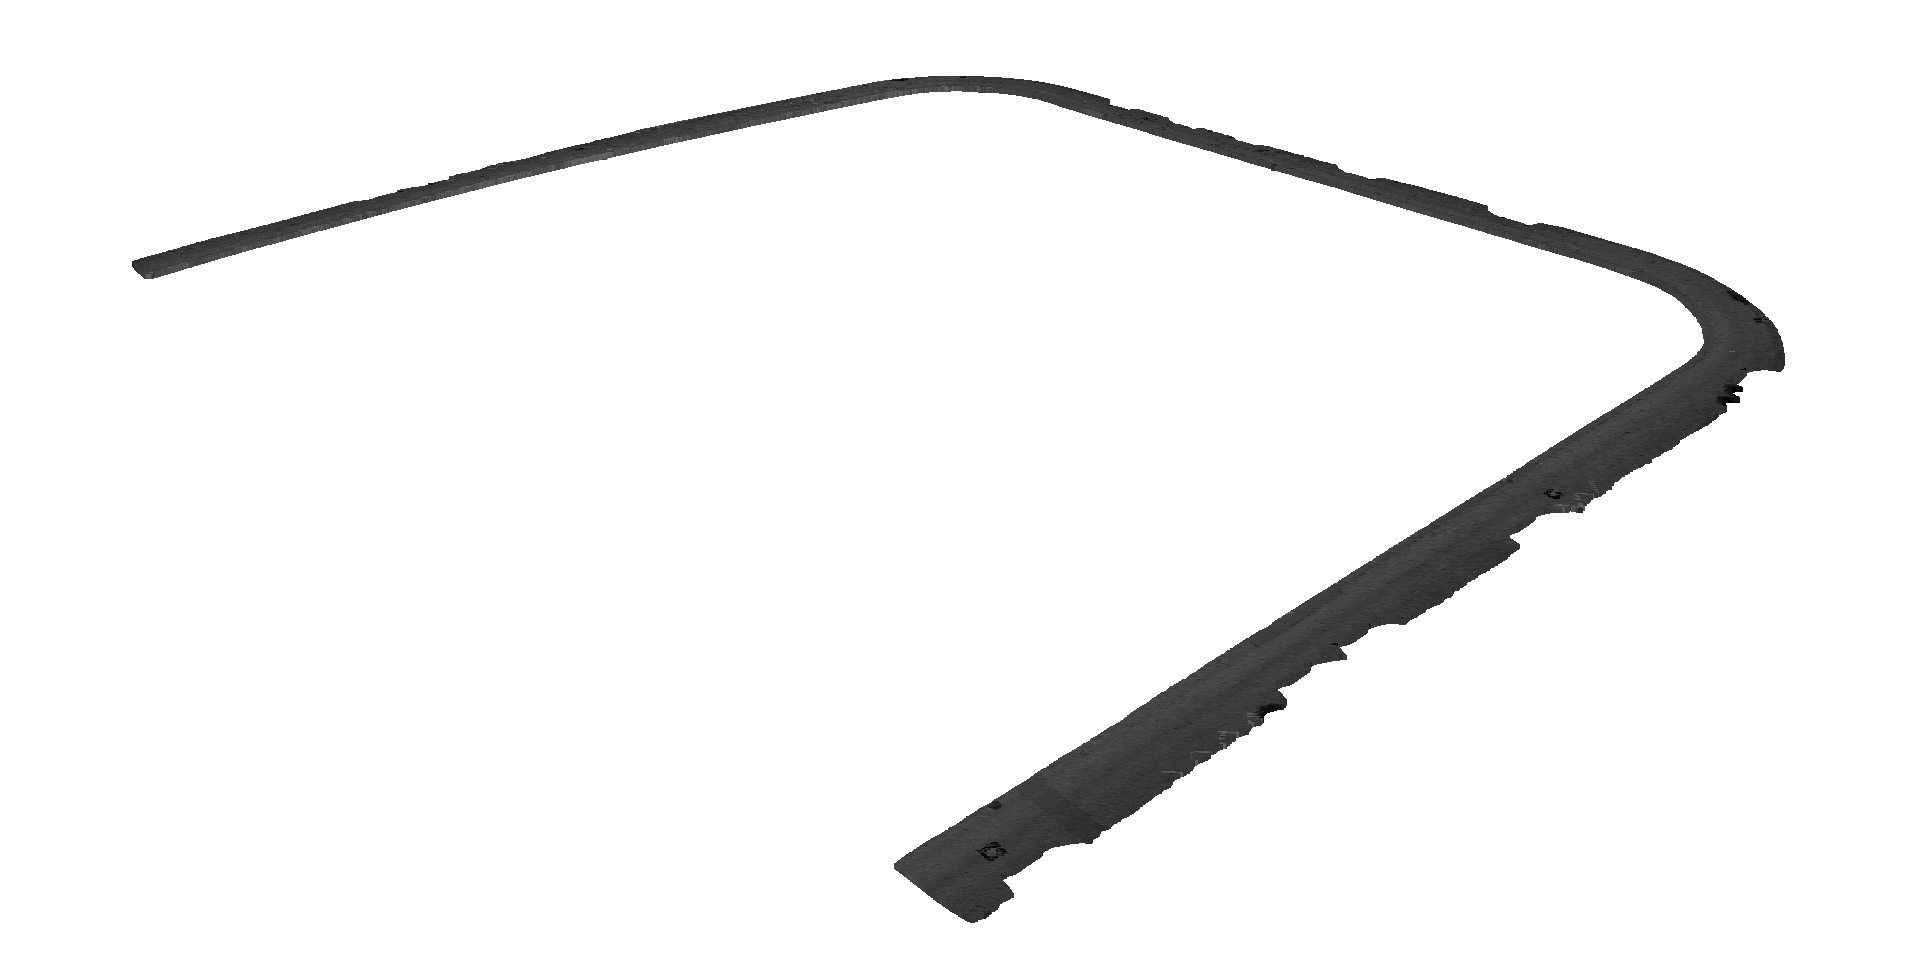
\includegraphics[width=0.8\textwidth]{graphics/full_both}}
    \caption{Der komplette Straßenzug aus Trainings- und Testpunktwolke auf einen Blick.}
    \label{fig:train_test_pcs}
\end{figure}

Einige Kennzahlen zu den Punktwolken in Form der individuellen Klassenhäufigkeiten sind in Tabelle \ref{table:class_frequencies} aufgeführt. Daraus abzuleiten ist, dass die Trainingspunktwolke ungefähr zwischen 1,5 und 2 Mal so groß ist wie die Testpunktwolke, was sich in den jeweiligen Häufigkeiten - abgesehen von den Fahrbahnmarkierungen - annähernd proportional widerspiegelt. Auffällig ist die für den Anwendungsfall typische und bereits angesprochene übergroße Mehrheit der gewöhnlichem Straßenpunkte, die durch deren \textit{Sampling} für das Training reduziert wird. \\

\begin{table}
\centering
\begin{tabular}{c|c|c|c|c|c|c}
 & \textit{U} & \textit{S} & \textit{F} & \textit{G} & \textit{Ö} & \textit{M} \\
\hline
Training & 2571923 & 780 & 35058 & 9521 & 6876 & 1497 \\
Test     & 1467770 & 683 & 20866 & 4670 & 3825 & 4054 \\
\end{tabular}
\caption{Die Klassenhäufigkeiten für die Trainings- sowie Testpunktwolke.}
\label{table:class_frequencies}
\end{table}

Im Gegensatz zu Arbeiten wie \cite{Zhiqiang.etal-2019} sind die hier genutzten Punktwolken dichter und die Straßen in insgesamt besserem Zustand. Die durch Drohnenabtastung entstandenen Punktwolken resultieren dort bei 400$m$ Länge der Straße in etwa 900.000 Punkten und einer Dichte von 40/$m^2$. Die vorgestellte Trainingspunktwolke allein besteht bei etwas über 100$m$ Länge aus mehr als 2,6 Millionen Punkten. Während dort ferner der durchschnittliche Durchmesser von Schlaglöchern bei 50$cm$ liegt, übersteigen hier die größten vorkommenden Schlaglöcher nicht 30$cm$. Diese Diskrepanz spiegelt sich auch in den genutzten Scales wider: Der kleinste Scale beträgt dort 20$cm$ und steigt bis auf 200$cm$ an, während die Spanne hier lediglich von 3$cm$ bis 15$cm$ reicht. Zwar wird die Laufzeit ihres Ansatzes bei \cite{Zhiqiang.etal-2019} nicht genannt, aber mit Blick auf die hohe Dichte und den Laufzeiten ausgewählter größerer Scales in Tabelle \ref{table:bigger_scales} ergibt sich - im Sinne akzeptabler Verarbeitungsdauern für die Webplattform - die Notwendigkeit begrenzt großer Scales.

\section{Preprocessing} 

Im Folgenden sollen kurz die Ergebnisse der Vorverarbeitungsschritte dargestellt werden.

\subsection*{Straßenextraktion}

Die Straßenextraktion wird auf einer Punktwolke mit bereits klassifizierten Bodenpunkten ausgeführt. Diese Bodenerkennung erfolgt mit zuvor durch den Ansatz von \cite{Mattes-2021} ermittelten Parametern. Das Ergebnis dieses gesamten Prozesses für die Trainingspunktwolke ist in Abbildung \ref{fig:street_extraction} visuell dargestellt. Dabei sinkt die Punktmenge von ursprünglich 9,36 Millionen auf 4,84 Millionen nach der Entfernung der Nicht-Bodenpunkte. Infolge der Straßenextraktion verbleiben 4,22 Millionen Punkte. Die Straßenextraktion wird vorsichtig ausgeführt, mit dem Ziel alle Straßenpunkte zu behalten und somit potenziell jeden darauf befindlichen Schaden zu erkennen. Tatsächlich verbleibt in der ausgegebenen Punktwolke jeder Straßenpunkt. Dafür ist auch der dicht vom Laserscanner abgetastete Gehweg erhalten geblieben. Außerdem sind die Autoreifen der ursprünglich dort parkenden Autos weiterhin Teil der Punktwolke, wie im Vordergrund der Abbildung zu erkennen. Diese sind dicht mit der Straße verbunden und mit dem hier vorgestellten Ansatz daher schwerlich davon zu trennen. Deshalb sollte bereits der vorhergehende Schritt der Bodenerkennung sicherstellen, solche Objekte nicht als Boden zu klassifizieren. Die Laufzeit der Straßenextraktion beträgt für diese Punktwolke 78$s$.

\begin{figure}
    {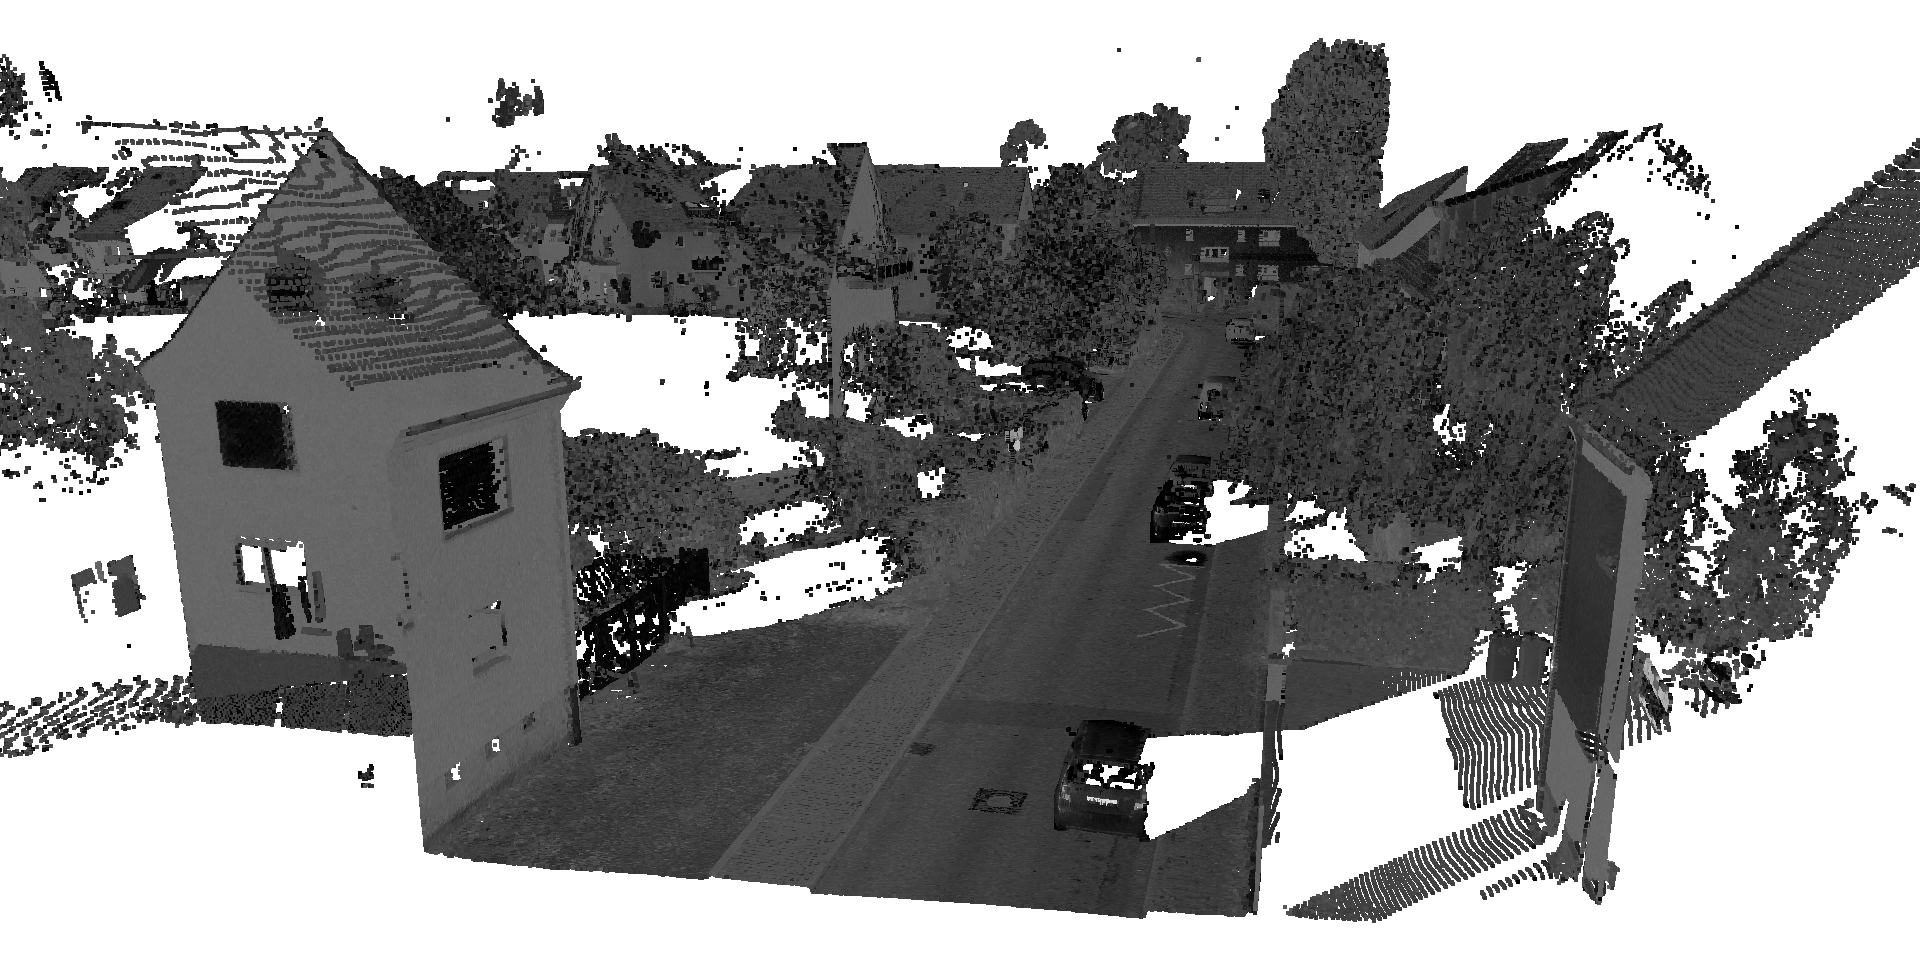
\includegraphics[width=0.96\textwidth]{graphics/eval_street_extr_full}}
    \par\smallskip
    {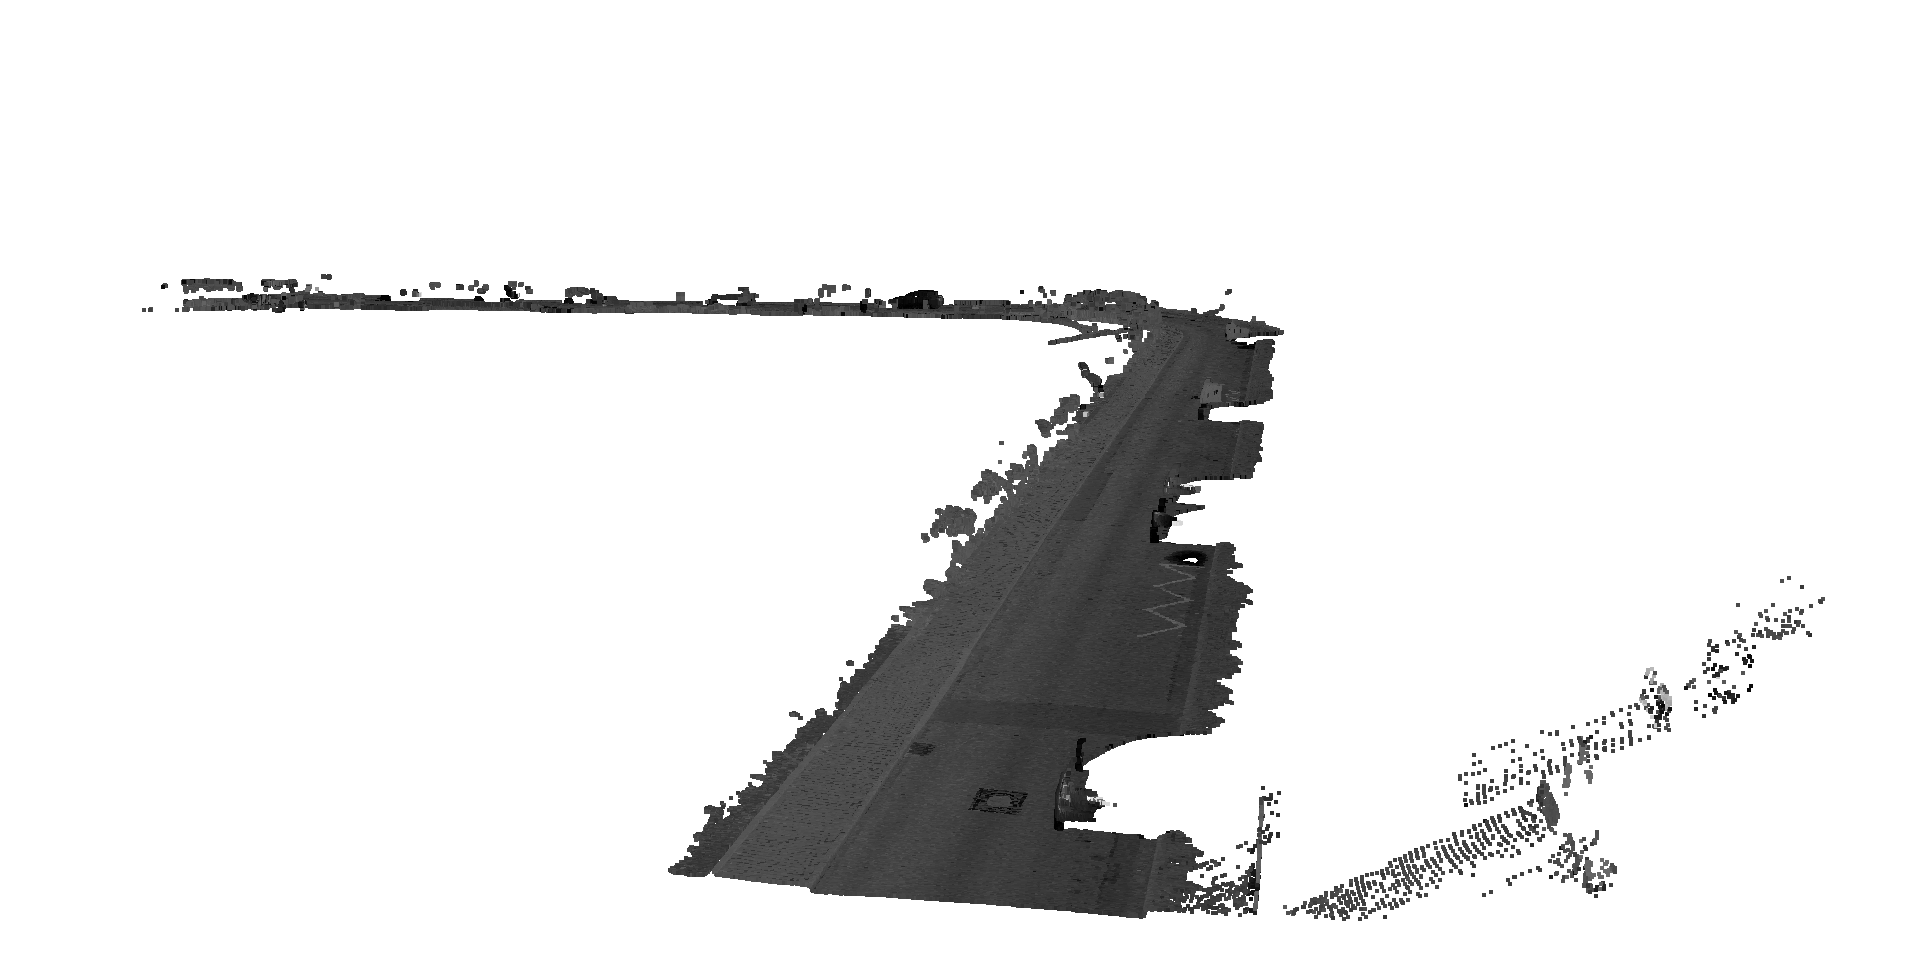
\includegraphics[width=0.96\textwidth]{graphics/eval_street_extr_ground}}
    \par\smallskip
    {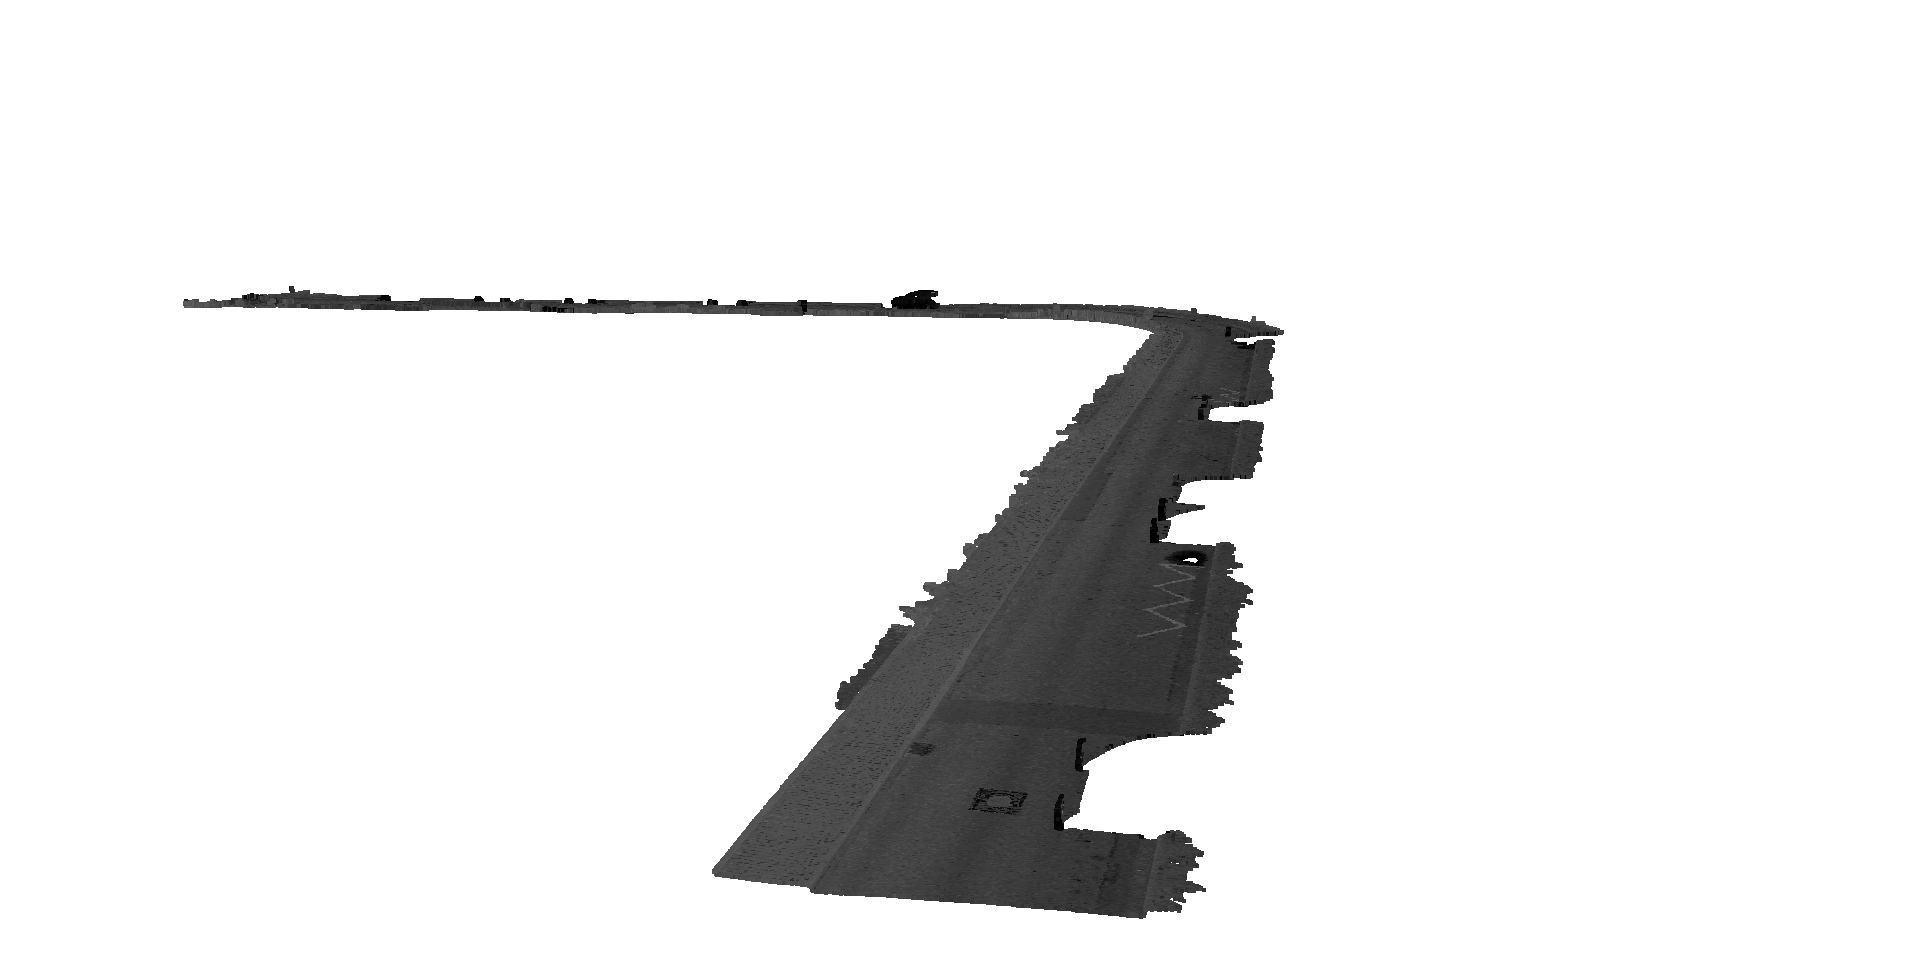
\includegraphics[width=0.96\textwidth]{graphics/eval_street_extr_final}}
    \caption{Die ursprüngliche Punktwolke (oben), nach der Nicht-Bodenentfernung (mittig) und nach der Straßenextraktion (unten).}
    \label{fig:street_extraction}
\end{figure}

\subsection*{Normalisierung der Intensität}

Der erste wesentliche Schritt bei der Featureberechnung ist die Normalisierung der Intensitätswerte, was auch die Entfernung von übermäßig stark abweichenden Werten umfasst. Die minimale und maximale Intensität sowie Kennzahlen vom Entfernen der Außenseiterwerte sind in Tabelle \ref{table:intensity_preproc} zu finden. Insgesamt fällt auf, dass die Testpunktwolke eine etwas größere Streuung der Intensitäten besitzt, zumindest im Bereich zwischen dem ersten und dritten Quartil. Dies ist erkennbar an der marginal größeren \textit{Interquartile Range}. Aus diesem Grund sind auch die Schwellwerte bei der Testpunktwolke näher dran an den tatsächlichen minimalen bzw. maximalen Werten, was zu weniger als Außenseiter betrachteten Punkte führt. Ansonsten sind die Auswirkungen auf die beiden Punktwolken ähnlich, da keine extrem auffälligen Außenseiter vorhanden sind. Am ehesten trifft dies auf die maximale Intensität der Trainingspunktwolke von 30632 zu, wobei der zweitgrößte Wert gleich 29353 ist. Beide Werte werden aber entsprechend angepasst auf 25914. Nach der Normalisierung der teils angepassten Werte beträgt die durchschnittliche Intensität für die Trainingspunktwolke 0,588 bzw. 0,589 für die Testpunktwolke. Die Intensitätswerte sind also vergleichbar und konsistent über die Punktwolken hinweg. \\
Für die konkreten Punktwolken hat der Vorverarbeitungsschritt also keine merklichen Auswirkungen. Im allgemeinen Fall könnte jedoch die Situation auftreten, dass einige wenige Punkte außerordentlich stark reflektieren und einen um mehrere Tausend größeren Intensitätswert besitzen. Solche Werte würden erkannt und entsprechend zurückgesetzt werden. Für den Anwendungsfall der Erkennung von Straßenschäden ist dieser Schritt sinnvoll, da keine Klasse sich (mit so wenigen Punkten) derart stark abheben sollte. Mit einer Laufzeit von knapp 3 Sekunden für die Trainingspunktwolke ist er außerdem - mit Blick auf die Dauer folgender Schritte - schnell ausgeführt.

\begin{table}
\centering
\begin{tabular}{c|c|c|c|c|c|c|c}
 & min & $T_{lo}$ & $\# lo$ entfernt & max & $T_{hi}$ & $\# hi$ entfernt & $IQR$ \\
\hline
Training   & 0 & 1791 & 1049 & 30632 & 25914 & 23 & 2193 \\
Test       & 0 & 928 & 137 & 27939 & 27592 & 4 & 2424 \\
\end{tabular}
\caption{Kennzahlen zur Entfernung von Außenseitern und Normalisierung der Intensitätswerte.}
\label{table:intensity_preproc}
\end{table}

\section{Ansatz Feature Extraction} 

In den folgenden Abschnitten sollen die Ergebnisse der Experimente zum \textit{Feature-Extraction}-Ansatz vorgestellt und analysiert werden. Dabei gilt für alle Experimente, dass sie ohne das \textit{Postprocessing} durchgeführt werden, da dieses im Abschnitt \ref{section:postproc} gesondert evaluiert wird. Ferner wurde in diesen Durchläufen auch nicht das \textit{Uniqueness}-Konzept eingesetzt, außer im gleichnamigen Abschnitt, der spezifisch auf dessen Auswirkungen Bezug nimmt.
Die genutzten \textit{Random Forests} als Modelle sind sehr robust. Auch bei wiederholter Durchführung eines Experiments mit identischen Parametern, trotz randomisierter Abläufe wie dem \textit{Sampling} der Straßenpunkte und der Erstellung der einzelnen Bäume, unterscheiden sich die \textit{Predictions} nur marginal. Die Metriken in Form des \textit{F1-Scores} variieren um weniger als einen Prozentpunkt und auch bei optischer Betrachtung sind nur an einzelnen Punkten Unterschiede erkennbar. Aus diesem Grund sind im Folgenden jeweils nur die Ergebnisse eines einzelnen Durchlaufs dokumentiert.

\subsection{Ergebnis des Basisexperiments}

Die Gesamtdauer des Experiments mit den in Kapitel \ref{chap:feature-calc} erläuterten Scales und Features beträgt knapp 210$s$, was sich aufteilt in 180$s$ für die Featureberechnung im \texttt{PCTool} sowie 30$s$ für die \textit{Prediction} in den Python-Skripten mittels eines trainierten Modells. Das vorher durchgeführte einmalige Training des \textit{Random Forest} dauert 45$s$. Der maximale Speicherverbrauch für die Verarbeitung der Testpunktwolke liegt bei 2,5 GB, die geschriebene Featuresdatei mit den Featurevektoren hat - ohne \textit{Uniqueness} - eine Größe von 1,4 GB. \\
Die Metriken zur \textit{Prediction} des Versuchs finden sich in Tabelle \ref{table:default_metrics}, ein Ausschnitt mit allen betrachteten Klassen ist in Abbildung \ref{fig:cmp_full} gezeigt. Dabei fällt auf, dass die Metriken für die gewöhnlichen Straßenpunkte außerordentlich gut ausfallen. Dies allein trifft jedoch keine Aussage über die Qualität der \textit{Prediction}, da - wie mehrmals erwähnt - diese Klasse um ein Vielfaches häufiger ist die restlichen. Auch die Ölflecken werden gut erkannt, insbesondere mit einer hohen \textit{Precision}. Unter Berücksichtigung der Tatsache, dass es deutlich weniger Trainingsdaten für Fahrbahnmarkierungen gibt als Testdaten, sind deren Ergebnisse akzeptabel. Vor allem werden nahezu keine der in Abbildung \ref{fig:fake_road_marking} angesprochenen Punkte als Fahrbahnmarkierung klassifiziert. Wie Abbildung \ref{fig:road_marking} verdeutlicht, wird die Markierung nahezu durchgängig korrekt klassifiziert bis zum Rand der Punktwolke. Die Punkte am Rand heben sich zwar optisch ebenfalls ab, ihre (absolute) Intensität liegt aber um 17000 und nicht über 20000 wie beim Rest der Fahrbahnmarkierung. Eine solche Intensität besitzen auch viele Punkte, die zur gewöhnlichen Straße gezählt werden. Daher kann davon ausgegangen werden, dass die Trainingsdaten für diese Klasse in zu geringem Maße vorhanden bzw. zu wenig vielfältig sind. \\\\
Die Metriken der Flickstellen liegen im mittleren Bereich. Dies lässt sich mit Blick auf Abbildung \ref{fig:cmp_flickstellen} erklären: Zwar sind in der \textit{Prediction} die grundlegenden Verläufe der Flickstellen erkennbar, die meist Rechtecke bilden. Jedoch ist diese Klassifizierung sehr unbeständig und lückenhaft, teilweise mit Rauschen verbunden. Gleichzeitig ist eine solche unbeständige Stelle in der Abbildung markiert und der Vergleich mit der nach Intensität eingefärbten Punktwolke zeigt, dass dieser Teil der Flickstelle sich tatsächlich kaum in der Intensität abhebt von seiner Umgebung. Auf der anderen Seite zeigt sich bei Stellen, die vermeintlich zu umfangreich als Flickstelle erkannt wurden, dass die Fugendichtmasse mit ihrer geringeren Intensität dort auch wirklich breiter verläuft. Die \textit{Prediction} erfüllt somit die ursprüngliche Idee der genutzten (Intensitäts-)Features, Entscheidungen bezüglich größerer Intensitätsunterschiede zu treffen. Dies führt sogar dazu, dass komplett neue Streifen von Flickstellen als solche klassifiziert werden, obwohl diese nicht so annotiert sind (Abbildung \ref{fig:new_flickstelle}). Auch wenn diese Stelle nicht rechteckig verläuft, sind die Intensitätsunterschiede ersichtlich und es könnte sich somit tatsächlich um eine Flickstelle handeln. Für die ausgelassenen Stellen bedarf es offenbar anderer bzw. weiterer Features oder einer Nachverarbeitung, welche die korrekt klassifizierten Flickstellen zu Rechtecken verbindet. \\\\
Die Gullys werden unabhängig von ihrer Ausprägung grundsätzlich alle erkannt und dabei auch beinahe vollständig. Lediglich die sehr zentralen Punkte des großen Gullys werden als Straße klassifiziert, wie noch leicht in Abbildung \ref{fig:cmp_full} zu erkennen. Der Grund dahinter ist vermutlich ein zu geringer Scale, sodass diese Punkte als Teil einer sehr planaren Umgebung betrachtet werden. Von Vorteil bei den Gullys ist zum einen die große Menge an Trainingsdaten, zum anderen die Tatsache, dass ihre Formen und Größen genormt sind und somit leicht vergleichbar über verschiedene Punktwolken hinweg. Allerdings gibt es einige Stellen unterschiedlicher Charakteristik, die fälschlich als Gully klassifiziert werden. Die beiden häufigsten Arten sind in Abbildung \ref{fig:gully_misclas} vorzufinden: Streifen am Rande der Punktwolke werden als Gullys betrachtet ebenso wie kleine runde Stellen. Gemeinsam ist ihnen, dass sie leichte Erhebungen darstellen, wie sie auch bei Gullys vorkommen. Außerdem zählen insbesondere zu den kleineren, eckigen Gullys deutlich tiefer gelegene Punkte, wie ebenfalls in der Abbildung zu erkennen. Sie entstehen durch Abtastung des Schachts unter dem Kanaldeckel, der relativ breite Öffnungen bietet. Wegen der Struktur dieser Punktmenge besitzen die Punkte verhältnismäßig hohe Werte für \textit{Scattering} und \textit{Curvature}, was ursächlich für die Fehlklassifzierungen sein könnte. Unabhängig von der Ursache könnte es sinnvoll sein, weitere Klassen wie ``Erhebung'' einzuführen. \\\\
Von den fünf Schlaglöchern der Testpunktwolke werden grundsätzlich drei erkannt mit jeweils mehreren Punkten. Dazu zählen die beiden aus Abbildung \ref{fig:cmp_full} sowie das Schlagloch inmitten der Flickstellen aus Abbildung \ref{fig:new_flickstelle}. Bei der Klassifikation von Schlaglochpunkten ist sich das Modell sicher, wie die sehr hohe \textit{Precision} ausdrückt, wohingegen der \textit{Recall} deutlich niedriger ist. Die drei erkannten Schlaglöcher sind mit zu geringem Radius klassifiziert, was erneut für noch zu kleine Scales spricht. Die beiden nicht erkannten Schlaglöcher sind als Gully (mit sehr wenigen Punkten) bzw. Flickstelle klassifiziert, wie Abbildung \ref{fig:cmp_flickstellen} unten zeigt. Ersteres ist kleiner als die anderen Schlaglöcher und könnte aus ähnlichen Gründen wie die Erhebung als Gully erkannt worden sein. Für das zweite Schlagloch gilt, dass es eine deutlich länglichere Form als die anderen aufweist und keine analogen Stellen in der Trainingspunktwolke existieren. In diesem Sinne erscheint die getroffene Klassifikation als Flickstelle wegen der auffälligen Intensität und charakteristischen länglichen Form durchaus plausibel.

\begin{table}
\centering
\begin{tabular}{c|c|c|c|c|c|c}
 & \textit{U} & \textit{S} & \textit{F} & \textit{G} & \textit{Ö} & \textit{M} \\
\hline
Precision & 0,989 & 0,936 & 0,468 & 0,755 & 0,952 & 0,942 \\
Recall    & 0,994 & 0,151 & 0,364 & 0,868 & 0,712 & 0,652 \\
F1        & 0,991 & 0,260 & 0,409 & 0,807 & 0,814 & 0,771 \\
\end{tabular}
\caption{Die Metriken der einzelnen Klassen für das Experiment mit standardmäßigen Scales und Features.}
\label{table:default_metrics}
\end{table}

\begin{figure}
    {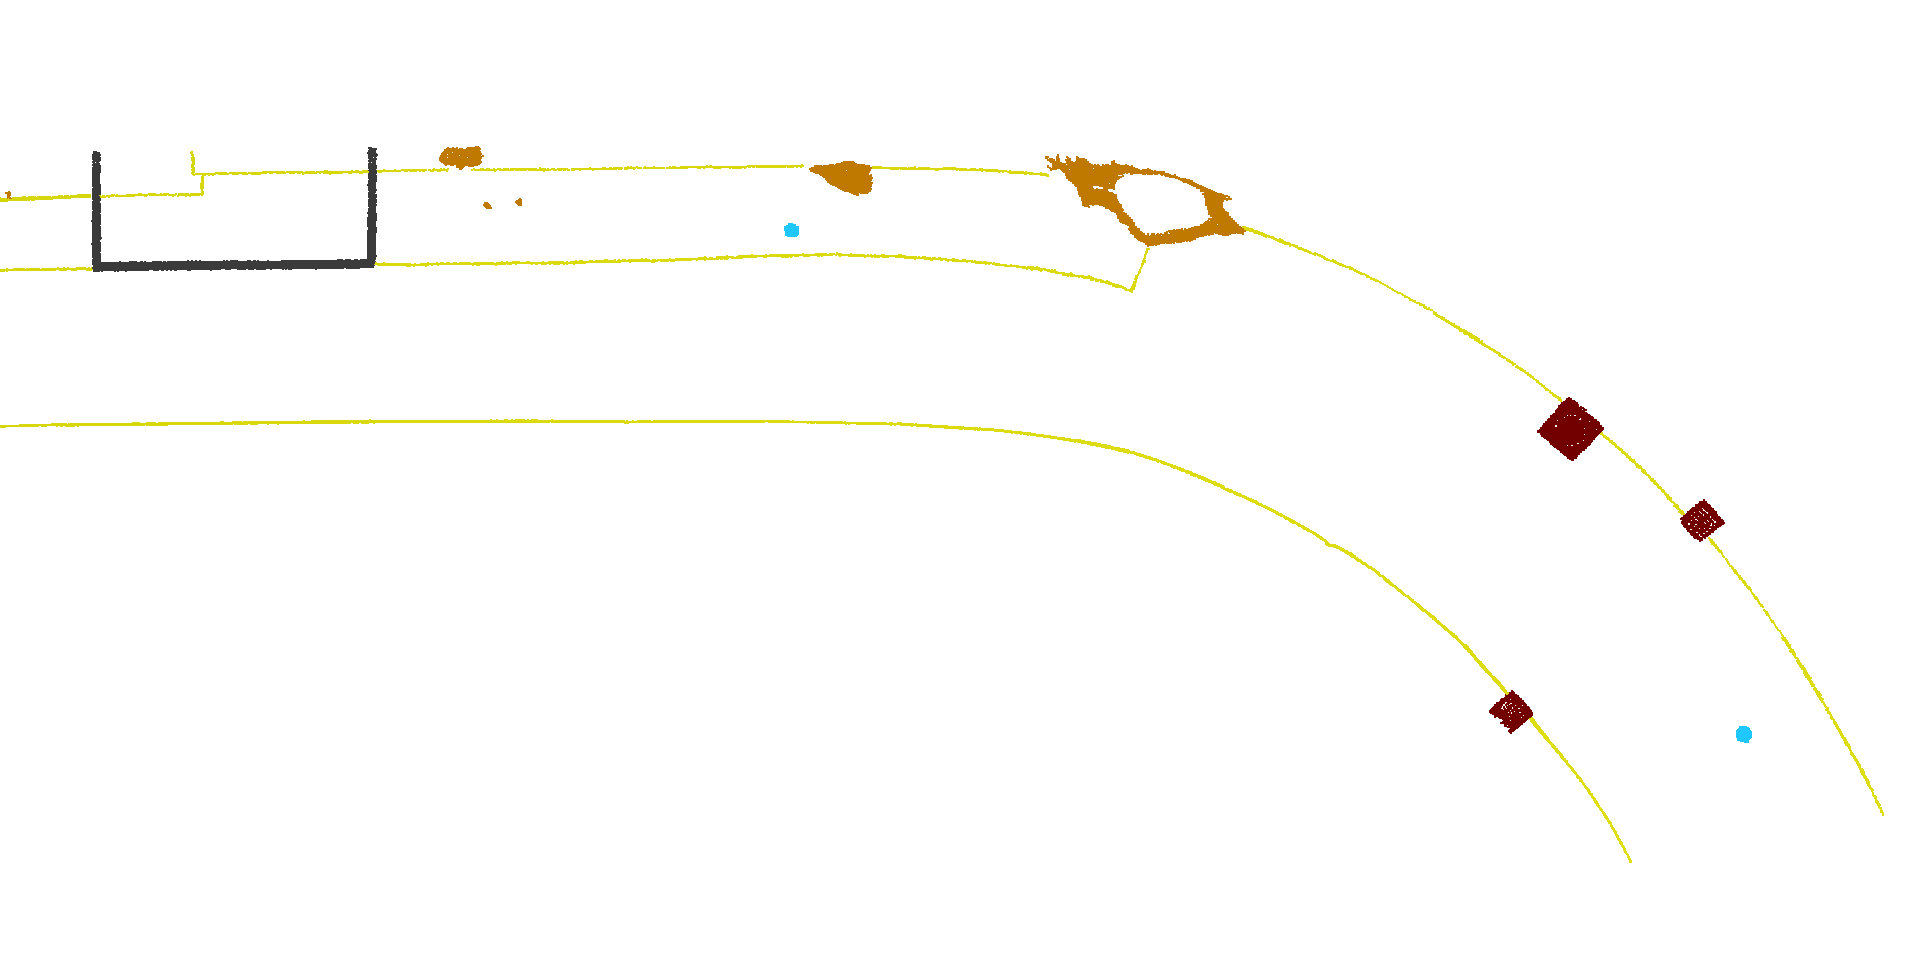
\includegraphics[width=0.96\textwidth]{graphics/eval_right_ground_truth}}
    \par\smallskip
    {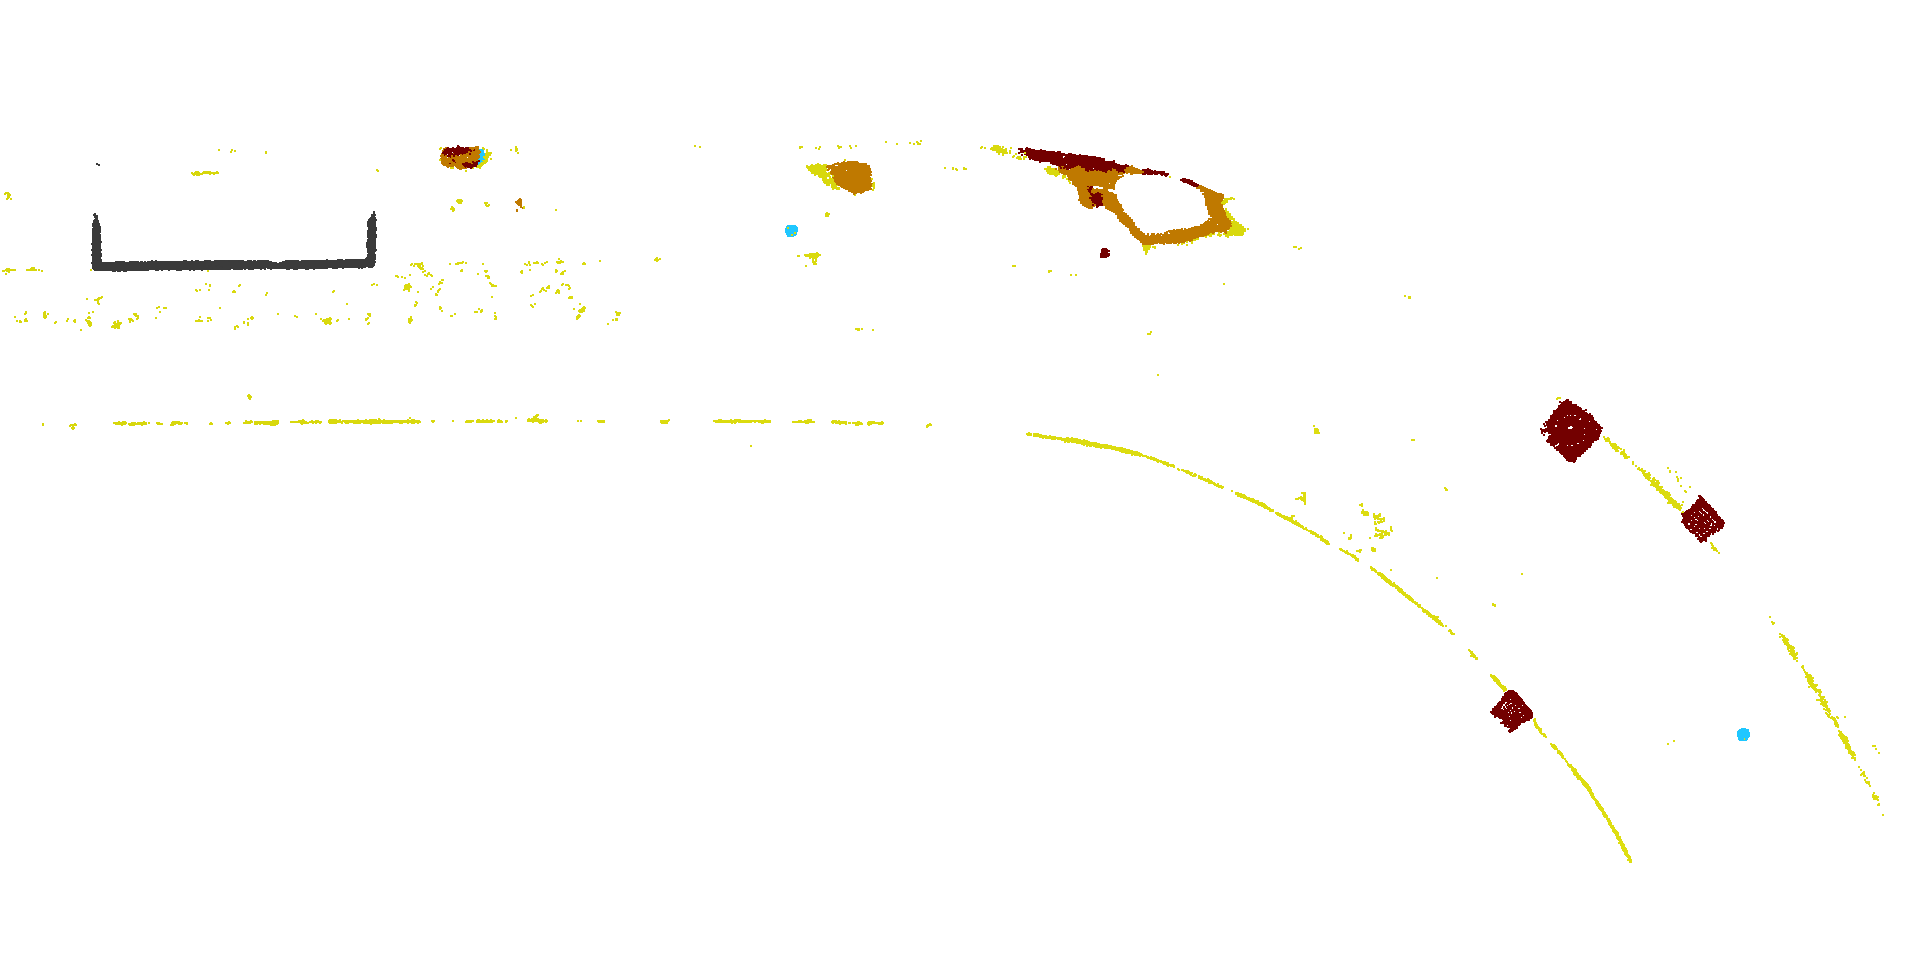
\includegraphics[width=0.96\textwidth]{graphics/eval_right_prediction}}
    \caption{Die tatsächlichen Klassen (oben) und die Prediction (unten).}
    \label{fig:cmp_full}
\end{figure}

\begin{figure}
    {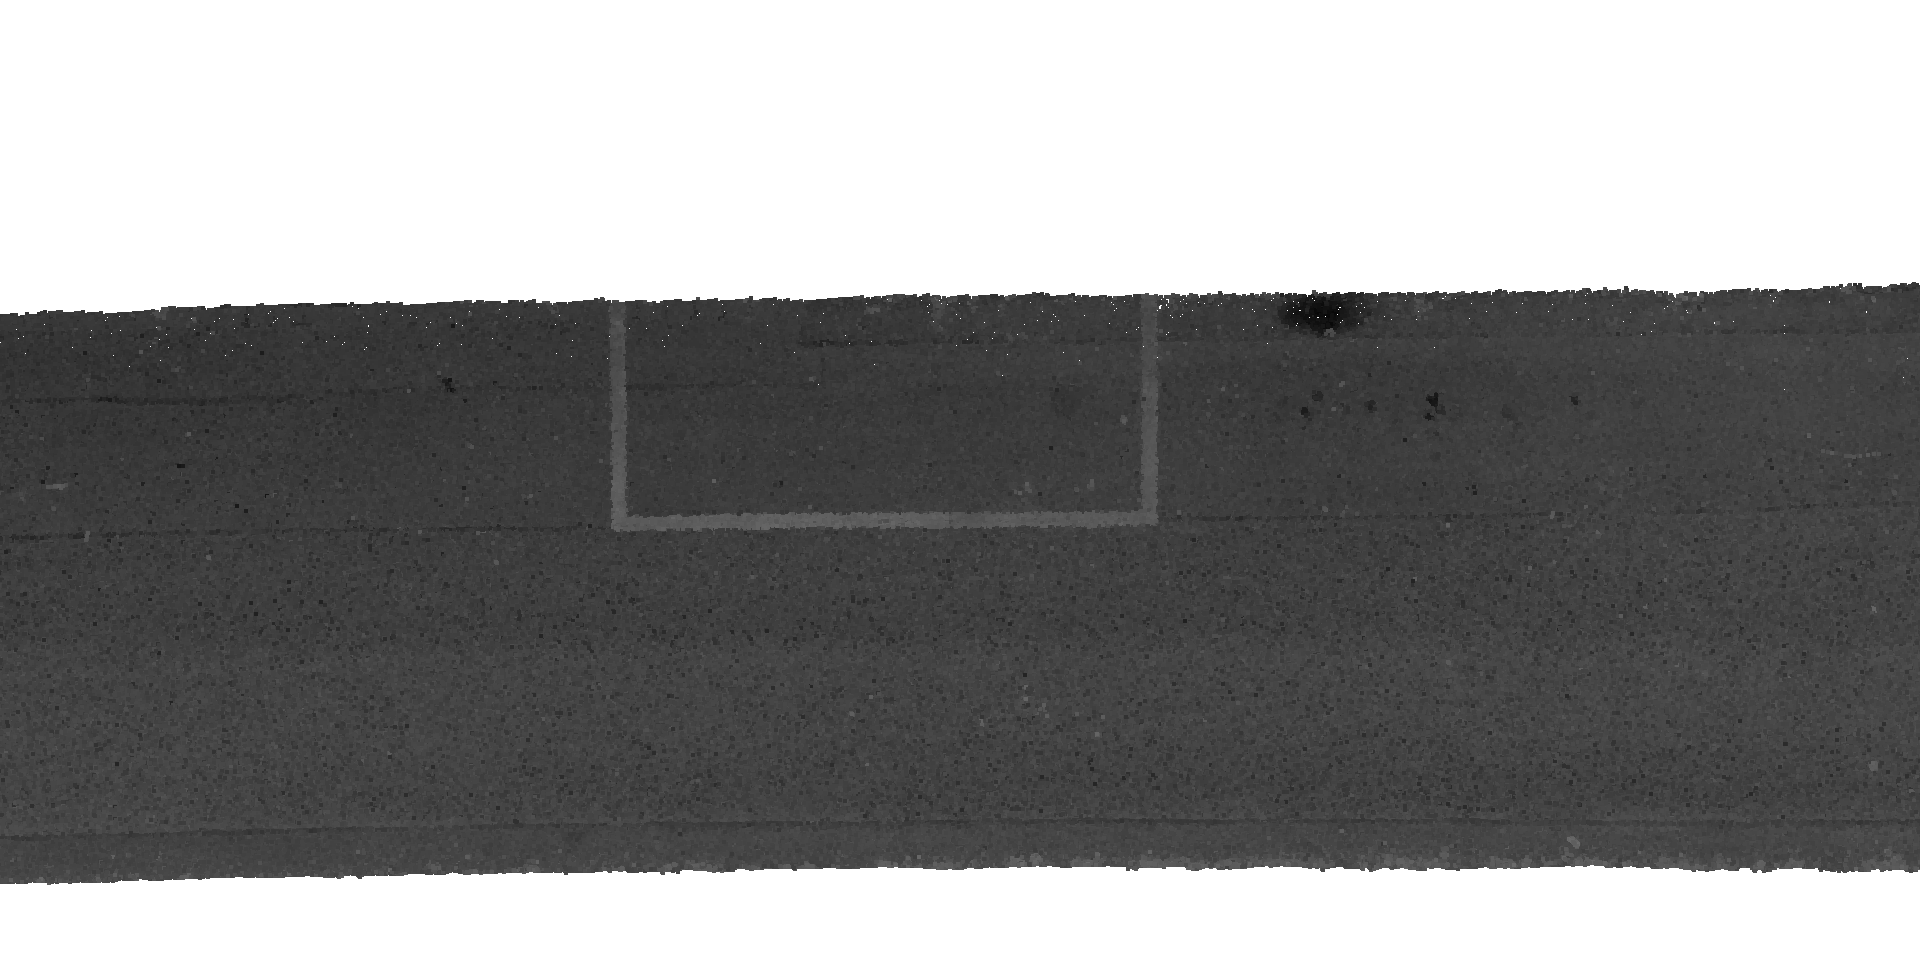
\includegraphics[width=0.48\textwidth]{graphics/eval_road_marking}}
    {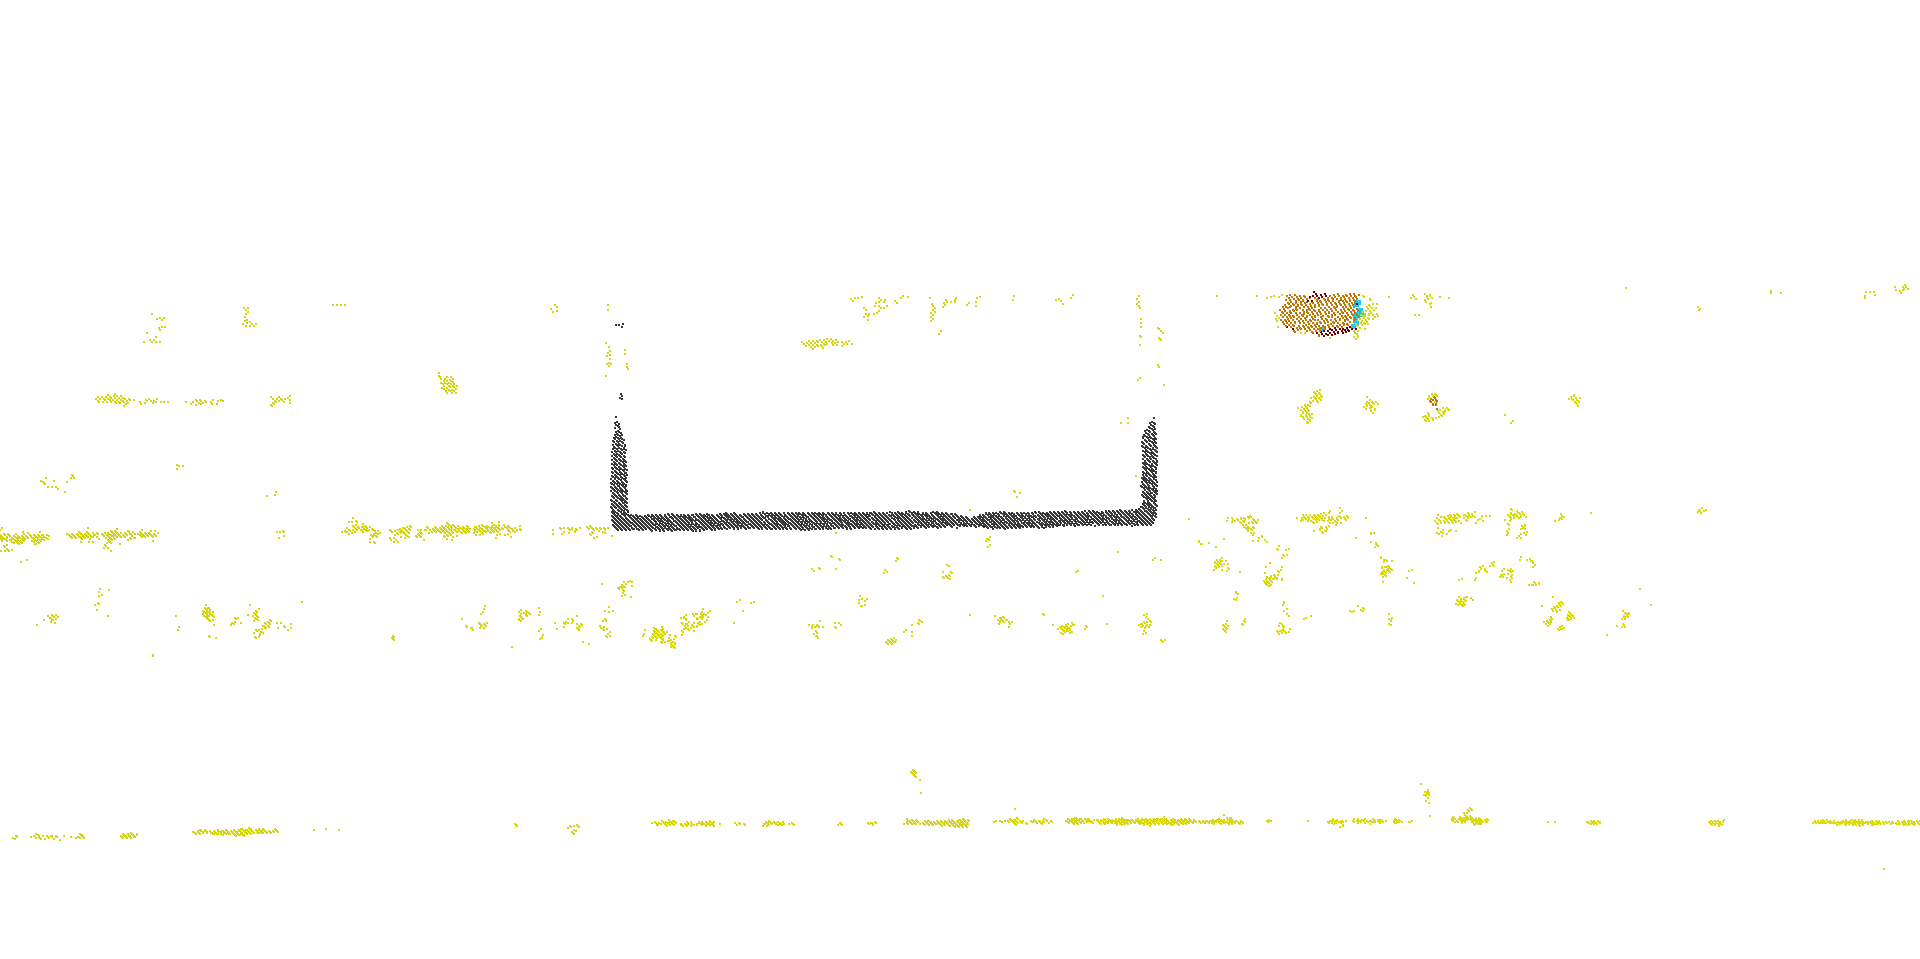
\includegraphics[width=0.48\textwidth]{graphics/eval_road_marking_classes}}
    \caption{Die Fahrbahnmarkierung in Intensität (links) und die Prediction davon (rechts).}
    \label{fig:road_marking}
\end{figure}

\begin{figure}
    {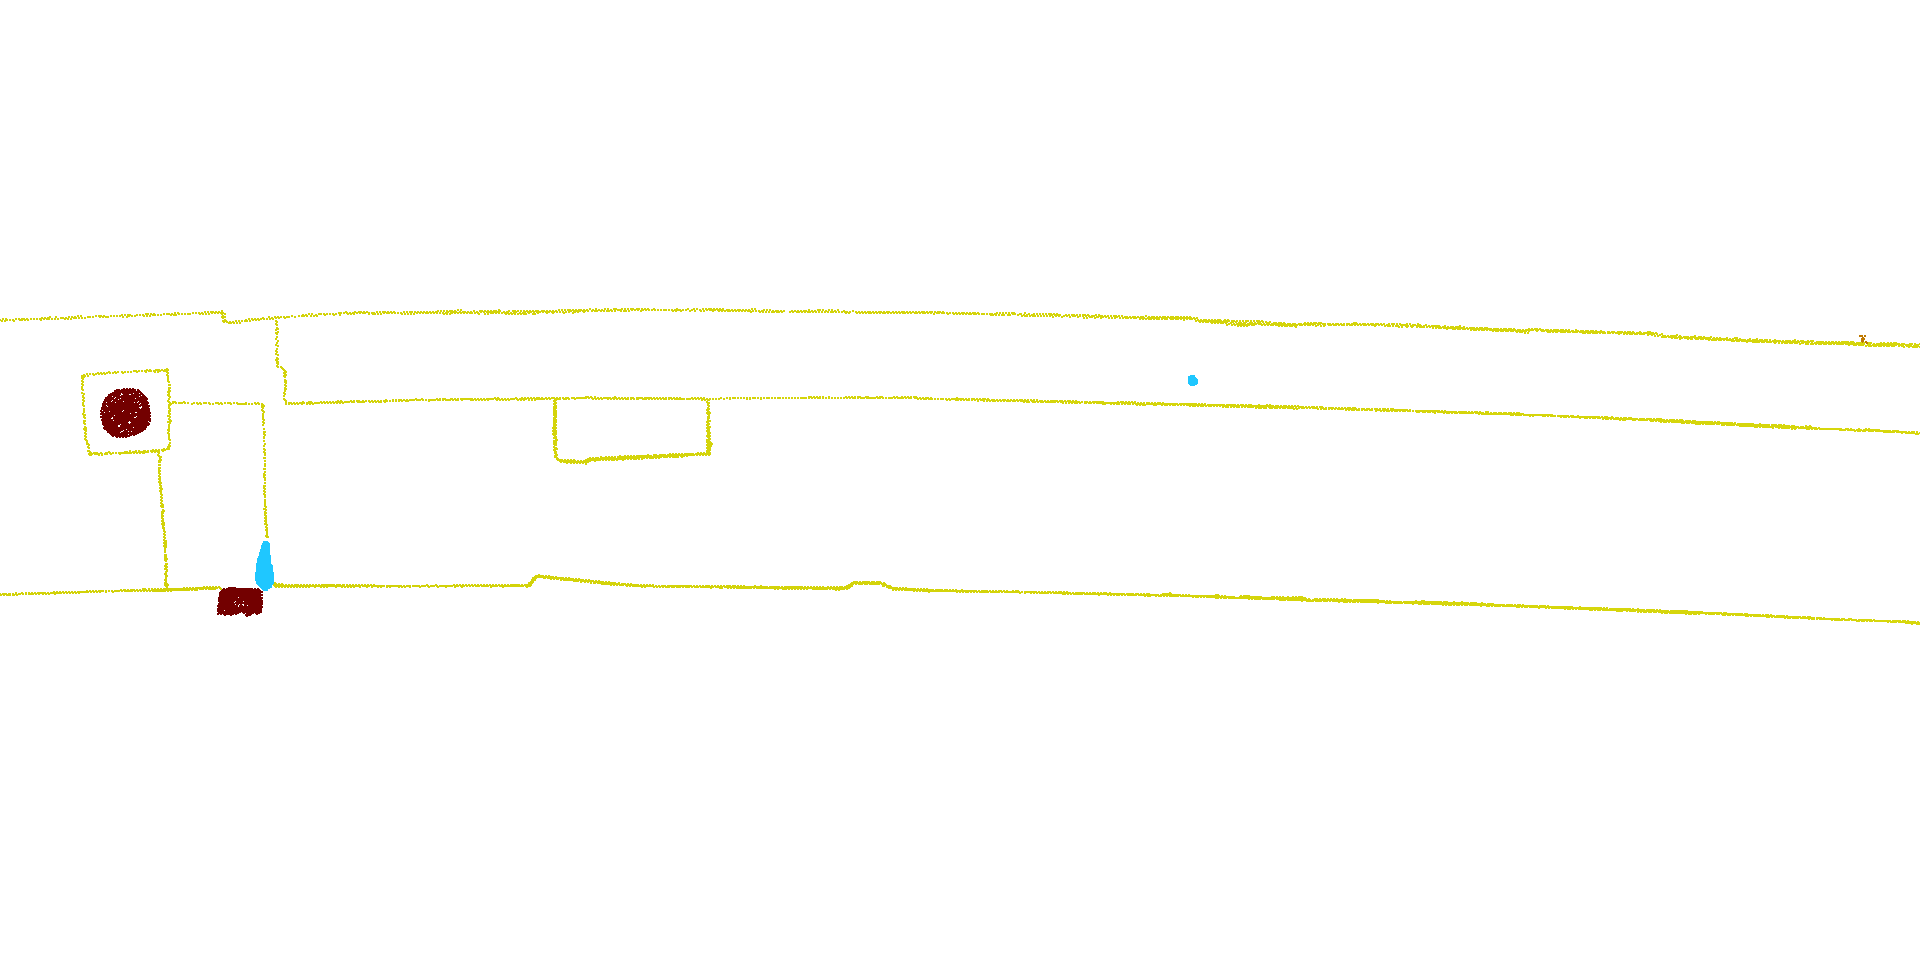
\includegraphics[width=0.96\textwidth]{graphics/eval_left_ground_truth}}
    \par\smallskip
    {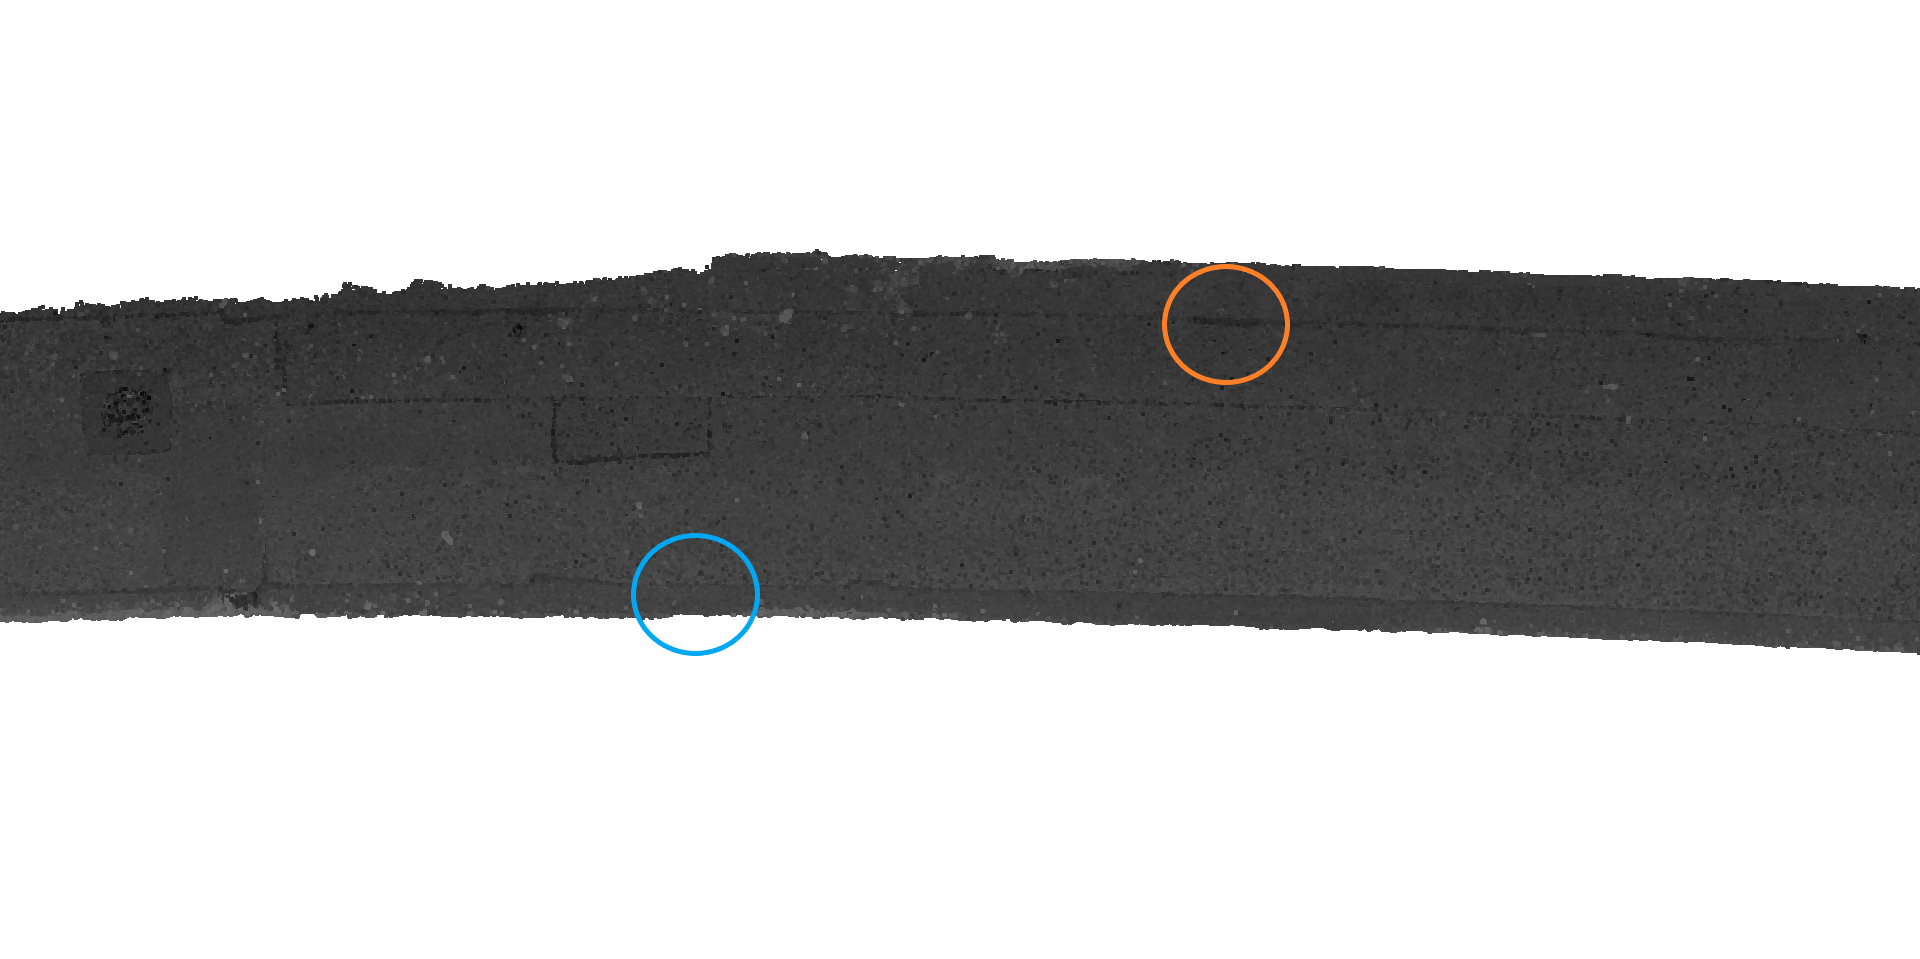
\includegraphics[width=0.96\textwidth]{graphics/eval_left_no_classes_circles}}
    \par\smallskip
    {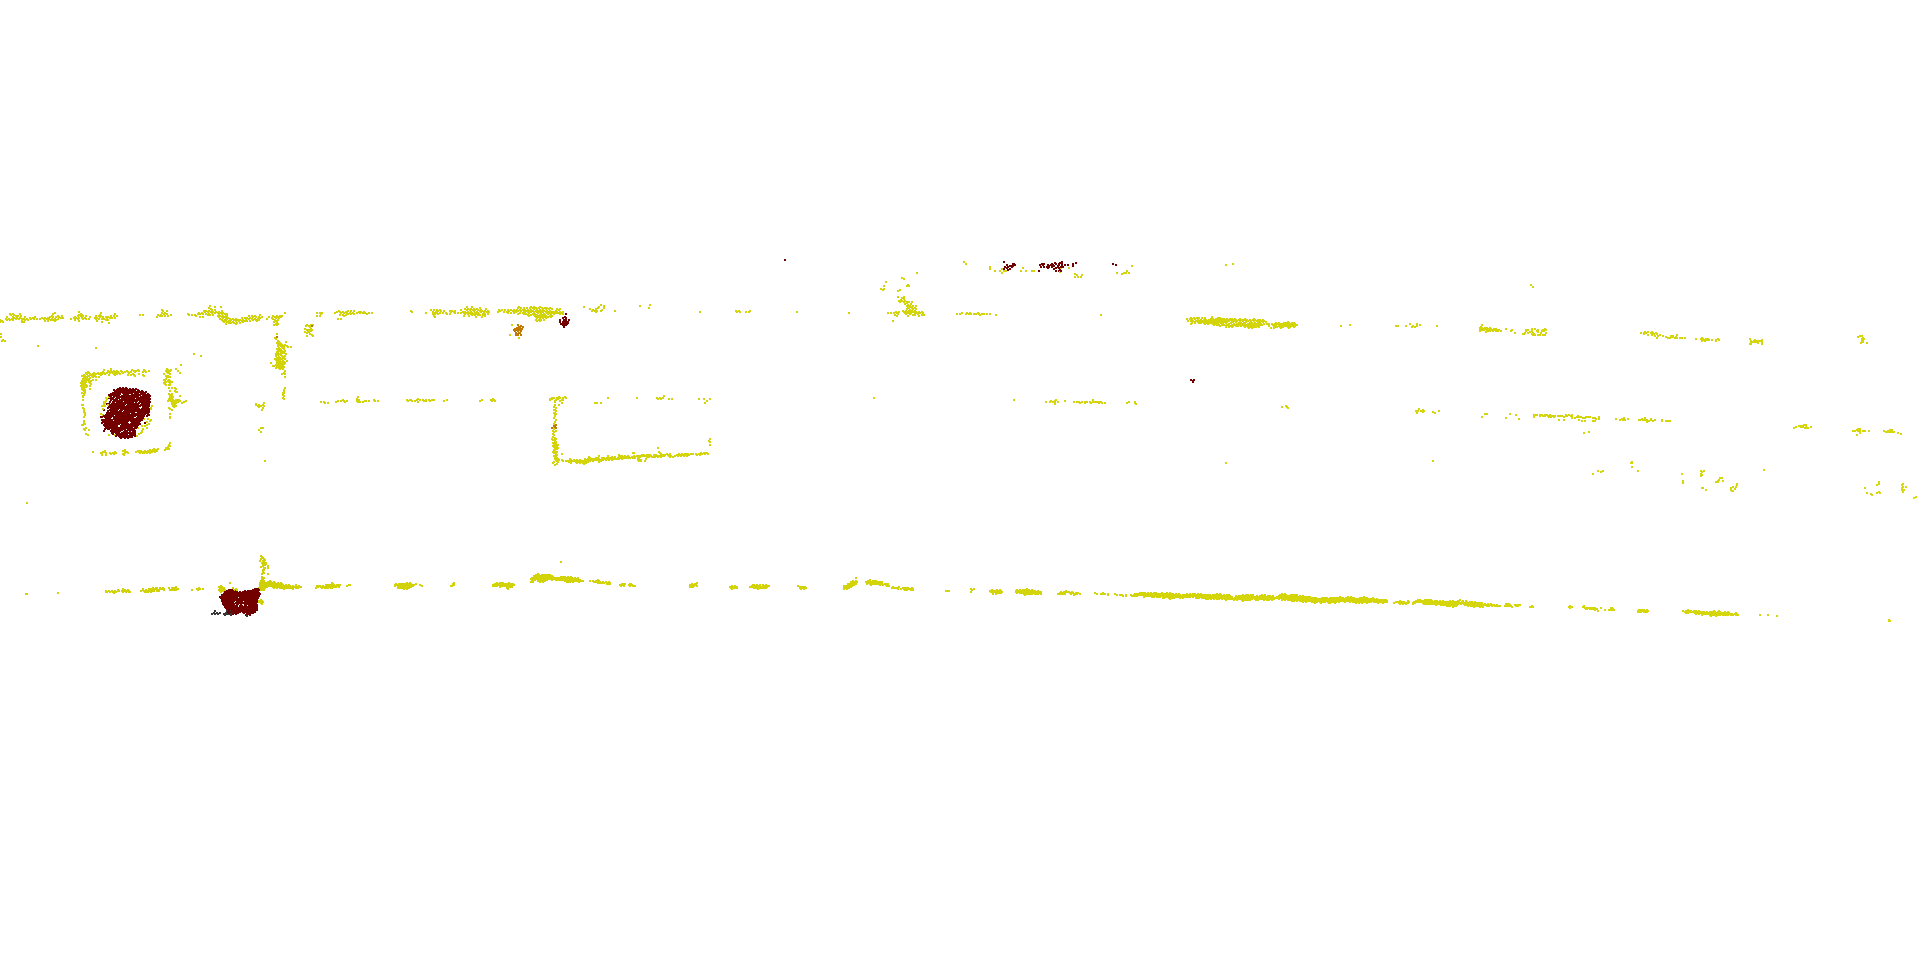
\includegraphics[width=0.96\textwidth]{graphics/eval_left_prediction}}
    \caption{Die tatsächlichen Klassen (oben), die Intensitäten der Punktwolke (mittig) und die Prediction von Flickstellen (unten). Der blaue Kreis markiert eine nicht erkannte Stelle, die kaum Intensitätsunterschiede aufweist. Der orange Kreis wiederum markiert eine Stelle, die übermäßig dick als Flickstelle klassifiziert wird und einen breiten, in der Intensität auffälligen Streifen bildet.}
    \label{fig:cmp_flickstellen}
\end{figure}

\begin{figure}
    {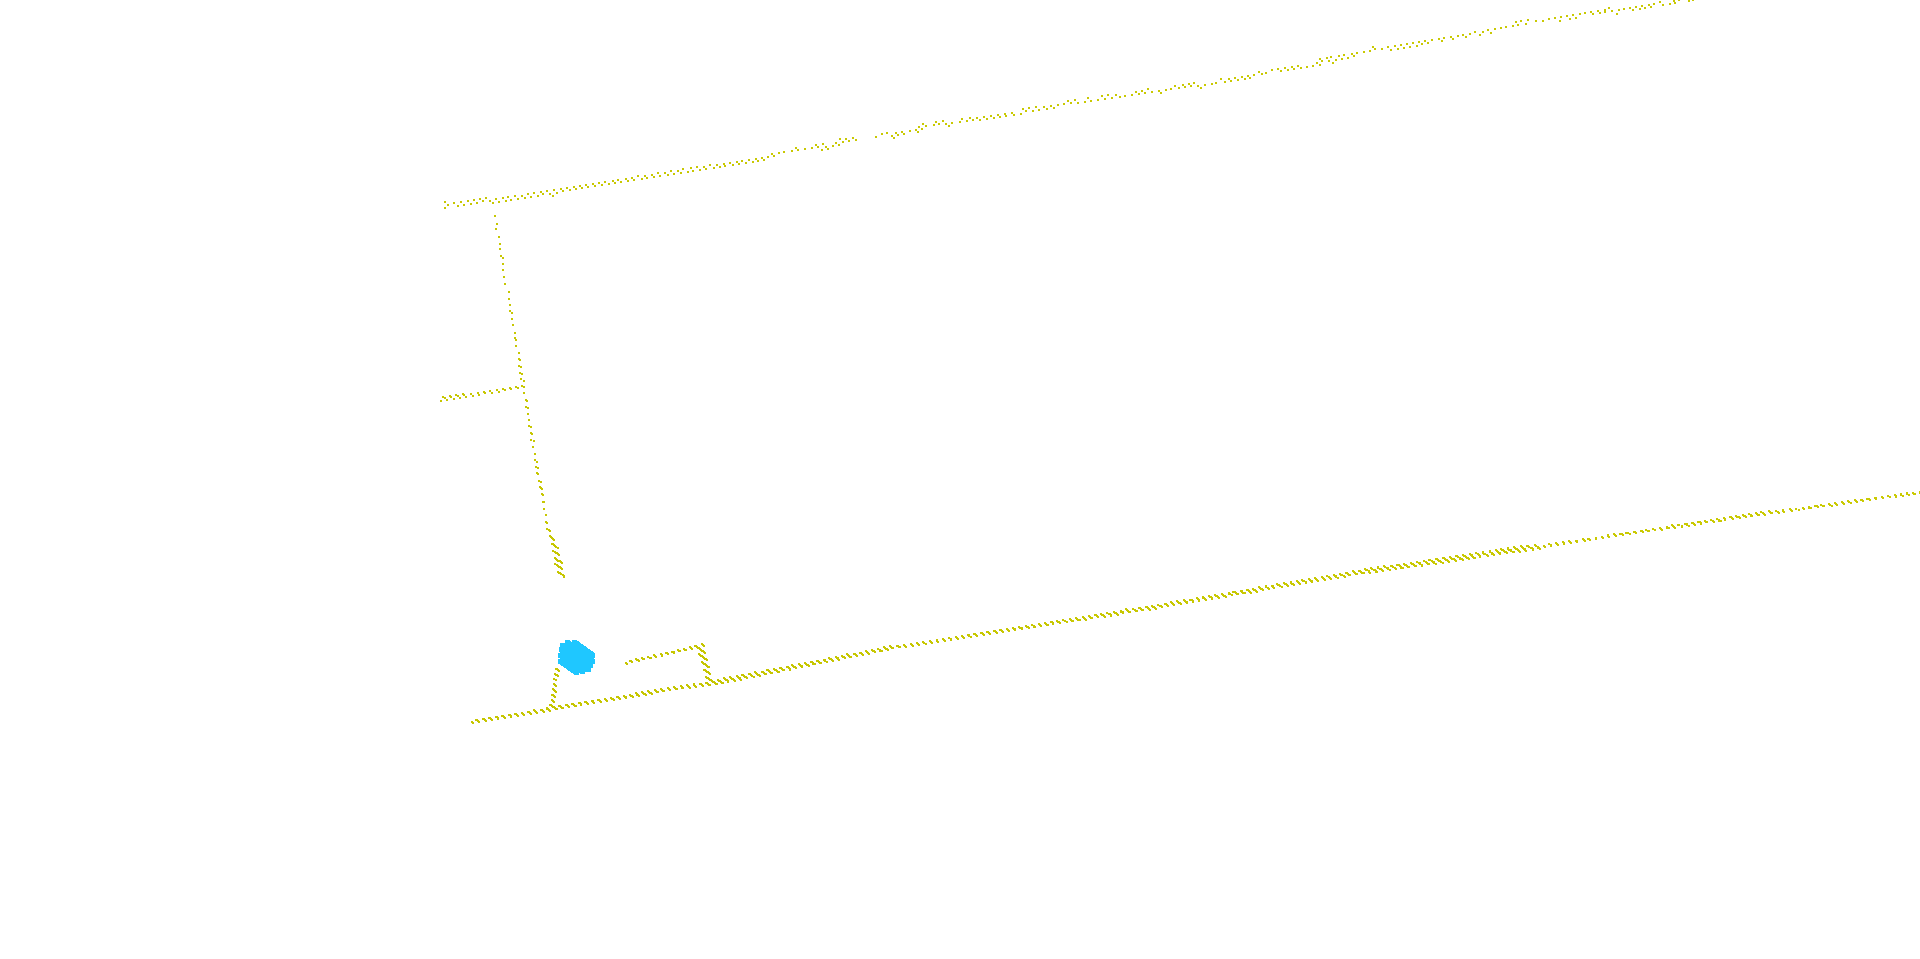
\includegraphics[width=0.96\textwidth]{graphics/eval_flickstelle_pothole_ground_truth}}
    \par\smallskip
    {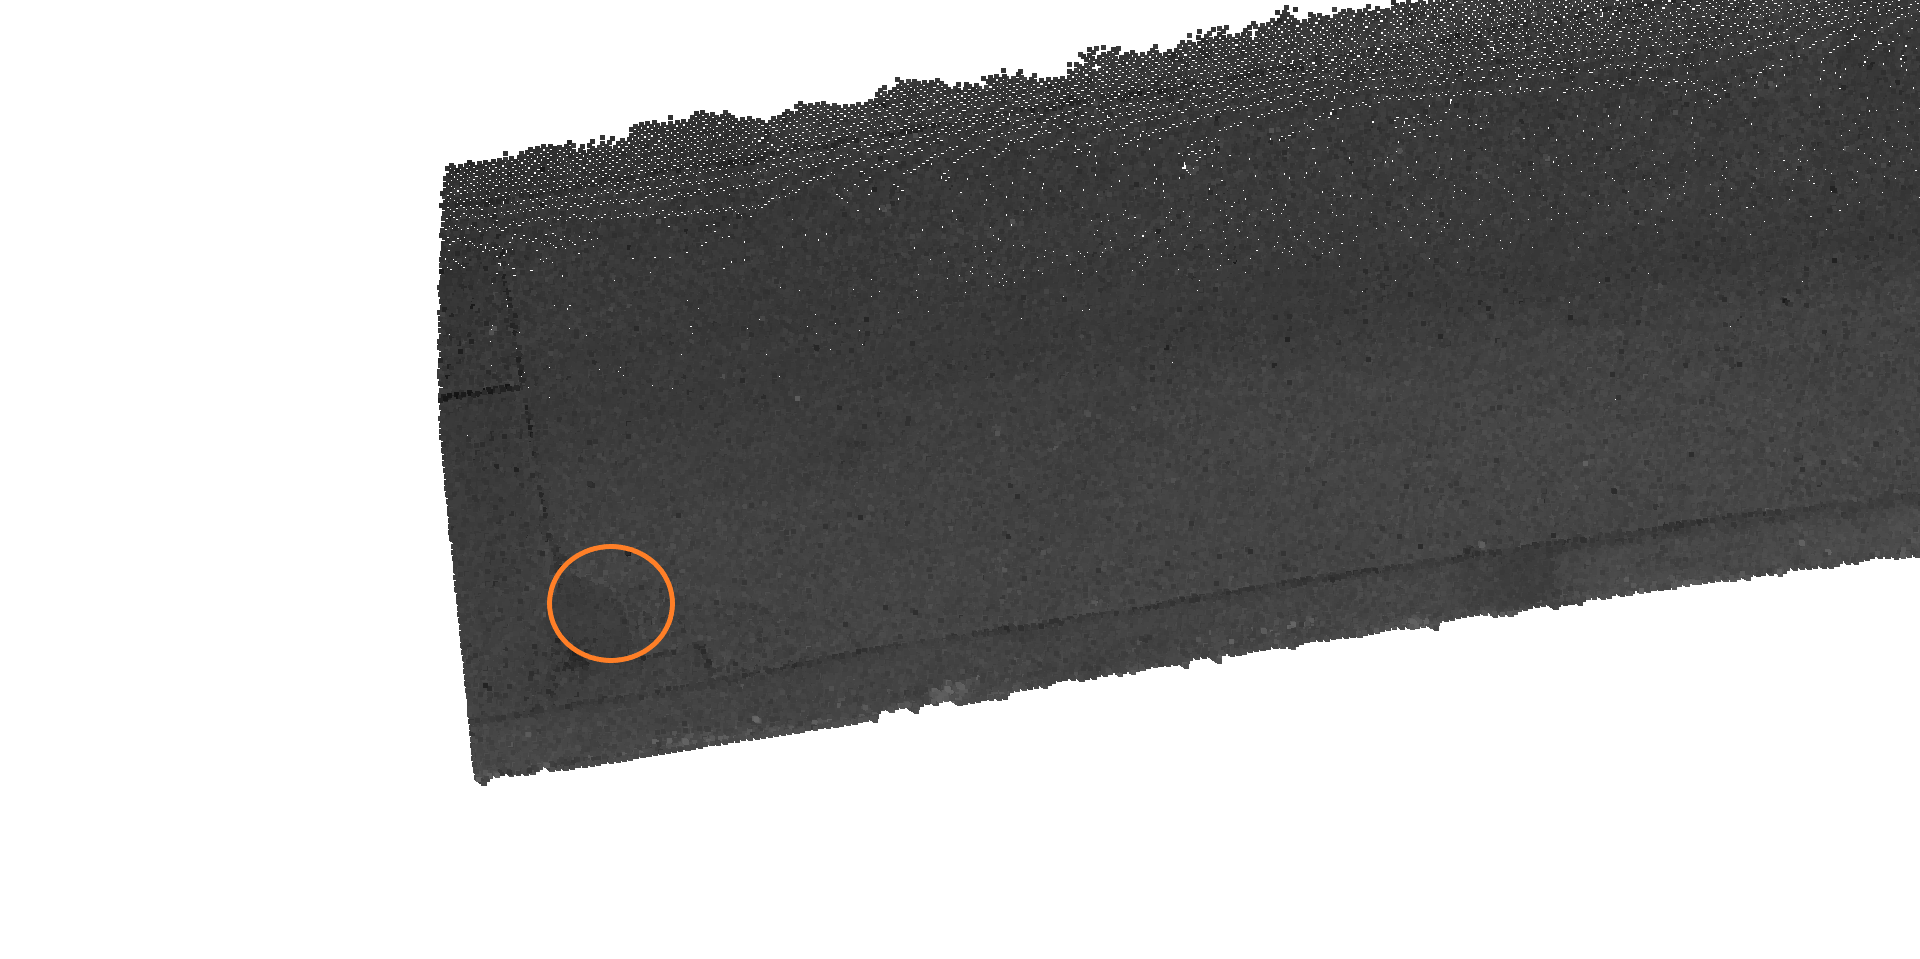
\includegraphics[width=0.96\textwidth]{graphics/eval_flickstelle_pothole_no_classes_circles}}
    \par\smallskip
    {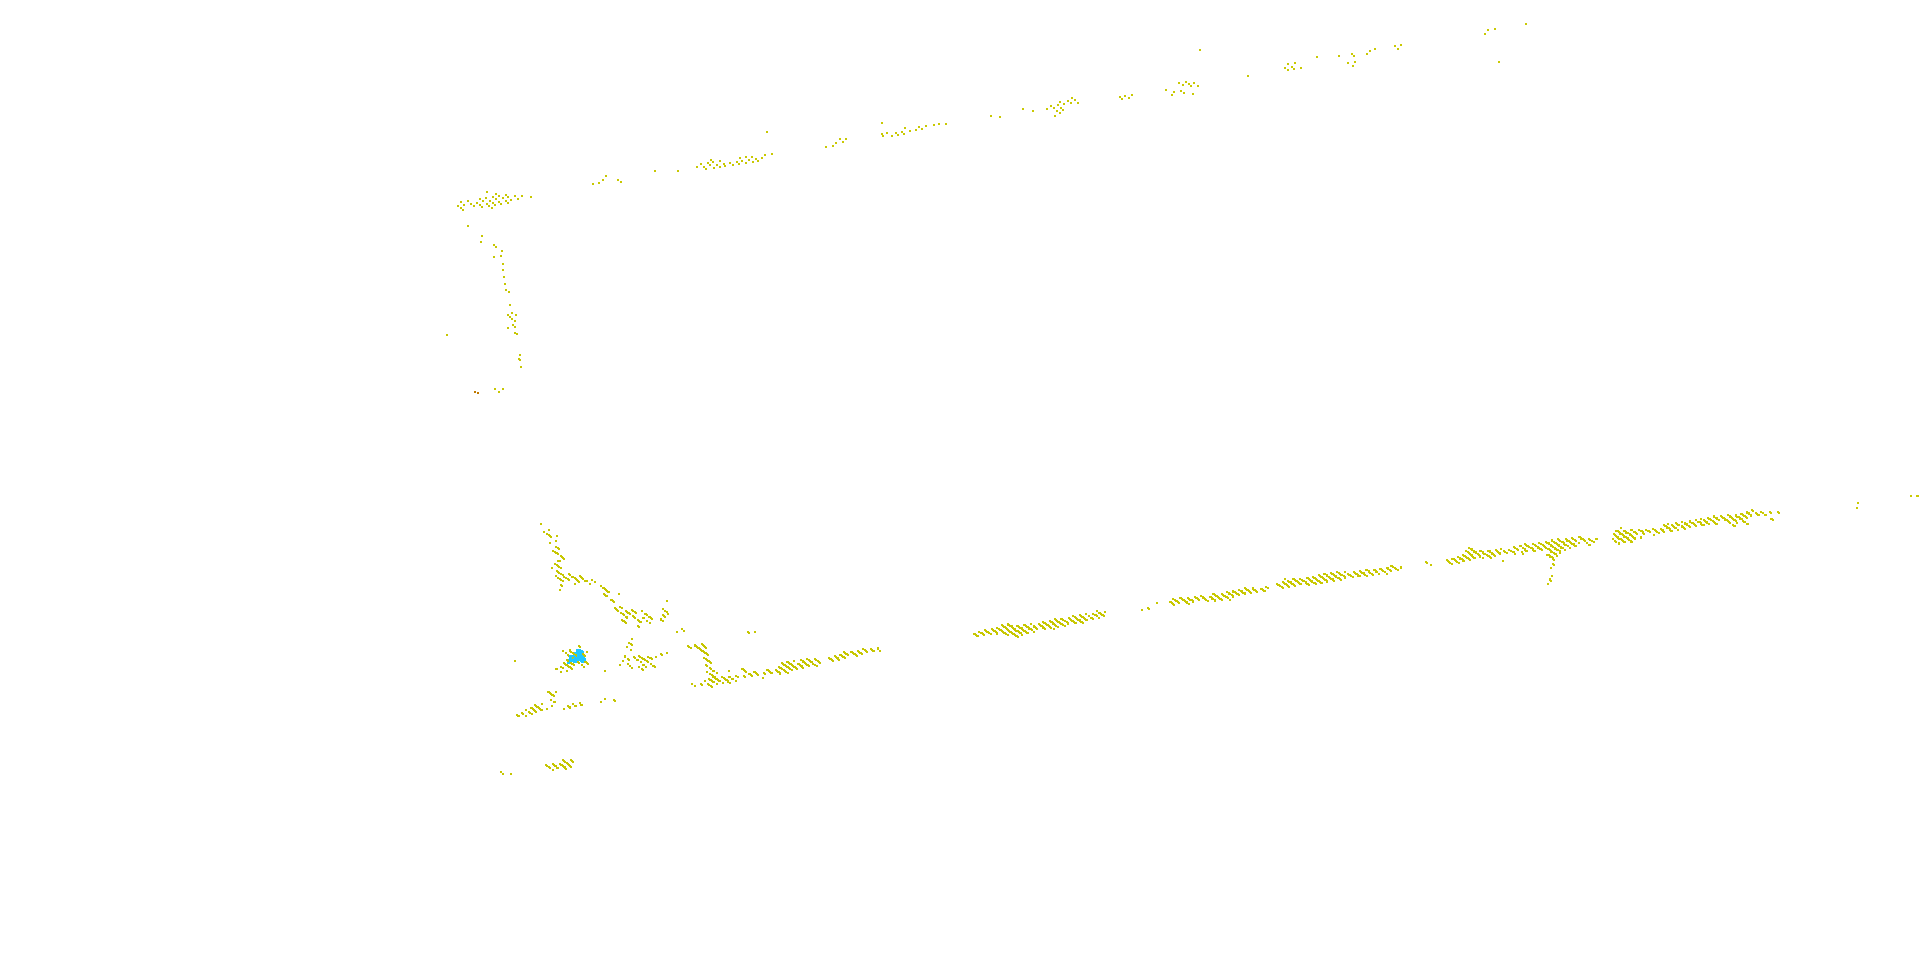
\includegraphics[width=0.96\textwidth]{graphics/eval_flickstelle_pothole_prediction}}
    \caption{Die tatsächlichen Klassen (oben), die Intensitäten der Punktwolke (mittig) und die Prediction (unten). Zu erkennen ist eine vom Modell ergänzte Flickstelle.}
    \label{fig:new_flickstelle}
\end{figure}

\begin{figure}
    {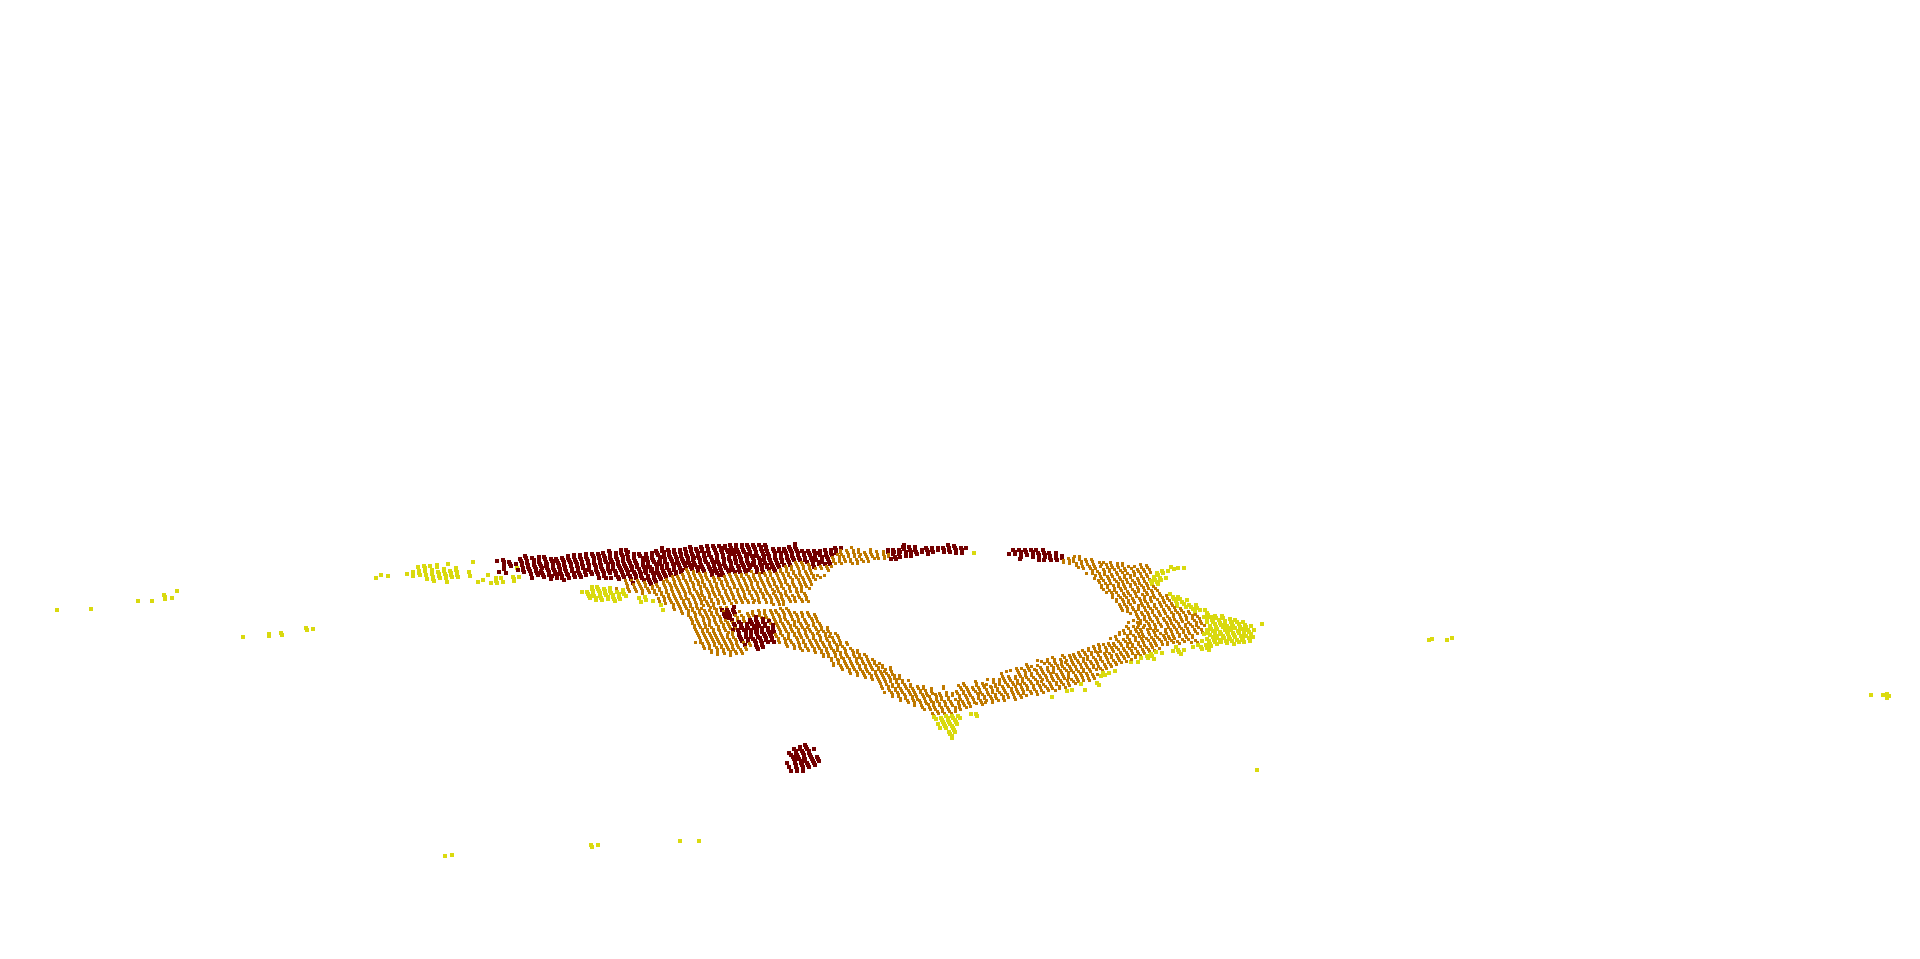
\includegraphics[width=0.6\textwidth]{graphics/eval_gully_misclas}}
    {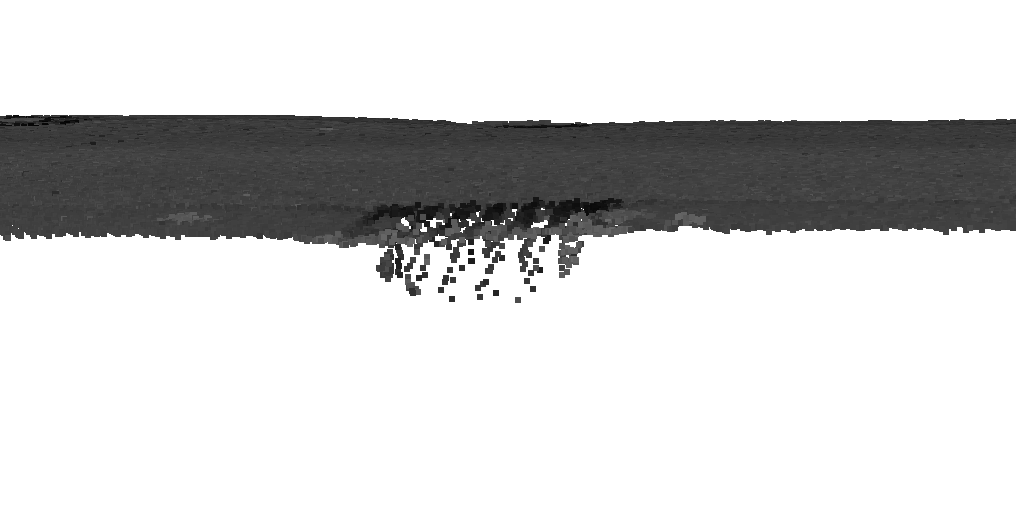
\includegraphics[width=0.36\textwidth]{graphics/low_gully_points}}
    \caption{Einige in rot gefärbte Fehlklassifzierungen als Gully (links) und niedrig gelegene Punkte bei einem kleinen Gully (rechts).}
    \label{fig:gully_misclas}
\end{figure}

\subsection{Vergleich mit nur einwertigen Features}

An dieser Stelle sollen die Ergebnisse eines Experiments vorgestellt werden, das lediglich einwertige Features nutzt und davon 8 pro Scale. Diese Features orientieren sich an den mehrwertigen des Basisexperiments und sind 
\begin{itemize}
    \item Durchschnitt und Standardabweichung der umgebenden Intensität \citep{Li.Cheng-2018}
    \item die durchschnittliche Intensitätsdifferenz zum Ursprungspunkt
    \item der durchschnittliche Höhenunterschied, gemessen anhand der Differenz der \textit{z}-Koordinaten
    \item die vier vorgestellten Eigenwert-basierten Features \textit{Linearity}, \textit{Planarity}, \textit{Scattering} sowie \textit{Curvature}.
\end{itemize}
Die genutzten Scales sind dieselben wie für das Basisexperiment. Der einzige weitere Unterschied ist die maximale Baumtiefe beim \textit{Random Forest}, die hier bei 8 statt 15 liegt, da die Größe der Featurevektoren deutlich kleiner ist (40 statt 240). Aus diesem Grund verbessert sich auch die Performance im Vergleich zum Basisexperiment: Die gesamte Laufzeit ist mit knapp 180$s$ um 30$s$ geringer, was sich insbesondere mit der kleineren Größe von 240 MB der zu schreibenden und zu lesenden Featuresdatei erklären lässt. Auch das Training verschnellert sich wegen der kleineren Featurevektoren und Baumtiefen auf 15$s$. Der maximale Speicherverbrauch liegt 0,8 GB. \\
Die Metriken zur \textit{Prediction} des Versuchs finden sich in Tabelle \ref{table:absolute_value_metrics}. Sie sind tendenziell etwas niedriger, aber unterscheiden sich grundsätzlich nicht stark von denen des Basisexperiments. Die Ölflecken werden sogar, wohl wegen ihrer extrem geringen Intensität, leicht besser erkannt. Wie in Abbildung \ref{fig:cmp_absolute_full} zu sehen, ähnelt auch die Klassifikation der Flickstellen der vom Basisexperiment. Allerdings sind sowohl \textit{Precision} als auch \textit{Recall} geringer und es ist ein stärkeres Rauschen in der Klassifikation erkennbar um die Fahrbahnmarkierung herum. Die Histogramme des Basisexperiments scheinen also tatsächlich besser mit solch wenigen Außenseiterpunkten umgehen und Rauschen vermindern zu können. \\
Aus Abbildung \ref{fig:cmp_absolute_detail} lassen sich zwei weitere Erkenntnisse gewinnen: Die planare Mitte der Gullys wird in diesem Experiment deutlich schlechter und vollständig als gewöhnliche Straße klassifiziert. Hintergrund dafür ist wahrscheinlich, dass die Scales nicht ausreichend groß sind, um auffälligere Punkte des Gullys zu erreichen. Maße wie \textit{Curvature} sind entsprechend besonders niedrig. Histogramme von nachbarschaftsbasierten Features, wie es \textit{Curvature} ist, können diese Begrenzung etwas aufweichen: Die \textit{Curvature}-Werte derjenigen Punkte der Gullymitte, die ein wenig näher am Rand und damit den auffälligeren Punkten liegen, sind entsprechend höher. Sofern sie noch im Scale des Ursprungspunkts liegen, fließen diese Werte auch in das Histogramm ein, welches damit effektiv einen deutlich größeren Scale abdeckt. \\
Des Weiteren sind Schlaglöcher schwerlich mit (zumindest den hier genutzten) einwertigen Features zu erkennen. Stattdessen werden die Punkte dieser Klasse häufig als Gully oder Flickstelle klassifiziert. Die Ursache liegt vermutlich in den lokal teils ähnlichen Formen von Gullypunkten bzw. den zu Flickstellen vergleichbaren Intensitätsunterschieden zur Nachbarschaft. Die genauere Charakterisierung der Nachbarschaft und damit größere Unterscheidungskraft zu anderen Klassen kann durch Nutzung mehrwertiger Features erreicht werden. Zwar ist der Speicherverbrauch deutlich und die Laufzeit etwas geringer mit einwertigen Features, doch werden insbesondere wegen der - für diesen Anwendungsfall wichtigen - besseren Erkennung von Schlaglöchern weiterhin Histogramme verwendet.

\begin{table}
\centering
\begin{tabular}{c|c|c|c|c|c|c}
 & \textit{U} & \textit{S} & \textit{F} & \textit{G} & \textit{Ö} & \textit{M} \\
\hline
Precision & 0,988 & 0,462 & 0,369 & 0,703 & 0,974 & 0,941 \\
Recall    & 0,992 & 0,018 & 0,302 & 0,770 & 0,760 & 0,608 \\
F1        & 0,990 & 0,034 & 0,332 & 0,735 & 0,853 & 0,739 \\
\end{tabular}
\caption{Die Metriken der einzelnen Klassen für das Experiment mit nur einwertigen Features.}
\label{table:absolute_value_metrics}
\end{table}

\begin{figure}
    {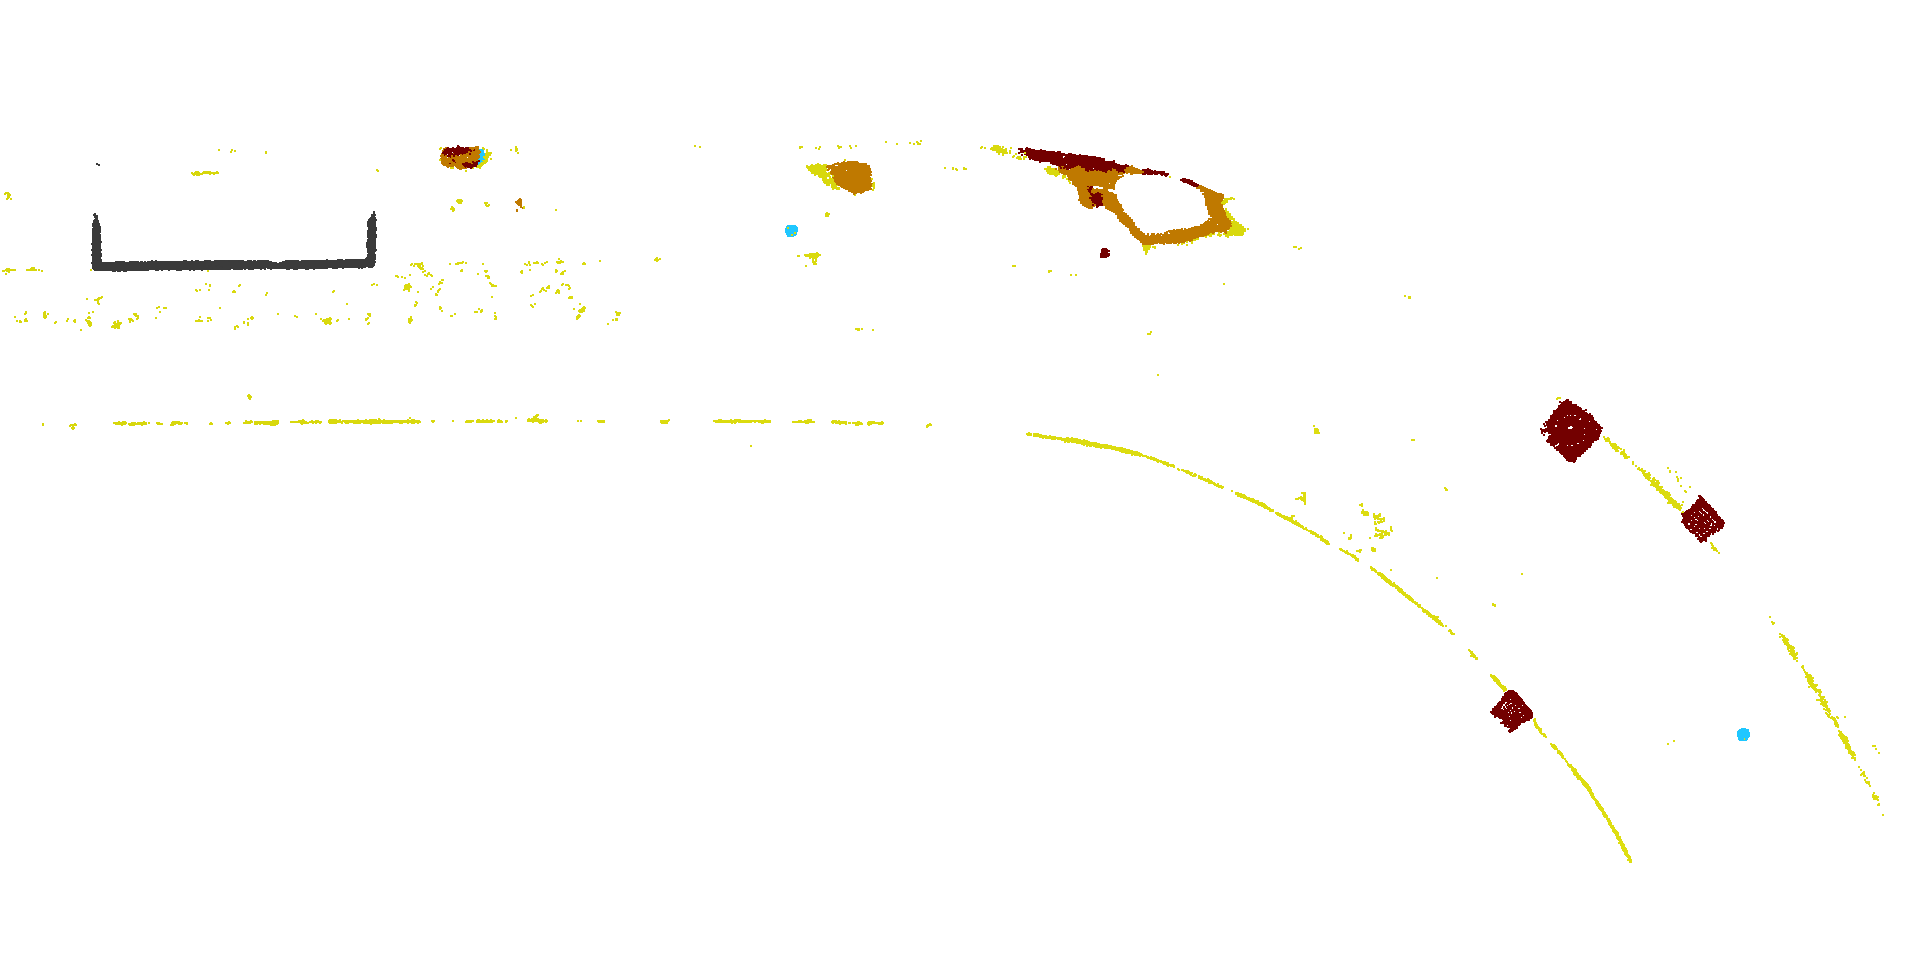
\includegraphics[width=0.95\textwidth]{graphics/eval_right_prediction}}
    \par\smallskip
    {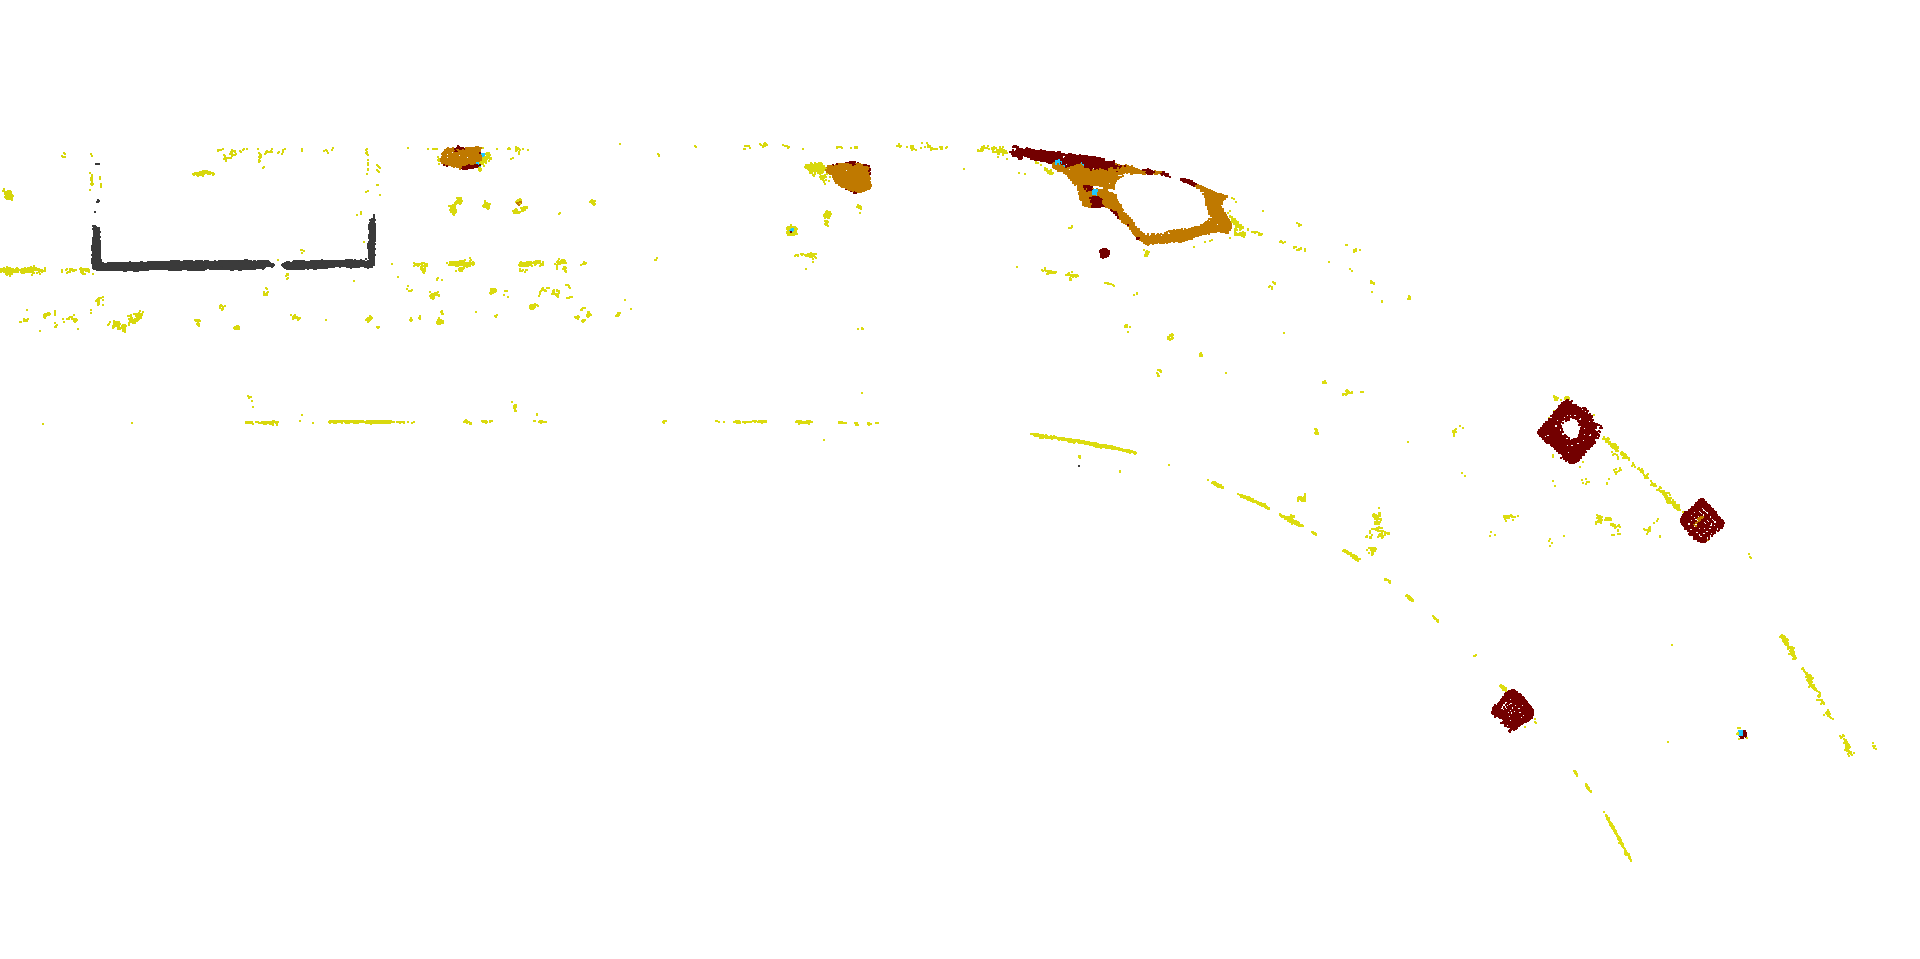
\includegraphics[width=0.95\textwidth]{graphics/eval_right_absolute}}
    \caption{Die Prediction mit mehrwertigen Features (oben) und mit einwertigen (unten).}
    \label{fig:cmp_absolute_full}
\end{figure}

\begin{figure}
    {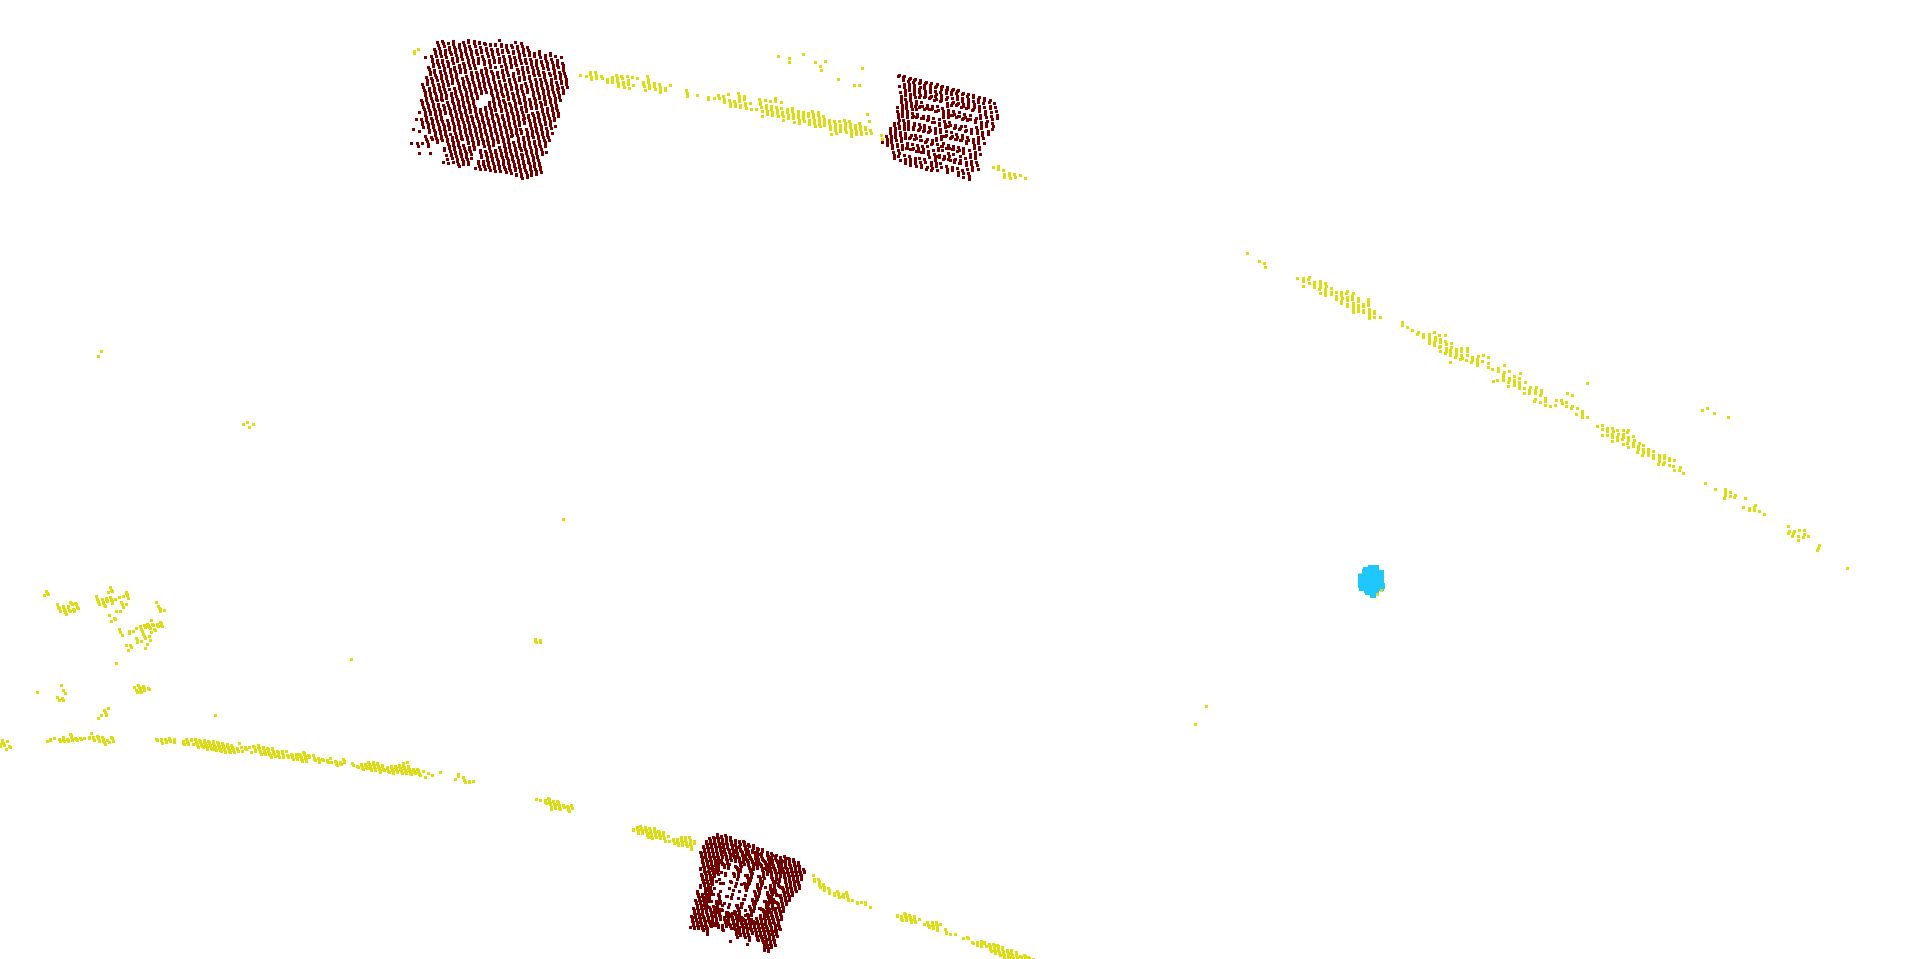
\includegraphics[width=0.48\textwidth]{graphics/eval_gully_pothole_prediction}}
    {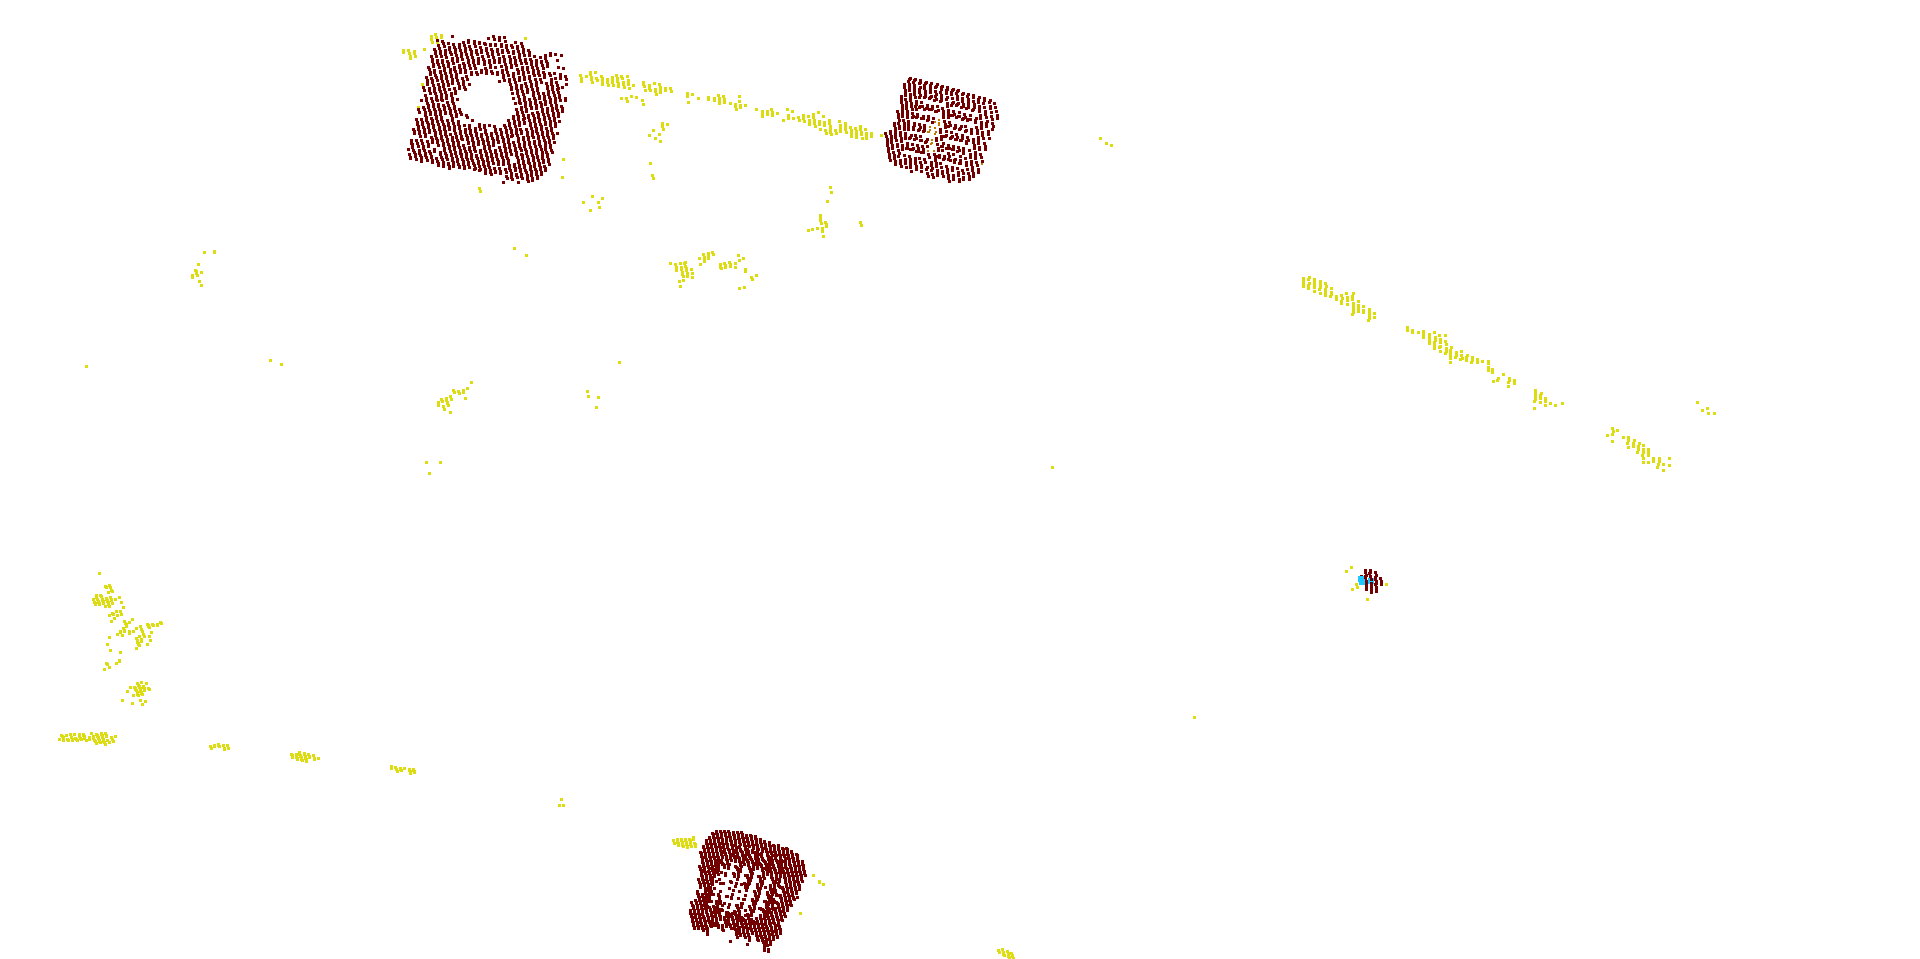
\includegraphics[width=0.48\textwidth]{graphics/eval_gully_pothole_absolute}}
    \caption{Die Prediction von Gullys und Schlaglöchern mit mehrwertigen Features (links) und mit einwertigen (rechts).}
    \label{fig:cmp_absolute_detail}
\end{figure}

\subsection{Vergleich mit größeren Scales}

Scales über 15$cm$ werden standardmäßig nicht verwendet, doch besteht die Möglichkeit ihrer Nutzung, wenn etwa größere Objekte zu detektieren sind. Für diesen Ansatz werden dann nach Dichtereduktion der Punktwolke die Featurevektoren der Punkte approximiert. Ein Vergleich der Laufzeiten für einzelne Scales mit und ohne Approximation auf der Testpunktwolke findet sich in Tabelle \ref{table:bigger_scales}. Die Werte der \textit{Half Edge Length} reichen dabei von 0,75$cm$ bis zu 1,5$cm$, was zu einer Reduktion um 24\% bis zu 64\% der Punktmenge führt. Aus den Daten wird deutlich, dass dieses Prinzip eine große zeitliche Ersparnis bringt. Die Stärke der Dichtereduktion ist im Sinne guter Ergebnisse jedoch auch begrenzt: Eine \textit{Half Edge Length} von 2$cm$ zum Beispiel reduziert bereits die Punktmenge um knapp 80\%. Ob aus einer so geringen oder noch geringeren Zahl an Punkten aussagekräftige Features extrahiert werden können, ist fraglich. \\ 

\begin{table}
\centering
\begin{tabular}{c|c|c|c|c|c}
Approximation & 20$cm$ & 25$cm$ & 30$cm$ & 40$cm$ & 50$cm$ \\
\hline
ja   & 83$s$ & 102$s$ & 113$s$ & 120$s$ & 102$s$ \\
nein & 132$s$ & 203$s$ & 292$s$ & 516$s$ & 802$s$ \\
\end{tabular}
\caption{Die Dauer der Feature Extraction für unterschiedliche größere Scales, mit und ohne Approximation der Featurevektoren.}
\label{table:bigger_scales}
\end{table}

Der Nutzen und die Qualität der Approximationen soll getestet werden, indem das Basisexperiment erweitert wird um den größeren Scale von 25$cm$. Dies sorgt wie erwartbar für eine erhöhte Laufzeit sowohl bei der Featureberechnung als auch dem \textit{Prediction}-Prozess sowie für einen größeren Speicherverbrauch während der Verarbeitung und in Form der Featuresdatei. Wegen der größeren Featurevektoren wird die maximale Baumtiefe auf 20 gesetzt. \\
Auf die Metriken hat der zusätzliche Scale kaum einen Einfluss. Es wird allerdings die Vermutung bestätigt, dass der größere Scale auch für eine bessere Erkennung größerer Objekte sorgt (Abbildung \ref{fig:cmp_bigger_scale}). Das Innere des Gullys, das bereits im Basisexperiment weitgehend erkannt wurde, wird nun vollständig korrekt als Gully klassifiziert. Ähnliches gilt für das nahegelegene Schlagloch, das nun einen etwas größeren Radius umfasst. Der größere Scale sorgt dafür, dass zum Beispiel bei den äußeren Schlaglochpunkten nun die charakteristischen Vertiefungen stärker erfasst werden und die Klassifizierung als Schlagloch somit erleichtert oder erst ermöglicht wird. \\
Auf die zuvor gar nicht erkannten Schlaglöcher oder Flickstellen hat der größere Scale keinen Einfluss, was dafür spricht, dass dies tatsächlich mit den genutzten und nicht genügend aussagekräftigen Features in Verbindung steht. Größere Scales können also für - zumindest auf den gegebenen Daten - kleine Verbesserungen sorgen. Mit Blick auf den dadurch gestiegenen Ressourcenverbrauch werden diese Scales zunächst dennoch nicht verwendet für die \textit{Predictions}. Für dezidierte Anwendungsfälle wie der vollständigen Erkennung von Gullys oder bei Straßen in deutlich schlechterem Zustand könnte dieser Schritt aber sinnvoll sein.

\begin{figure}
    {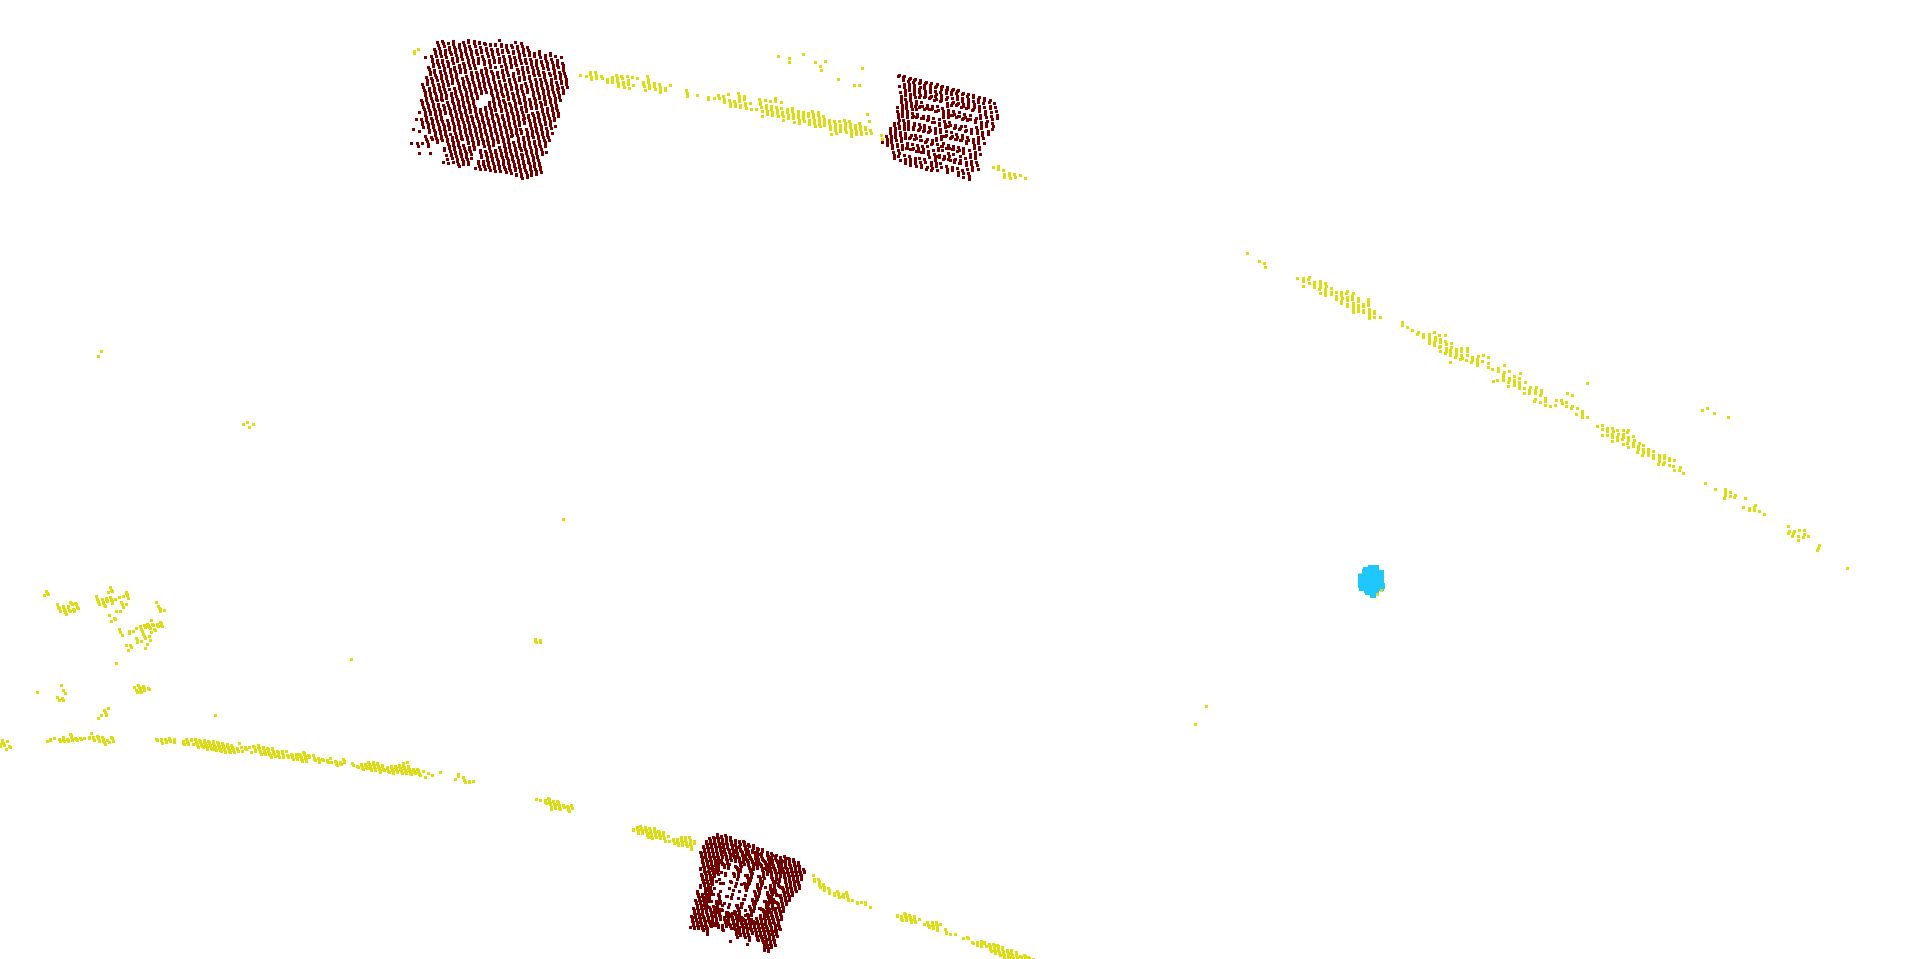
\includegraphics[width=0.48\textwidth]{graphics/eval_gully_pothole_prediction}}
    {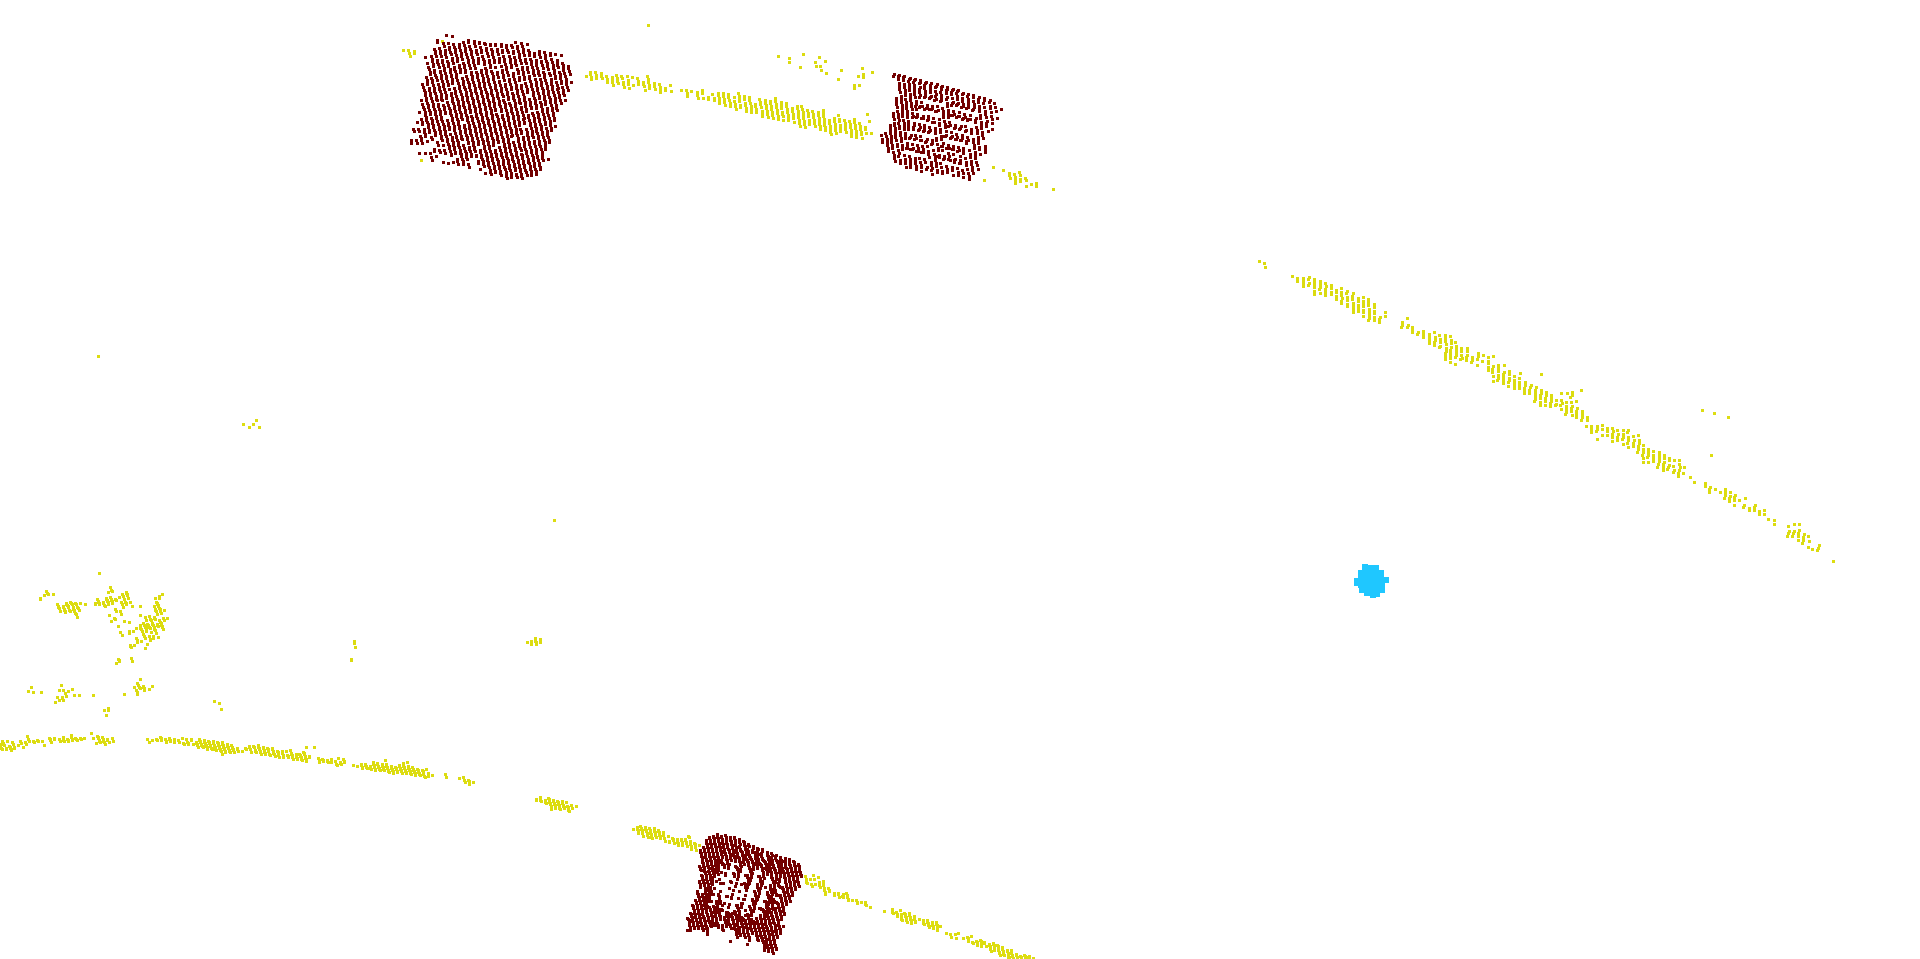
\includegraphics[width=0.48\textwidth]{graphics/eval_gully_pothole_bigger_scale}}
    \caption{Die Prediction von Gullys und Schlaglöchern ohne größeren Scale (links) und mit (rechts).}
    \label{fig:cmp_bigger_scale}
\end{figure}

\subsection{Uniqueness}

Mittels des \textit{Uniqueness}-Konzepts soll die Menge der zur \textit{Prediction} an das Modell übergebenen Punkte reduziert werden. Das Ziel ist dabei, möglichst wenig der gewöhnlichen Straßenpunkte als \textit{unique} zu erkennen und dafür möglichst viele der Punkte der anderen Klassen. In Tabelle \ref{table:alphas} sind die Anteile als \textit{unique} erkannter Punkte pro Klasse dokumentiert, wobei jeweils verschiedene $\alpha$-Werte genutzt wurden, die tendenziell die Größe der übrig gebliebenen Menge bestimmen. \\
Dabei ist zu beobachten, dass der Anteil der Straßenpunkte mit höherem $\alpha$ schnell sinkt. Für die Flickstellen gilt Ähnliches, wenn auch auf geringerem Niveau. Dies spricht erneut dafür, dass die Features nicht so aussagekräftig für Flickstellen sind wie für Gullys oder Schlaglöcher. Allerdings gilt dabei, wie in Abbildung \ref{fig:cmp_uniqueness} zu sehen, dass die nicht als \textit{unique} erkannten Flickstellen ohnehin meist solche sind, die nicht oder nur schwach korrekt vom Modell klassifiziert werden. Somit hätte ihre Nichtbeachtung für die \textit{Prediction} geringe Auswirkungen auf die Qualität des Ergebnisses. \\
Mit $\alpha = 3,0$ wird bereits eine Reduktion um 88\% erreicht. Wenn diese etwas vorsichtiger ausfallen und beispielsweise alle Schlaglöcher enthalten soll, kann noch immer $\alpha = 2,0$ gesetzt werden und eine Reduktion um 75\% stattfinden. Solange der \textit{Feature-Extraction}-Ansatz nicht auf vielen weiteren Punktwolken getestet wurde, wird für den Einsatz der Schadenserkennung $\alpha = 0$ gesetzt, um möglichst keine bedeutsamen Klassen auszulassen bei der \textit{Prediction} und dennoch eine kleine Reduktion von 15\% zu erzielen. Wenn der Anwendungszweck die Registrierung von Punktwolken ist, kann mit einem deutlich höheren $\alpha$ gearbeitet werden: Die Gullys werden auch dann, bis auf ihre mittigen planaren Stellen, als \textit{unique} erkannt und charakterisieren die Straße mit nur wenigen Punkten.

\begin{table}
\centering
\begin{tabular}{c|c|c|c|c|c|c}
$\alpha$-Wert & \textit{U} & \textit{S} & \textit{F} & \textit{G} & \textit{Ö} & \textit{M} \\
\hline
0,0 & 0,864 & 1,000 & 0,982 & 1,000 & 1,000 & 1,000 \\
1,0 & 0,482 & 1,000 & 0,854 & 1,000 & 1,000 & 0,989 \\
2,0 & 0,243 & 1,000 & 0,632 & 1,000 & 0,999 & 0,959 \\
3,0 & 0,110 & 0,811 & 0,402 & 0,975 & 0,995 & 0,818 \\
\end{tabular}
\caption{Die Anteile als unique erkannter Punkte pro Klasse bei jeweiligem Alpha-Wert.}
\label{table:alphas}
\end{table}

\begin{figure}
    {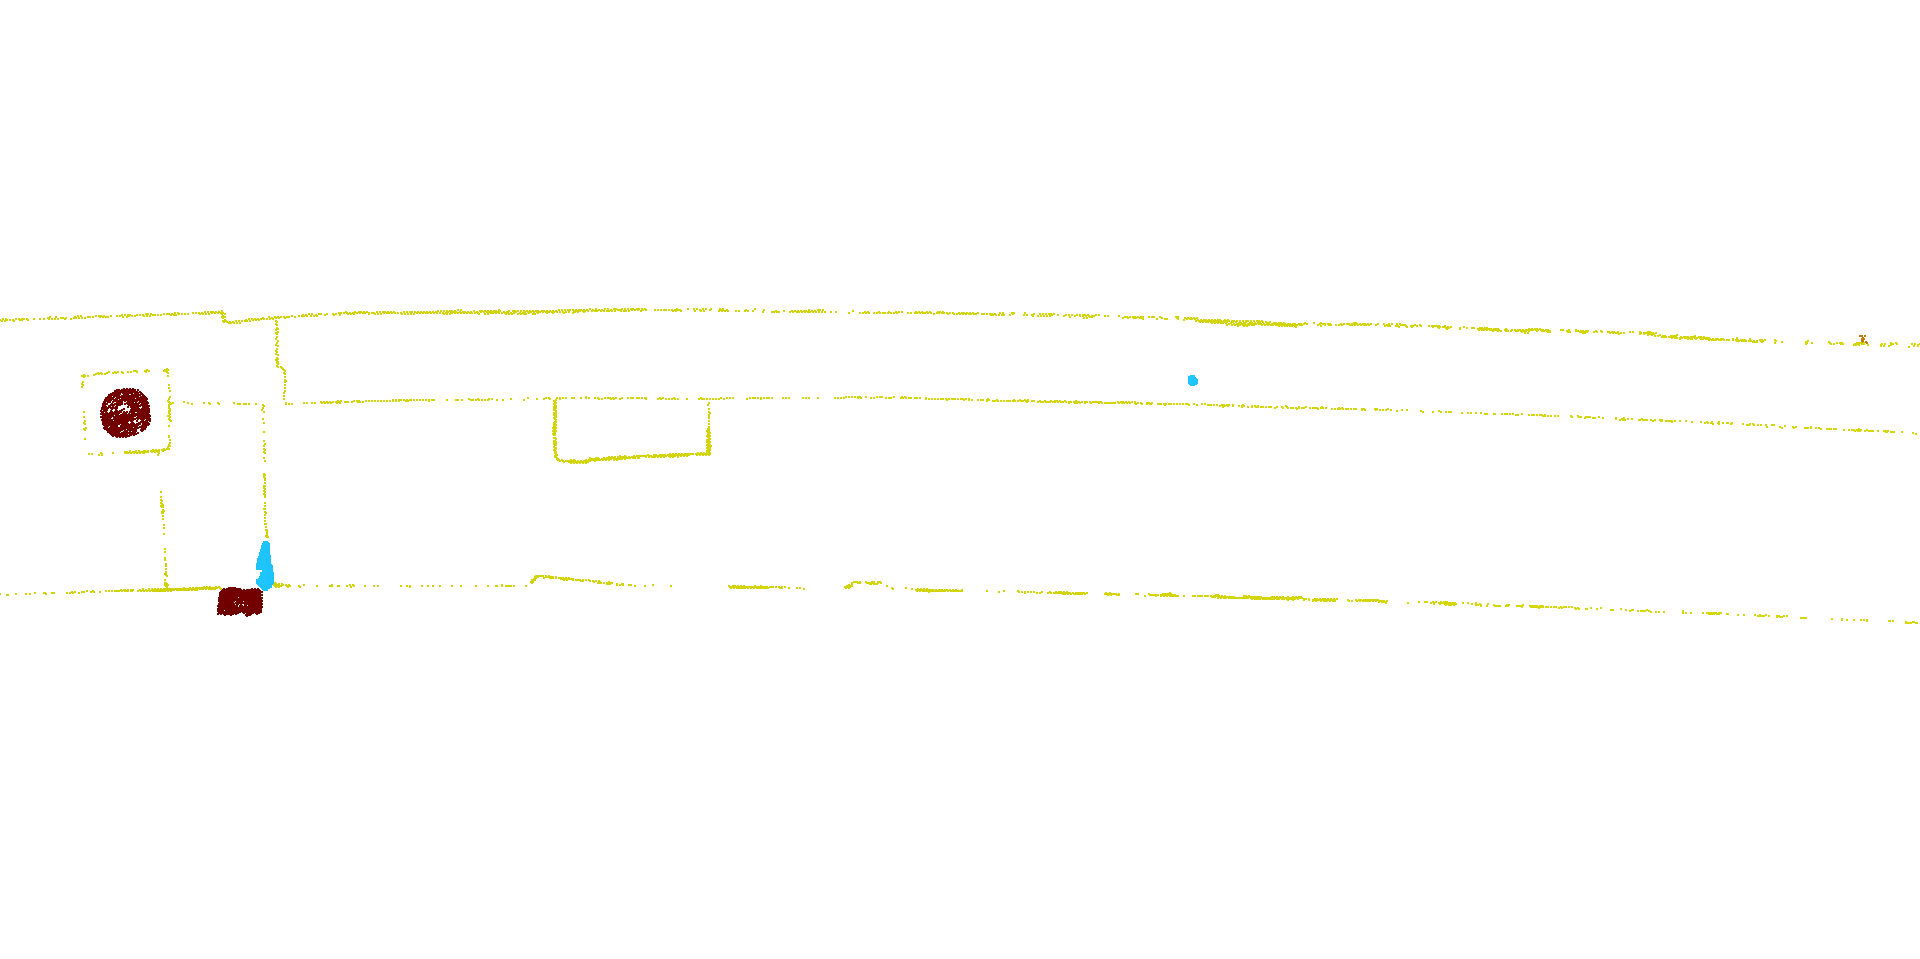
\includegraphics[width=0.96\textwidth]{graphics/eval_left_high_unique}}
    \par\smallskip
    {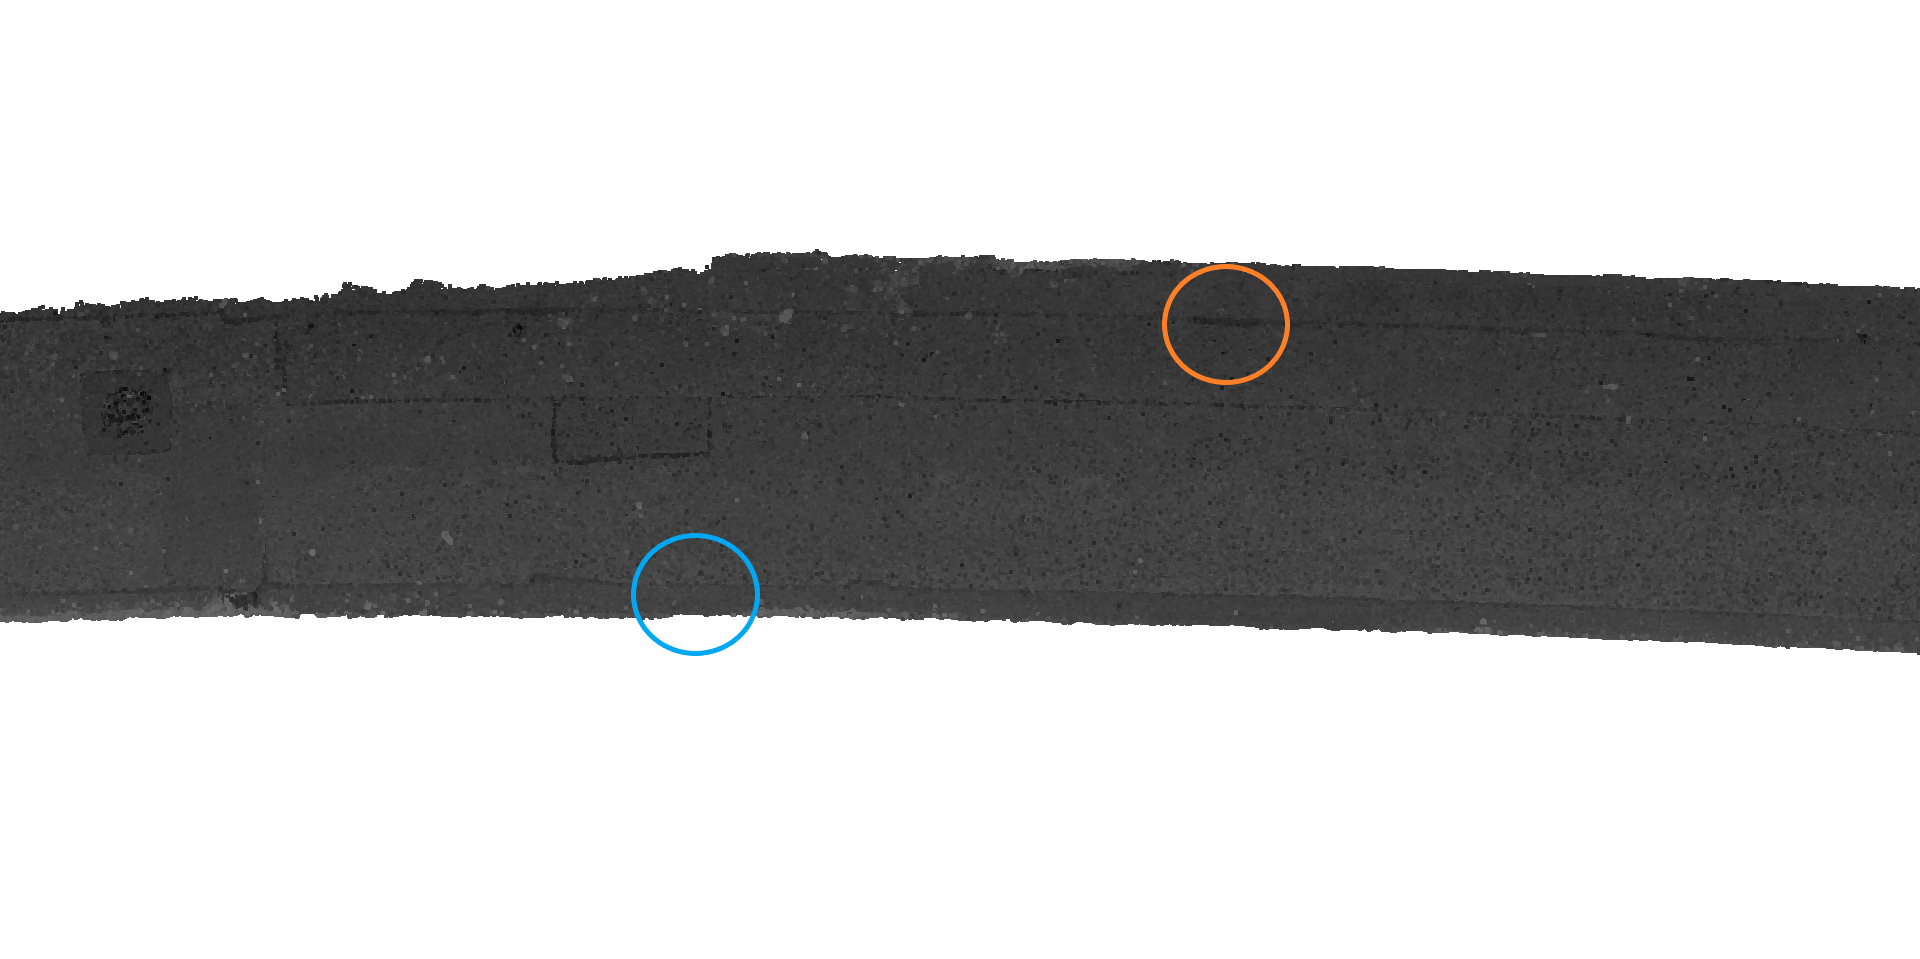
\includegraphics[width=0.96\textwidth]{graphics/eval_left_no_classes_circles}}
    \par\smallskip
    {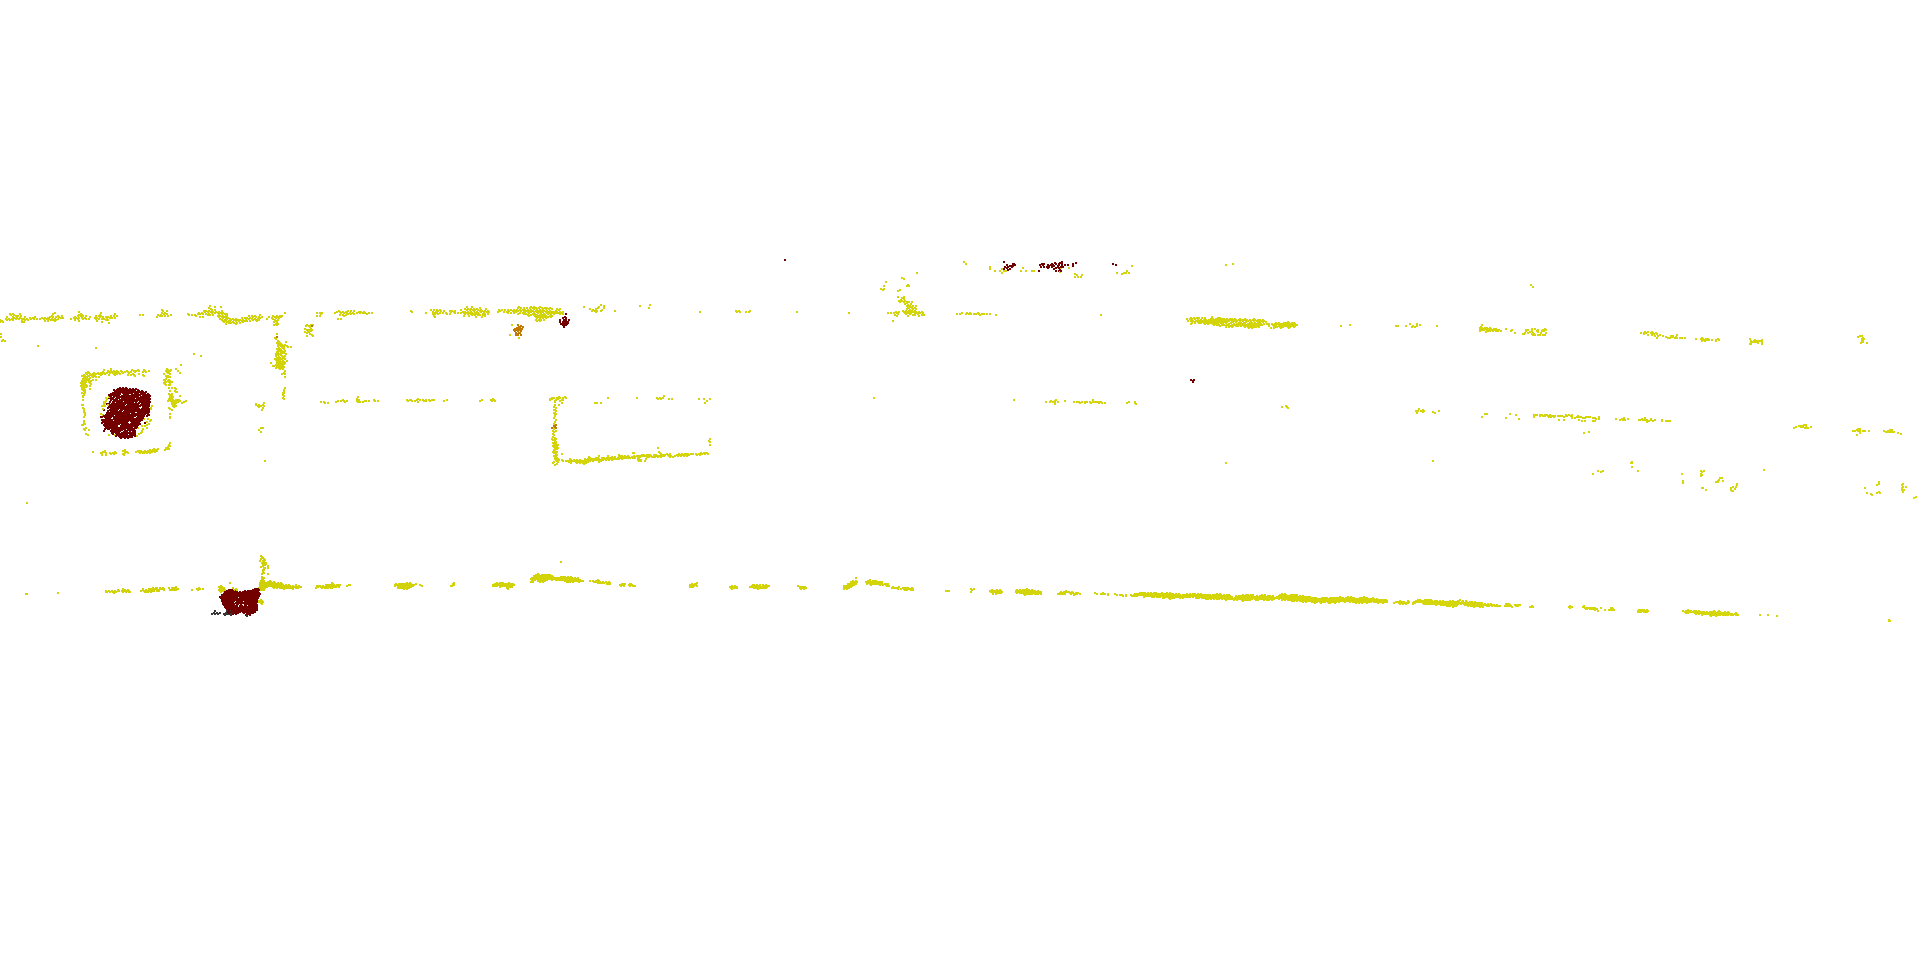
\includegraphics[width=0.96\textwidth]{graphics/eval_left_prediction}}
    \caption{Die als unique erkannten Flickstellen mit $\alpha = 3,0$ (oben), die Intensitäten der Punktwolke (mittig) und die Prediction der Flickstellen (unten).}
    \label{fig:cmp_uniqueness}
\end{figure}

\section{Ansatz Deep Learning - Ergebnisse}

Die Experimente mit \texttt{PointNet} basieren, wie in Kapitel \ref{chap:deepl} vorgestellt, auf vier wesentlichen Parametern. Für jeden im \textit{Feature-Extraction}-Ansatz genutzten Scale wird ein Experiment mit \texttt{PointNet} und entsprechendem \textit{Query Radius} durchgeführt. Der Parameter \textit{Neighborhood Size} wird dabei angenähert an die durchschnittliche Nachbarzahl des jeweiligen Scales, die sich aus Tabelle \ref{table:neighbor_counts} ergibt, und ist in Tabelle \ref{table:pointnet_params} pro Scale aufgeführt. Die Anzahl der genutzten Epochen pro Versuch liegt bei 5. Durchläufe mit mehr Epochen haben gezeigt, dass bereits frühzeitig keine Verbesserung der für das Fehlermaß genutzten Metriken mehr erfolgt, sondern diese alternieren. Der für die Experimente genutzte Wert des \textit{Length Dividers} hängt grundsätzlich vom \textit{Query Radius} ab, da bei kleinerem Scale mehr \textit{Samples} aus der Punktwolke gezogen werden müssen, um auch Punkte kleinerer Objekte mit höherer Wahrscheinlichkeit zu betrachten. Damit für diesen Vergleich nicht zu viele Parameterkombinationen zu testen sind und, da der genaue Einfluss des Parameters auf die Menge der gezogenen \textit{Samples} unklar bleibt, wird der Wert auf 500 gesetzt, was nahe der Standardbelegung liegt. 

\begin{table}
\centering
\begin{tabular}{c|c|c|c|c|c}
\textit{Query Radius} & 3$cm$ & 6$cm$ & 9$cm$ & 12$cm$ & 15$cm$ \\
\hline
\textit{Neighborhood Size} & 10 & 40 & 100 & 190 & 290 \\
\end{tabular}
\caption{Die genutzten Werte für die Neighborhood Size pro Query Radius.}
\label{table:pointnet_params}
\end{table}

Während das Training mit \textit{Samples} arbeitet, funktioniert die \textit{Prediction} in \texttt{PCNN} mit einem \textit{Full Covering Dataset}. Das bedeutet, dass alle Punkte garantiert in mindestens einer betrachteten Nachbarschaft vorkommen und ihnen somit eine Klasse zugewiesen wird. Gerade für die zum Teil feinen Objekte, die in dieser Arbeit betrachtet werden, ist die Verwendung aller Punkte bedeutsam, um nicht etwa ein kleines Schlagloch auszulassen und nicht zu klassifizieren. Die Erstellung dieses Datensatzes macht den größeren Teil der \textit{Prediction}-Laufzeit aus im Vergleich zu den schnellen Berechnungen des trainierten neuronalen Netzes. Je nach \textit{Query Radius} und \textit{Length Divider} variiert die Laufzeit für die Testpunktwolke von 50$s$ bis hin zu 10$min$. Obwohl erstere Zeit deutlich geringer ist als die vom \textit{Feature-Extraction}-Ansatz, lässt sich festhalten, dass die Laufzeiten in derselben Größenordnung liegen. Das Training von \texttt{PointNet} benötigt auch bei wenigen Epochen deutlich länger als das der \textit{Random Forests}, da hier auch die komplexeren Berechnungen dahinterstehen. Die Trainingszeit ist für diesen Anwendungsfall aber zu vernachlässigen, da es ohnehin nur einmalig stattfindet. \\

In Abbildung \ref{fig:cmp_pointnet_right} sind Ausschnitte zweier \textit{Predictions} von \texttt{PointNet} zu sehen und im Vergleich dazu die des \textit{Feature-Extraction}-Ansatzes. Die Werte für den \textit{Query Radius} sind dabei der minimale sowie maximale genutzte Scale, 3$cm$ und 15$cm$, um die Unterschiede zwischen diesen ebenfalls herauszuarbeiten. Ein anderer Abschnitt der Testpunktwolke mit denselben \textit{Predictions} ist in Abbildung \ref{fig:cmp_pointnet_left} zu finden. \\
Für beide Scales lässt sich beobachten, dass die tatsächliche Fahrbahnmarkierung in ähnlichem Maße wie beim \textit{Feature-Extraction}-Ansatz klassifiziert wird. Deren hintere dunklere Stellen bereiten somit beiden Ansätzen Probleme. Bei den \texttt{PointNet}-Ergebnissen fällt jedoch auf, dass am unteren Rand der Punktwolke auch komplette Streifen fälschlich als Fahrbahnmarkierung klassifiziert werden. Diese Stellen besitzen in der Tat hohe Intensitäten, die \texttt{PointNet} nicht richtig unterscheiden lassen. Im kleinen Scale werden die Ölflecken als Schlaglöcher markiert, was vermutlich an den geringen Intensitäten beider Klassen liegt, wobei die Ölflecken keine derart gekrümmten Oberflächen besitzen. Im 15$cm$-Scale werden die Ölflecken aber größtenteils korrekt klassifiziert, wobei dort der kleine Gully am rechten Rand ebenfalls zu den Ölflecken gezählt wird. Für den gegenüberliegenden, gleichartig gebauten Gully gilt dies jedoch nicht, womöglich wegen einer leicht geringeren Intensität. Ansonsten ist die Klassifizierung der Gullys erwartbar: Was im kleineren Scale in der planaren Mitte noch fehlt, kann der größere Scale fast vollständig auffüllen. Auch der runde Gully in den zweiten Bildern wird im größeren Scale sehr viel präziser und vollständiger klassifiziert. \\
Die tatsächlich vorhandenen Schlaglöcher werden bereits im kleinen Scale und noch besser im größeren Scale erkannt - außer das längliche Schlagloch, das in keinem Experiment als solches klassifiziert wurde und in den Trainingsdaten nicht repräsentiert ist. Daneben gibt es jedoch auch viel Rauschen in dieser Klasse. Während im kleinen Scale, wie erwähnt, die Ölflecken als Schlaglöcher gesehen werden, gilt dies im größeren Scale für Teile der Flickstellen. Diese ähneln sich in der Form grundsäzlich nicht, aber die Intensität kann ähnlich und eine Flickstelle auch leicht erhöht sein, wenn die Fugendichtmasse etwas austritt. Dies waren womöglich die Gründe für die Entscheidung. Die größte Schwäche der \textit{Predictions} von \texttt{PointNet} zeigt sich in der Klasse der Flickstellen. Im kleinen Scale werden dabei, auch bedingt durch das sehr große Rauschen, noch einige Punkte korrekt klassifiziert. Im großen Scale wird nahezu kein Punkt mehr als Flickstelle markiert, wobei ohnehin die Vermutung besteht, dass Flickstellen sich eher im kleinen Scale abheben. 
Schließlich sind die Metriken der beiden \texttt{PointNet}-Ergebnisse in den Tabellen \ref{table:pointnet_3_metrics} und \ref{table:pointnet_15_metrics} dargestellt, in denen sich die angesprochenen Auffälligkeiten widerspiegeln. Zukünftig wäre es interessant zu testen, ob die Ergebnisse durch weitere Trainingsdaten oder auch nur durch verlängertes Training wesentlich gebessert werden können.

\begin{figure}
    {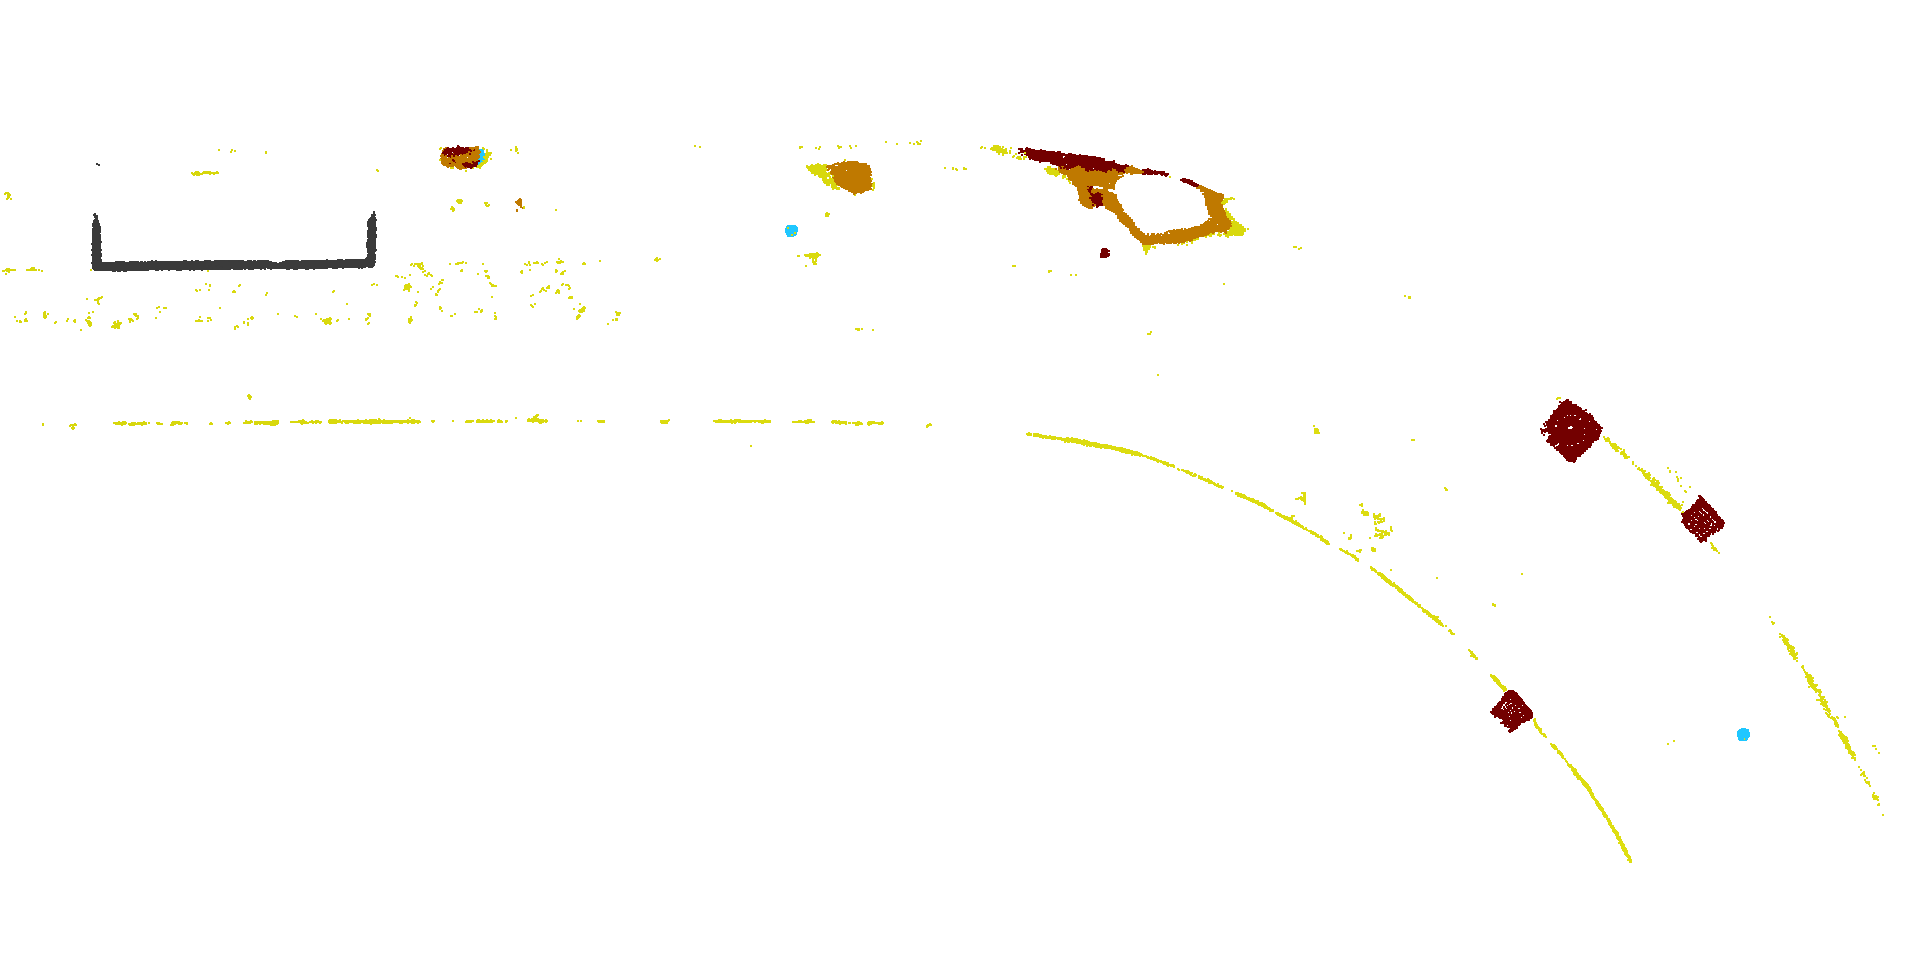
\includegraphics[width=0.96\textwidth]{graphics/eval_right_prediction}}
    \par\smallskip
    {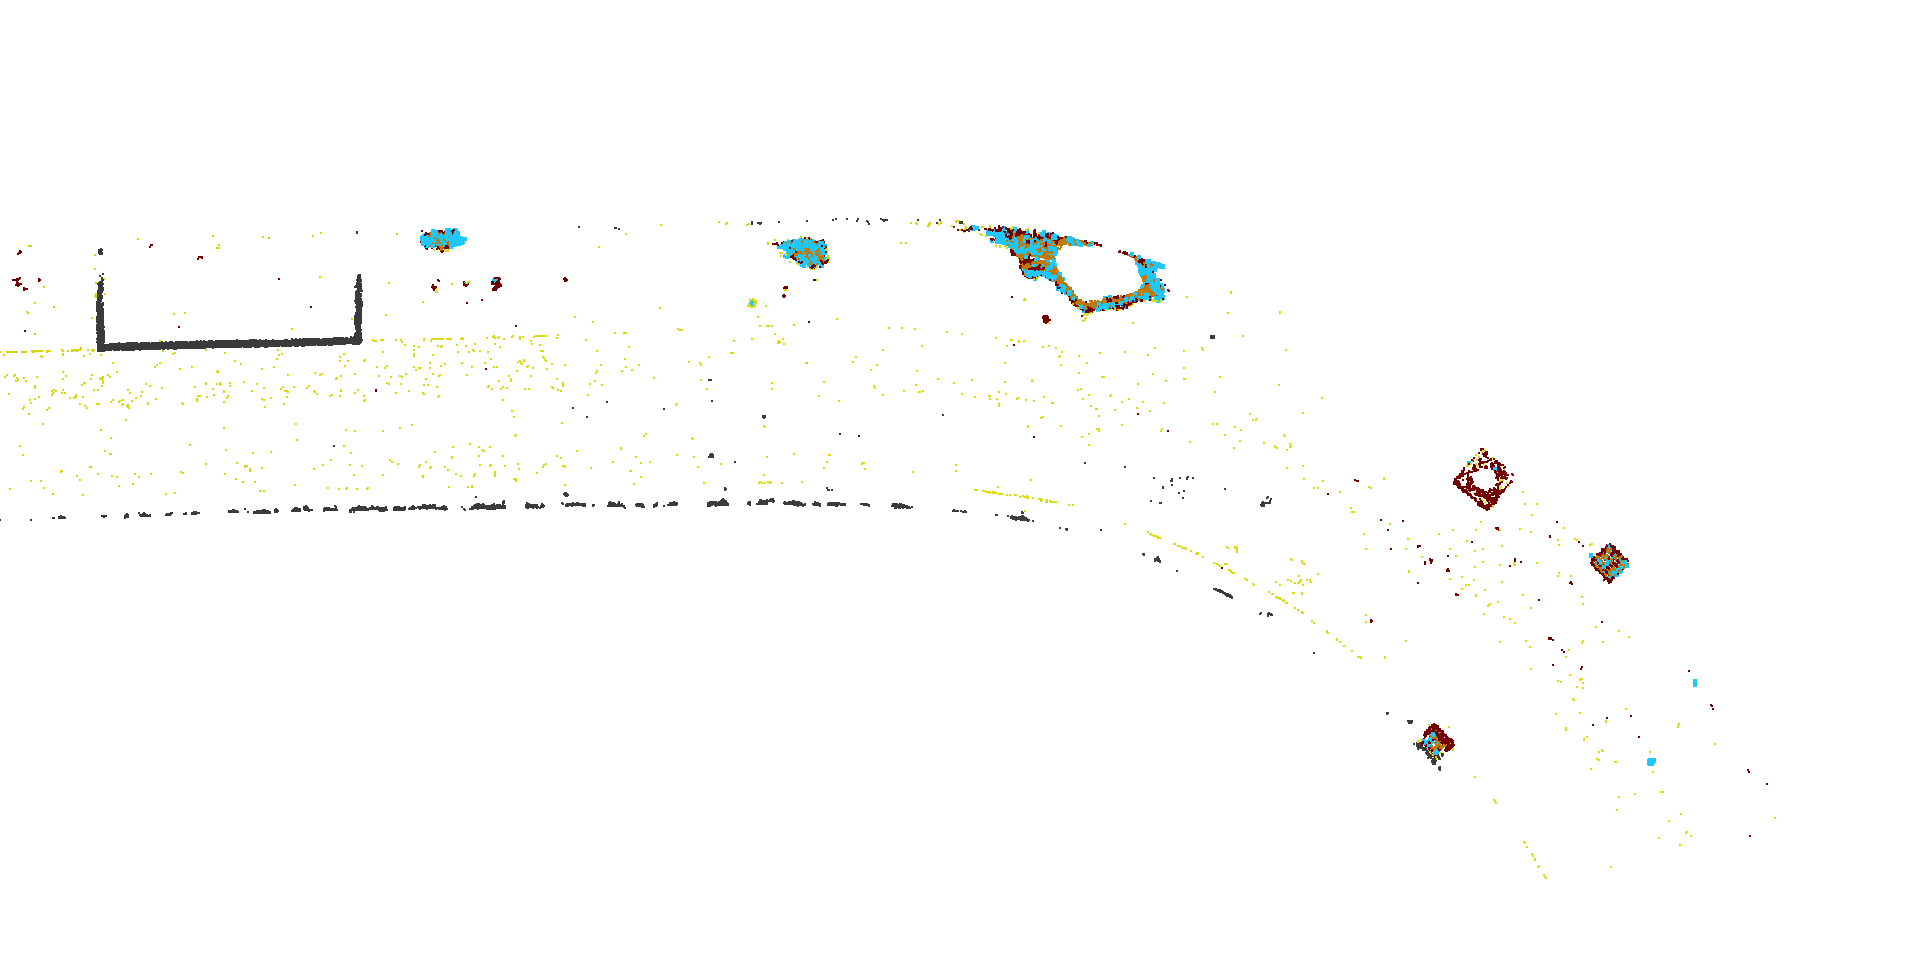
\includegraphics[width=0.96\textwidth]{graphics/eval_pointnet_3_right}}
    \par\smallskip
    {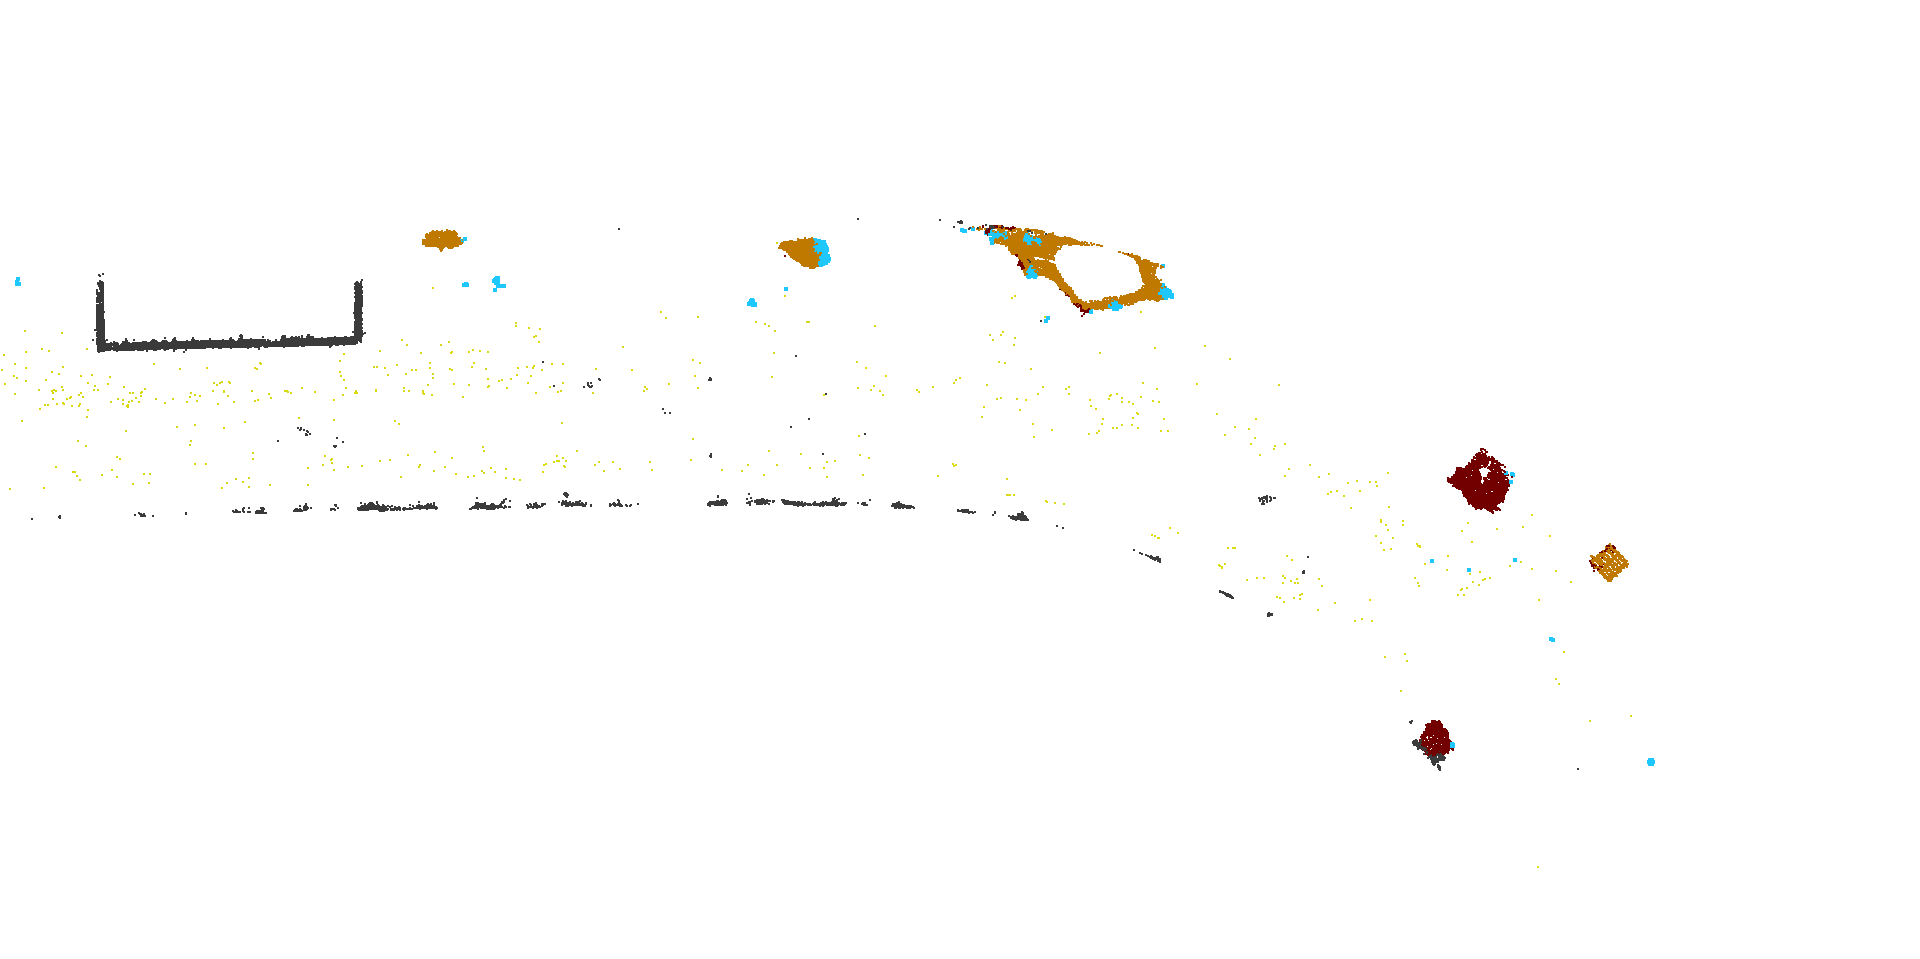
\includegraphics[width=0.96\textwidth]{graphics/eval_pointnet_15_right}}
    \caption{Die Prediction des Feature-Extraction-Ansatzes (oben), von \texttt{PointNet} mit Scale von 3cm (mittig) und von \texttt{PointNet} mit Scale von 15cm (unten).}
    \label{fig:cmp_pointnet_right}
\end{figure}

\begin{figure}
    {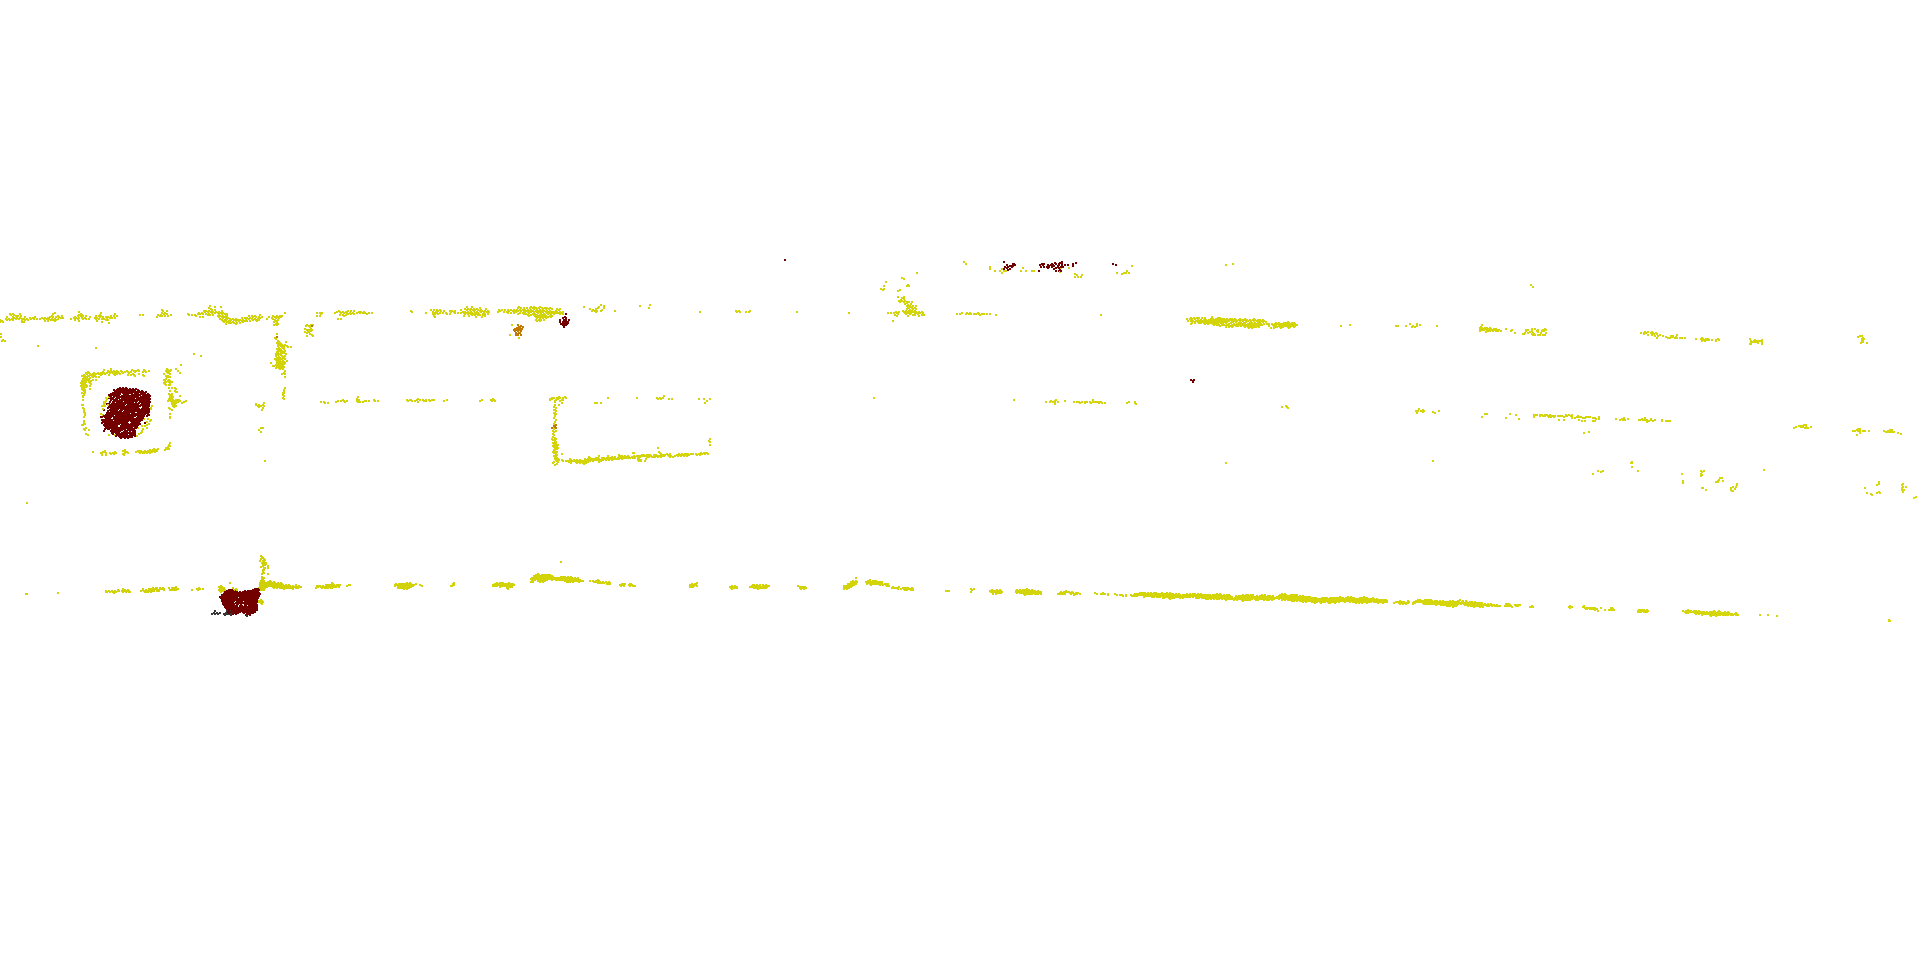
\includegraphics[width=0.96\textwidth]{graphics/eval_left_prediction}}
    \par\smallskip
    {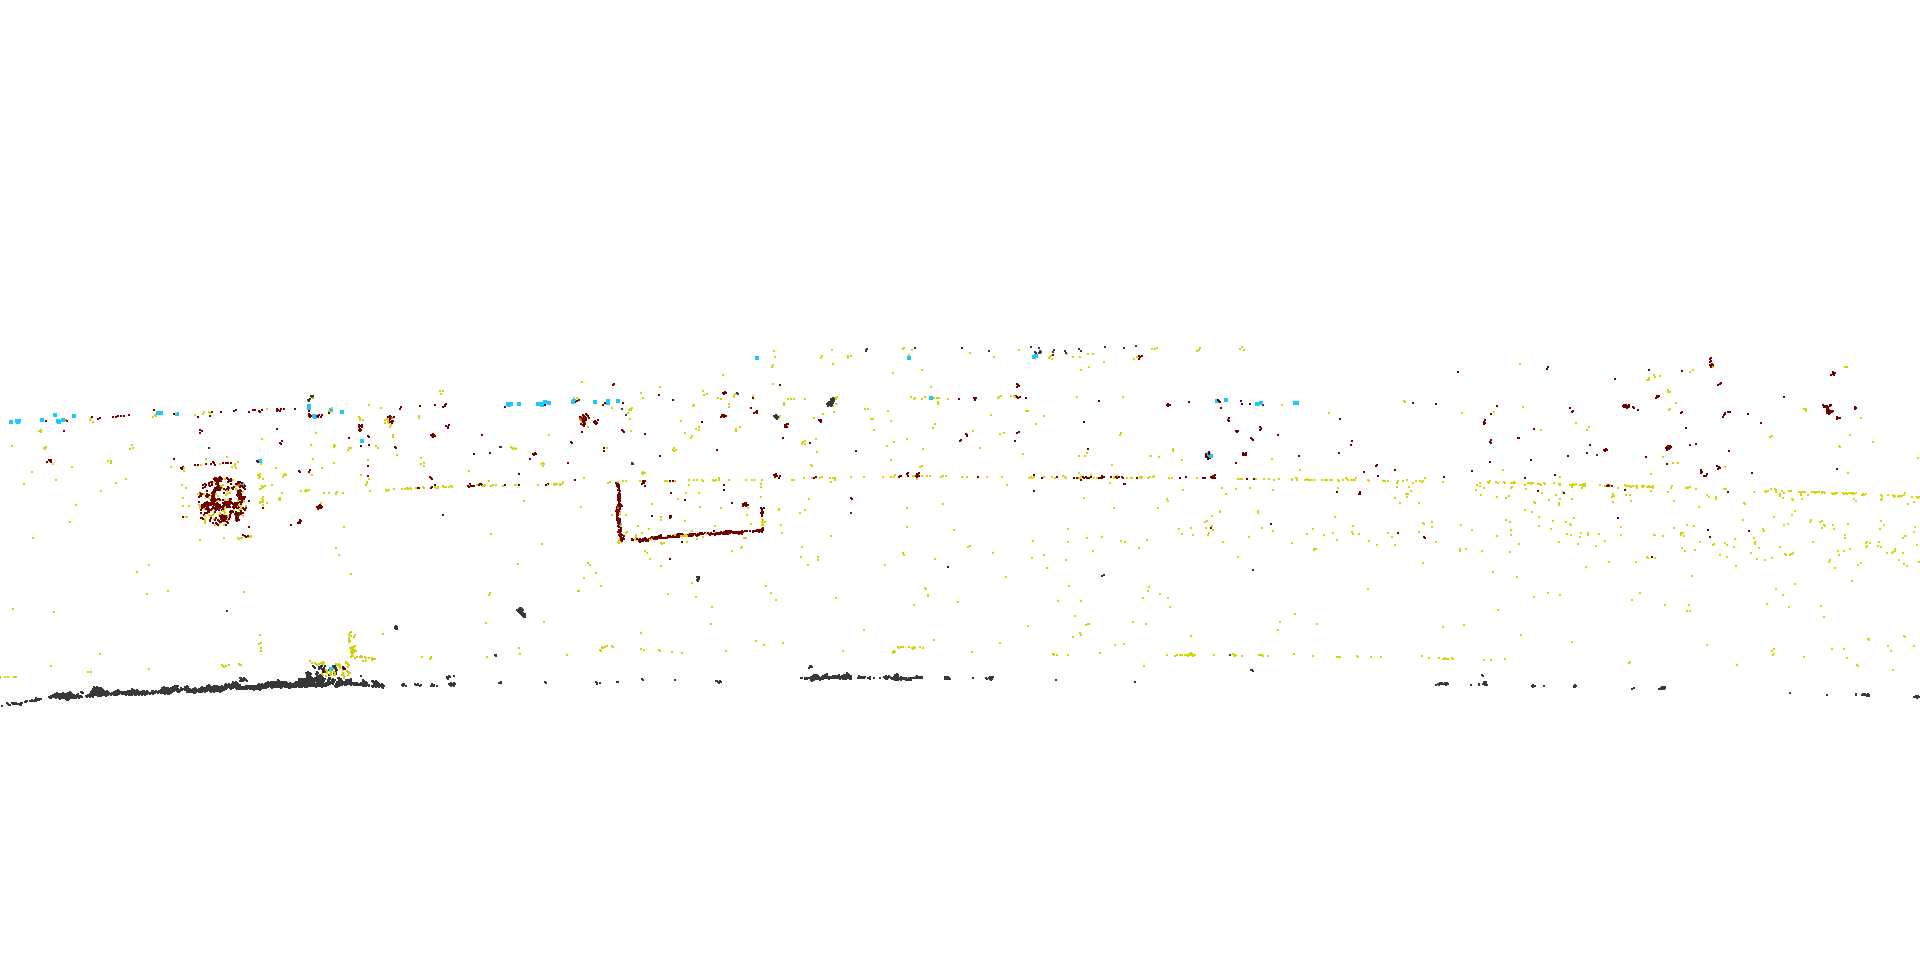
\includegraphics[width=0.96\textwidth]{graphics/eval_poinnet_3_left}}
    \par\smallskip
    {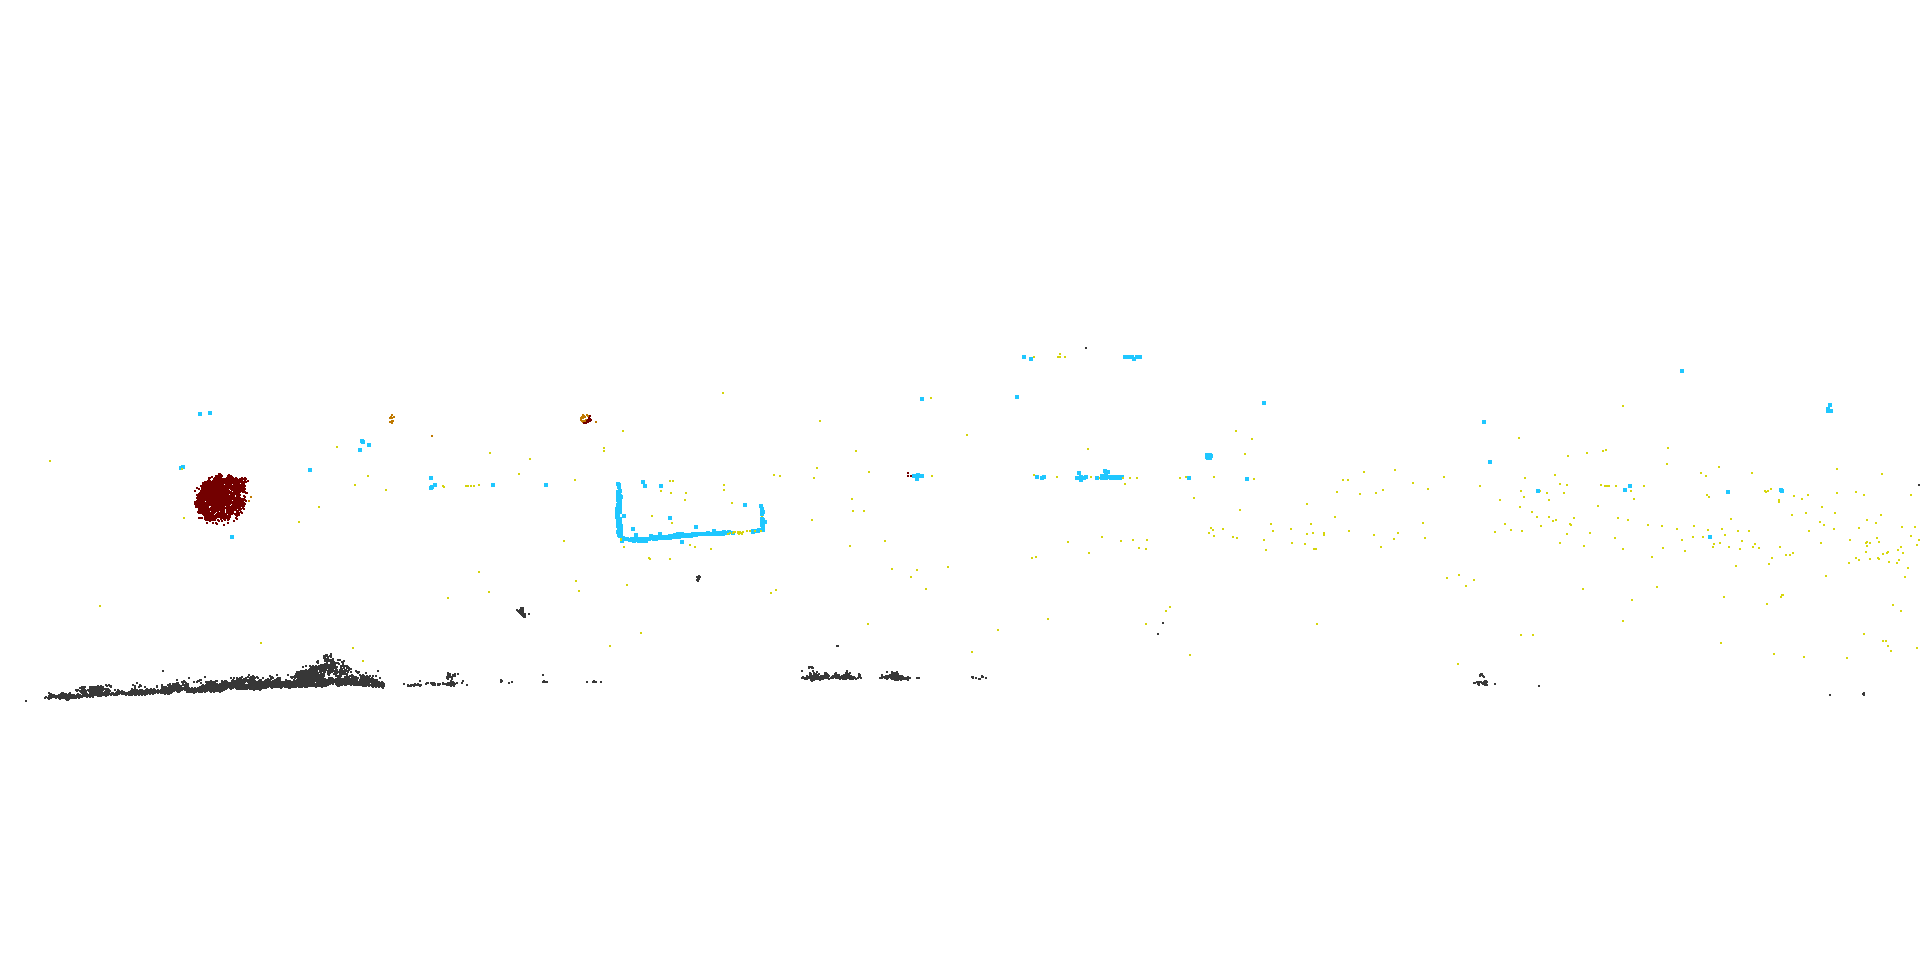
\includegraphics[width=0.96\textwidth]{graphics/eval_poinnet_15_left}}
    \caption{Die Prediction des Feature-Extraction-Ansatzes (oben), von \texttt{PointNet} mit Scale von 3cm (mittig) und von \texttt{PointNet} mit Scale von 15cm (unten).}
    \label{fig:cmp_pointnet_left}
\end{figure}


\begin{table}
\centering
\begin{tabular}{c|c|c|c|c|c|c}
 & \textit{U} & \textit{S} & \textit{F} & \textit{G} & \textit{Ö} & \textit{M} \\
\hline
Precision & 0,984 & 0,024 & 0,322 & 0,366 & 0,841 & 0,254 \\
Recall    & 0,992 & 0,053 & 0,063 & 0,303 & 0,377 & 0,658 \\
F1        & 0,988 & 0,033 & 0,105 & 0,332 & 0,521 & 0,367 \\
\end{tabular}
\caption{Die Metriken der einzelnen Klassen für das \texttt{PointNet}-Experiment im Scale von 3$cm$.}
\label{table:pointnet_3_metrics}
\end{table}

\begin{table}
\centering
\begin{tabular}{c|c|c|c|c|c|c}
 & \textit{U} & \textit{S} & \textit{F} & \textit{G} & \textit{Ö} & \textit{M} \\
\hline
Precision & 0,984 & 0,110 & 0,124 & 0,769 & 0,853 & 0,268 \\
Recall    & 0,994 & 0,135 & 0,006 & 0,573 & 0,745 & 0,686 \\
F1        & 0,989 & 0,121 & 0,011 & 0,656 & 0,796 & 0,386 \\
\end{tabular}
\caption{Die Metriken der einzelnen Klassen für das \texttt{PointNet}-Experiment im Scale von 15$cm$.}
\label{table:pointnet_15_metrics}
\end{table}

\section{Postprocessing}
\label{section:postproc}

Die Auswirkungen des \textit{Postprocessings} werden im Folgenden für beide Ansätze dargestellt. Da die Metriken pro Klasse nahezu keine Änderung erfahren, soll die Auswertung auf Bildbasis erfolgen.
Für die erste Richtung der Nachverarbeitung, der Entfernung von (bezüglich ihrer Klasse) Außenseitern, sind in Abbildung \ref{fig:cmp_postproc} erneut die \textit{Prediction} des Basisexperiments sowie das Ergebnis des \textit{Postprocessings} zu sehen. Wie grundsätzlich zu erkennen ist, betrifft dieser Schritt größtenteils die als Flickstelle klassifizierten Punkte, da gerade diese oft unbeständig gefunden werden. Insbesondere im Umkreis der Fahrbahnmarkierung wird deutlich, dass ein großer Teil der fälschlich als Flickstelle klassifizierten Punkte entfernt bzw. wieder der gewöhnlichen Straßenklasse zugewiesen wird. Größere \textit{Cluster} darin bleiben hingegen, wie erwartet, bestehen. Auch kleine Gruppen von Flicktellen um Schlaglöcher herum werden richtig korrigiert. \\
Auf der anderen Seite ist bei genauem Blick erkennbar, dass zum Teil auch korrekte Klassifizierungen von Flickstellen zurückgenommen werden. Dies passiert bei lückenhaften Stellen oder dort, wo nur sehr feine Linien als Flickstelle klassifiziert wurden. Die rechteckige Form bleibt im Gesamten dennoch zu erkennen. Bei der Entscheidung für oder gegen diesen Schritt muss daher eine Abwägung getroffen werden zwischen der \textit{Precision} und dem \textit{Recall} der Flickstellen, wobei durch das \textit{Postprocessing} erstere steigt und letzterer sinkt. Die Laufzeit dieses Schritts ist mit 15$s$ verhältnismäßig gering. \\

\begin{figure}
    {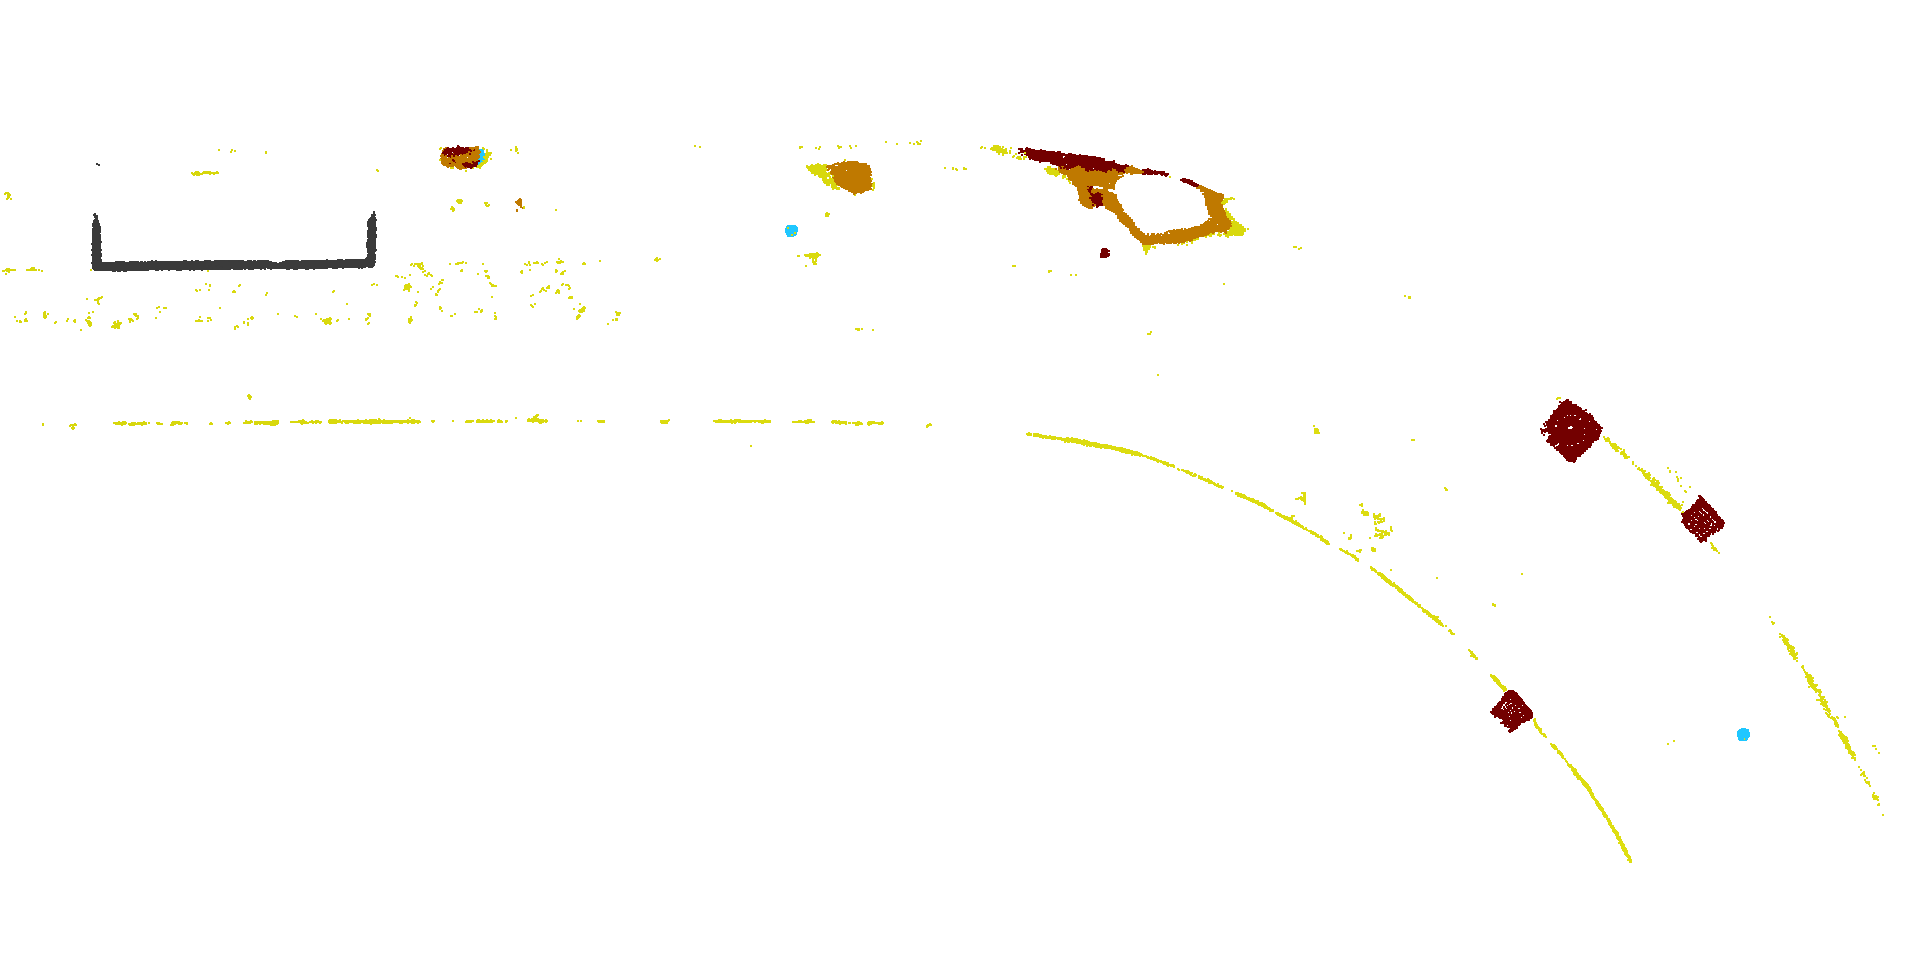
\includegraphics[width=0.96\textwidth]{graphics/eval_right_prediction}}
    \par\smallskip
    {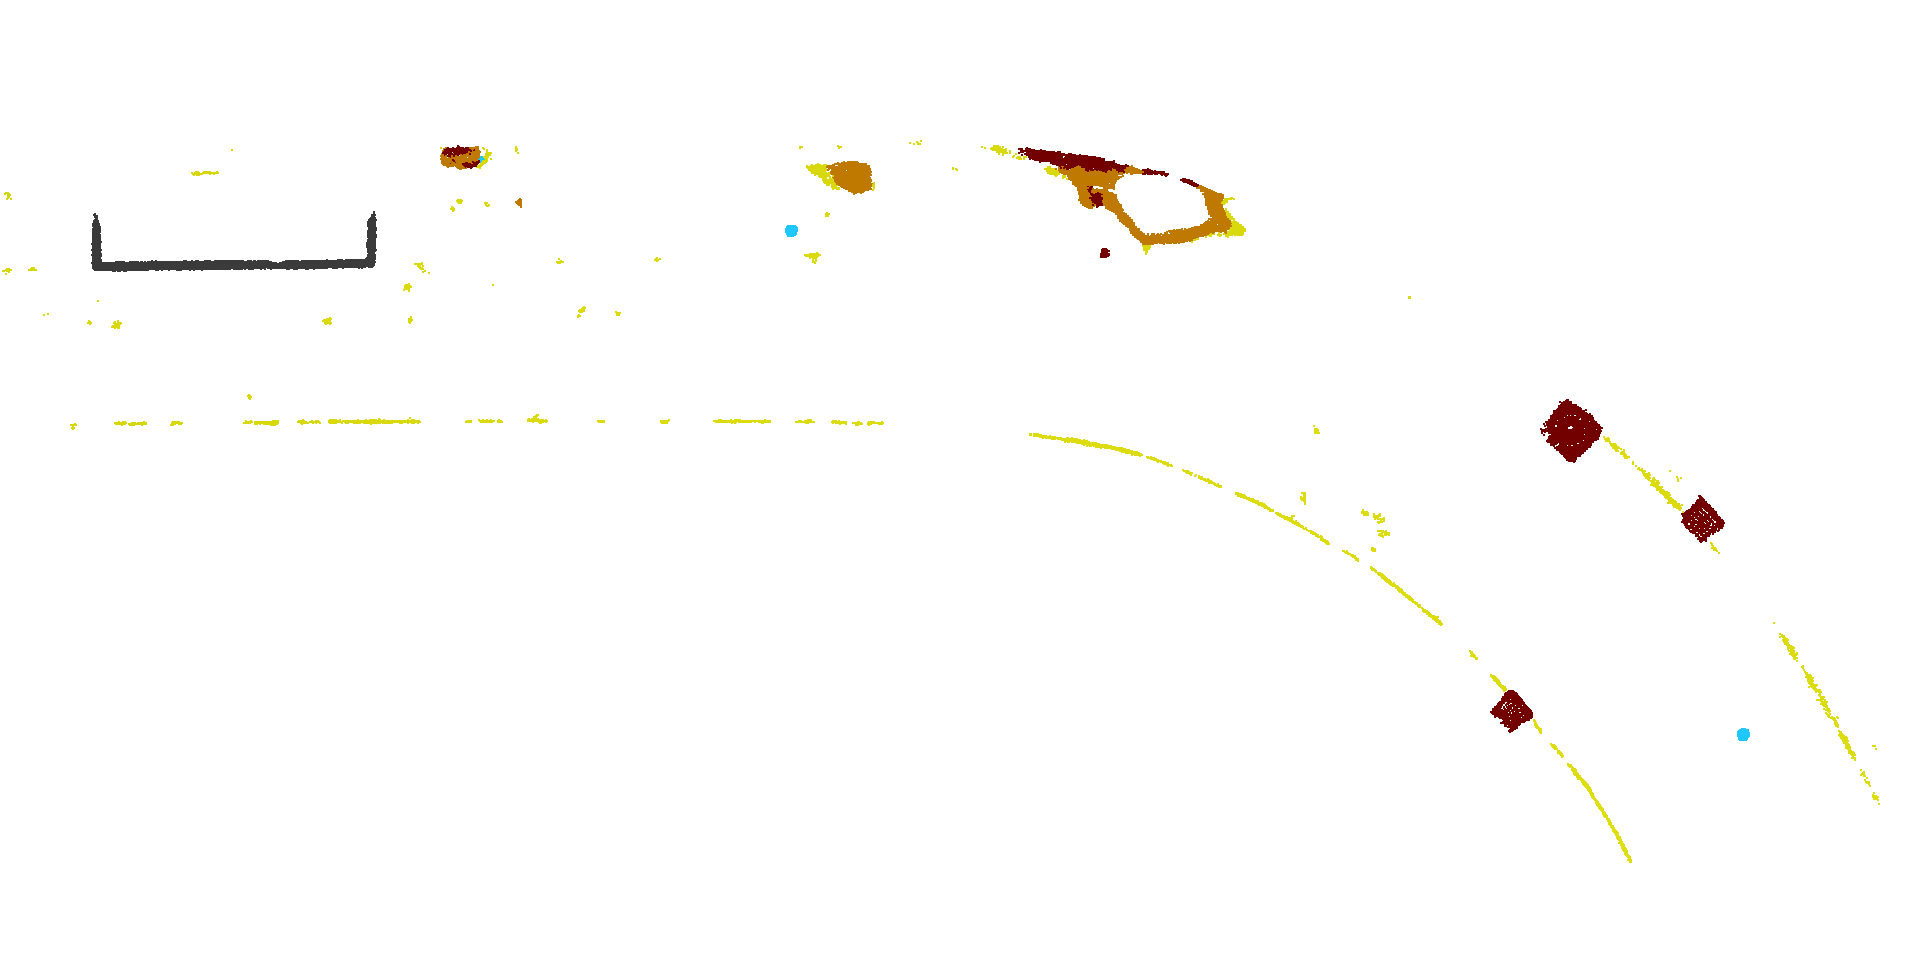
\includegraphics[width=0.96\textwidth]{graphics/eval_right_postproc}}
    \caption{Die Prediction vor (oben) und nach (unten) dem Postprocessing.}
    \label{fig:cmp_postproc}
\end{figure}

Durch die zweite Iteration des \textit{Postprocessings}, dem ``Auffüllen'' von Klassen anhand von Außenseiter-Straßenpunkten, wird die Klasse keines Punktes geändert. Tatsächlich liegen in der \textit{Prediction} keine Bodenpunkte etwa inmitten von Schlaglöchern. Lediglich die mittleren Stellen von Gullys kämen in Frage, für die ein größerer Scale nötig wäre. Die Anpassung der \textit{Postprocessing}-Parameter für die Korrektur dieser Punkte verursacht jedoch an zahlreichen anderen Stellen ungewünschte Effekte, indem \textit{Cluster} von Fehlklassifzierungen noch größer werden. Diese Iteration bringt also keine Verbesserungen und ihre Ausführung dauert - wegen der großen Zahl an Straßenpunkten - auch deutlich länger als die der ersten, etwa 90$s$. Aus diesen Gründen wird die zweite Iteration nicht mehr ausgeführt. \\\\
An dieser Stelle soll auch die Auswirkung der ersten Iteration auf die \textit{Prediction} von \texttt{PointNet} erwähnt werden, wobei diejenige mit Scale von 15$cm$ betrachtet wurde. Dabei ist vor allem zu erkennen, wie die vielen einzelnen Punkte, die als Flickstelle klassifiziert wurden, zurück als Straßenpunkte gesetzt werden. Anschließend besitzt kaum ein Punkt überhaupt mehr die Klasse Flickstelle. Ein paar andere Außenseiterpunkte der Schlaglöcher und Fahrbahnmarkierungen werden ebenfalls entfernt, was die $F1-Scores$ um jeweils einen Prozentpunkt steigert. Allerdings wird hieran auch deutlich, dass das \textit{Postprocessing} in dieser Form nicht für \textit{Predictions} gedacht ist, die besonders viel Rauschen beinhalten. Die Idee und die verwendeten Parameter wurden motiviert durch Ergebnisse des \textit{Feature-Extraction}-Ansatzes und müssten bei Bedarf angepasst werden.

\section{Zusammenfassung} 

Insgesamt lässt sich festhalten: Der \textit{Feature-Extraction}-Ansatz funktioniert bei keiner Klasse besonders schlecht und verursacht verhältnismäßig wenig Rauschen. \texttt{PointNet} kann im größeren Scale Gullys gut erkennen und findet teils Schlaglöcher, die der eigene Ansatz nicht entdeckt oder als Gullys klassifiziert hat. Probleme hat \texttt{PointNet} vor allem bei Flickstellen und verursacht sehr großes Rauschen in den Klassifizierungen. Dennoch ist die Leistung von \texttt{PointNet} hoch einzustufen, da dieses jeweils nur einen Scale zur Verfügung hat im Gegensatz zu den \textit{Random Forests}. Außerdem wurden sich für den \textit{Feature-Extraction}-Ansatz manuell und mit Blick auf die Daten aussagekräftige Features überlegt, wohingegen das neuronale Netz diese eigenständig extrahieren muss. \\
Aus diesem Grund wirkt ein Einsatz von \texttt{PointNet} zur Erkennung von Straßenschäden auf der Webplattform vielversprechend. Dennoch sollen zunächst weitere Konfigurationen seiner Parameter oder ein gänzlich anderer \textit{Deep-Learning}-Ansatz getestet und erst einmal der \textit{Feature-Extraction}-Ansatz auf Basis der \textit{Random Forests} genutzt werden. Langfristig bietet sich der Einsatz eines \textit{Deep-Learning}-Ansatzes aber an, da die Plattform bereits über einen Optimierungsmechanismus solcher Modelle verfügt und auf diese Weise automatisch deren Ergebnisse weiter verbessern könnte.